% --------------------------
% ---- DECLARE PACKAGES ----
% --------------------------
\documentclass[a4paper, oneside, openright]{book}

% PDF/A-2b
\usepackage[a-2b]{pdfx}

\usepackage[T1]{fontenc} % Font encoding, T1 = it
\usepackage{lmodern}
\usepackage{multicol} % Per il frontespizio
\usepackage[utf8]{inputenc} % Input encoding
\usepackage[english,italian]{babel} % Lingua principale italiana, con parti in inglese
\usepackage{minted} % Per i blocchi di codice
\usepackage{csquotes} % Dipendenza di babel e biblatex
\usepackage{graphicx} % Immagini esterne

\usepackage{setspace}
\onehalfspacing % interlinea 1.5

\usepackage[parfill]{parskip} % Disabilita l'indentazione dopo essere andati a capo
\usepackage{titlesec}
\usepackage{float}
\usepackage{booktabs}
\usepackage{longtable}
\usepackage{tabularx}
\usepackage{multirow}
\usepackage{enumitem}
\usepackage{amsmath}
\usepackage{amssymb}

% Colonne di tabella a bandiera
\newcolumntype{L}{>{\raggedright\arraybackslash}X}
\newcolumntype{P}[1]{>{\raggedright\arraybackslash}p{#1}}
\newcolumntype{B}[1]{>{\raggedright\arraybackslash\bfseries}p{#1}}

% Percorso immagini
\graphicspath{{Immagini/}{Immagini/Sessioni/}{Immagini/Screenshot/}}

% Diagrammi TikZ
\usepackage{tikz}
\usepackage{pgfplots}
\pgfplotsset{compat=1.18}
\usetikzlibrary{shapes.geometric, shapes.multipart, arrows, arrows.meta,
                positioning, fit, backgrounds, calc, chains, automata,
                decorations.pathreplacing}
\tikzstyle{startstop} = [rectangle, rounded corners, minimum width=3cm, minimum height=1cm,text centered, draw=black, fill=red!30]
\tikzstyle{io} = [trapezium, trapezium left angle=70, trapezium right angle=110, minimum width=3cm, minimum height=1cm, text centered, draw=black, fill=blue!30]
\tikzstyle{process} = [rectangle, minimum width=3cm, minimum height=1cm, text centered, draw=black, fill=orange!30]
\tikzstyle{decision} = [diamond, minimum width=3cm, minimum height=1cm, text centered, draw=black, fill=green!30]
\tikzstyle{arrow} = [thick,->,>=stealth]

% Stili per i diagrammi
\tikzset{
  layer/.style   = {rectangle, rounded corners=3pt, draw=black!70, thick,
                    align=center, inner sep=6pt, minimum height=1cm},
  comp/.style    = {rectangle, rounded corners=2pt, draw=black!60,
                    fill=white, align=center, font=\footnotesize,
                    inner sep=4pt, minimum height=0.8cm},
  extern/.style  = {rectangle, dashed, draw=black!60, align=center,
                    font=\footnotesize, inner sep=4pt},
  ucase/.style   = {ellipse, draw=black!70, align=center,
                    font=\footnotesize, inner sep=2pt, minimum width=2.6cm},
  flow/.style    = {-{Latex[length=2mm]}, thick},
  flowdash/.style= {-{Latex[length=2mm]}, thick, dashed},
  % Stili per i diagrammi
  tile/.style    = {rectangle, draw=black!55, fill=black!2, thin},
  cellgrid/.style= {draw=black!35, thin, dash pattern=on 1.2pt off 1.2pt},
  pin/.style     = {circle, fill=black!75, draw=none, inner sep=0pt,
                    minimum size=3pt},
  bubble/.style  = {circle, draw=black!65, fill=black!12, thick,
                    inner sep=0pt, font=\scriptsize},
  tick/.style    = {black!70, thin},
  band/.style    = {rectangle, draw=black!55, fill=black!6, rounded corners=1pt}
}

% Captions
\usepackage[font=scriptsize, skip=5pt, justification=centering]{caption}

\usepackage[backend=biber, style=numeric, backref=true, defernumbers=true]{biblatex}

% Per sitografia
\setcounter{biburlnumpenalty}{7000}
\setcounter{biburlucpenalty}{7000}
\setcounter{biburllcpenalty}{7000}

\usepackage[immediate]{silence}
\WarningFilter[temp]{latex}{Command}
\usepackage{sectsty}
\DeactivateWarningFilters[temp]

% Impaginazione e margini
\usepackage[fontsize=12pt]{scrextend} % dimensione font

% footmisc
\usepackage[bottom]{footmisc}
\usepackage{hyperref}
\usepackage{subcaption}

% Sperimentali
\WarningFilter{microtype}{Unable to apply patch `footnote'}
\usepackage{microtype}

\usepackage[top=3.5cm,bottom=3.5cm,left=3.5cm,right=3.5cm]{geometry}

% Aspetto liste
\setminted{
  fontsize=\small,
  breaklines=true,
  breakanywhere=true,
  tabsize=2,
  frame=lines,
  framesep=6pt,
  xleftmargin=0pt
}
\renewcommand{\listingscaption}{Listato}
\renewcommand{\listoflistingscaption}{Elenco dei listati}

% ------------------------
% ---- DOCUMENT SETUP ----
% ------------------------
\pagestyle{plain}
\raggedbottom

\titleformat{\chapter}[display]
{\normalfont\huge\bfseries}{\chaptertitlename\ \thechapter}{10pt}{\LARGE}
\titlespacing*{\chapter}{0pt}{0pt}{20pt}
\chaptertitlefont{\fontsize{22pt}{30pt}\selectfont}

% Titoli
\sectionfont{\raggedright}
\subsectionfont{\raggedright}
\subsubsectionfont{\raggedright}

\hypersetup{
    colorlinks,
    citecolor=black,
    filecolor=black,
    linkcolor=black,
    urlcolor=black
}

\renewcommand{\footnotesize}{\fontsize{11pt}{13pt}\selectfont} % Imposta la dimensione del testo delle footnotes
\setlength{\footnotesep}{0.5cm} % Imposta lo spazio fra le singole footnotes
\setlength{\skip\footins}{1.5cm} % Imposta lo spazio fra il corpo e le footnotes

\DeclareUnicodeCharacter{02BC}{}

% ------------------------
% ---- DOCUMENT START ----
% ------------------------
\addbibresource{bibliography.bib} % Bibliografia
\begin{document} % Inizio documento
\hypersetup{pageanchor=false}
\frontmatter
\begin{titlepage}
\begin{figure}[!htb]
    \centering
    
\includegraphics[width=5cm]{Immagini/uninsubria-logo}
\end{figure}

\begin{center}
    \Large{\textbf{UNIVERSITÀ DEGLI STUDI DELL'INSUBRIA}}
    \vspace{3mm}
    \\ \normalsize{DIPARTIMENTO DI SCIENZE TEORICHE E APPLICATE}
    \vspace{6mm}
    \\ \normalsize{CORSO  DI STUDIO TRIENNALE  IN}
    \\  \normalsize{\textbf{INFORMATICA}}
    \vspace{13mm}
    % \\ \normalsize{Tesi  di Laurea}
\end{center}

\vspace{10mm}
\begin{center}
    \LARGE{\textbf{Sviluppo in Flutter di un'applicazione mobile basata su servizi di geolocalizzazione per la gestione personalizzata e la ricerca di centri dermatologici}}
\end{center}

\vspace*{\fill}

% \parfillskip azzerato: l'opzione parfill di parskip riserva 30pt alla fine di
% ogni capoverso, che qui e' occupato per intero dai due riquadri affiancati.
\noindent{\parfillskip=0pt\relax
\begin{minipage}[t]{0.52\textwidth}
    \raggedright
    {\normalsize\textbf{Relatore:}}\\[1mm]
    {\normalsize Prof. Ignazio Gallo}

    \vspace{5mm}

    {\normalsize\textbf{Correlatori:}}\\[1mm]
    {\normalsize Andrea Carugno, Mattia Gatti}
\end{minipage}\hfill%
\begin{minipage}[t]{0.44\textwidth}
    \raggedleft
    {\normalsize\textbf{Tesi di Laurea di:}}\\[1mm]
    {\normalsize Gabriele Caretti}\\
    {\normalsize Matricola 756564}
\end{minipage}\par}

\begin{center}
    {\normalsize{\textbf{Anno accademico:}}{\normalsize\vspace{1mm}
    \\ \normalsize{2025/2026}}}  
\end{center}

\end{titlepage}
 % PAGINA FRONTESPIZIO
% \cleardoublepage
\thispagestyle{empty}
\vspace*{\stretch{7}}
\begin{flushright}
\itshape Lorem ipsum, dolor sit \\
amet, consectetuer adipiscing elit.  \\ \vspace{5mm}
Praesent imperdiet mi nec ante \\
donec ullamcorper, felis non sodales.
\end{flushright}
\vspace*{\stretch{2}}
\cleardoublepage % PAGINA DEDICA
\tableofcontents  % Genera l'indice
\mainmatter
\hypersetup{pageanchor=true}
\setcounter{chapter}{0} % Capitolo 0 per l'introduzione

% ------------------
% ---- CHAPTERS ----
% ------------------
\chapter{Introduzione}\label{ch:introduzione}

\section{Contesto}\label{sec:contesto}

La dermatite atopica e la psoriasi condividono una caratteristica che, dal punto di vista generale, pesa più di quanto
si potrebbe pensare: non guariscono.
Sono patologie infiammatorie croniche recidivanti, in cui fasi di remissione e fasi di riacutizzazione si alternano nel
corso di anni o di decenni \cite{weidingerAD, griffithsPsoriasis}.
Chi ne è affetto non ha bisogno di una visita isolata, ma di un percorso: controlli periodici, aggiustamenti della terapia
topica o sistemica e, in una parte dei casi, trattamenti biologici che possono essere prescritti soltanto da strutture autorizzate.

L'Organizzazione Mondiale della Sanità (\textit{OMS}), nel rapporto globale dedicato alla psoriasi, ha riconosciuto
il ritardo diagnostico e la difficoltà di accesso alle cure specialistiche come problemi di salute pubblica,
non come semplici disagi organizzativi \cite{whoPsoriasis}.
In Italia il Piano Nazionale della Cronicità (\textit{PNC}) muove nella stessa direzione, quando individua nella continuità
assistenziale e nella presa in carico territoriale i due assi su cui intervenire \cite{pianoCronicita}.

Tradotto in una domanda concreta, quella che un paziente si pone davvero: dove si trova il centro più vicino che segue la
mia patologia, e come ci arrivo?
La risposta esiste, ma è distribuita.
Le strutture di riferimento sono censite, però l'informazione vive in elenchi separati, ciascuno con la propria organizzazione
e i propri criteri di aggiornamento.
Due portali in particolare raccolgono i centri italiani dedicati alla dermatite atopica e alla psoriasi \cite{dermatopia, viciniDiPelle},
e sono un buon punto di partenza;
restano tuttavia pagine web pensate per essere lette su un monitor, dove la ricerca procede per regione o per provincia e la
distanza dall'utente non è una grandezza che il sistema conosca o di cui tenga conto.

Uno smartphone, al contrario, dispone già di queste informazioni: conosce la propria posizione,
è in grado di visualizzare una mappa, di avviare la navigazione, di effettuare una chiamata e di conservare dati anche in assenza
di connessione.
Da questa asimmetria nasce il lavoro descritto nelle pagine seguenti: un'applicazione mobile che rende interrogabili per posizione
dati già pubblici, ossia nella stessa forma in cui la domanda viene formulata.

\section{Obiettivi del progetto}\label{sec:obiettivi-progetto}

L'obiettivo generale è la progettazione e la realizzazione di un'applicazione mobile cross-platform, sviluppata con il
framework Flutter, che permetta di individuare su mappa i centri dermatologici italiani dedicati alla dermatite atopica
e alla psoriasi, e di integrarli con voci inserite dall'utente.
In termini più operativi, il progetto si è dato i seguenti obiettivi:

\begin{itemize}[itemsep=2pt]
  \item Acquisire l'elenco dei centri da sorgenti pubbliche già esistenti, senza richiedere la costruzione di un nuovo archivio
  proprietario e senza duplicare un lavoro di censimento già svolto da altri.
  \item Normalizzare dati provenienti da servizi con schemi diversi in un'unica rappresentazione interna coerente, gestendo
  i casi di record incompleti o malformati.
  \item Visualizzare i centri su una mappa interattiva, con un clustering automatico dei marker che mantenga la scena
  leggibile anche quando le strutture sono concentrate nella stessa area urbana.
  \item Consentire il filtraggio per patologia e per raggio di distanza dalla posizione dell'utente, con l'ordinamento dei
  risultati per distanza geodetica.
  \item Offrire una ricerca per indirizzo o per località, appoggiandosi a un servizio di geocodifica.
  \item Permettere all'utente di salvare i centri di interesse tra i preferiti e di inserire, modificare ed eliminare centri propri,
  conservati localmente sul dispositivo.
  \item Integrare le azioni che seguono la consultazione, cioè l'avvio della navigazione verso il centro, la chiamata telefonica,
  l'invio di un'email e la condivisione della scheda.
  \item Garantire un funzionamento accettabile in assenza di connessione, attraverso una cache persistente dell'ultimo elenco scaricato.
\end{itemize}

%È altrettanto importante definire ciò che
Per quanto riguarda gli elementi esclusi dagli obiettivi del progetto: %: delimitare il perimetro rientra a pieno titolo
%nel lavoro di analisi.

\begin{itemize}
  \item L'applicazione non formula diagnosi, non esprime valutazioni cliniche e si limita a mostrare dove si trovano le strutture
  e a fornirne i contatti.
  \item Non prevede autenticazione né profili utente e, di conseguenza, non trasmette all'esterno alcun dato personale.
  \item Non include un backend dedicato, e si basa su servizi pubblicamente disponibili. %che agiscono da fonti. %scelta di cui nel capitolo \ref{ch:conclusioni} si discutono costi e conseguenze.
\end{itemize}




\section{Struttura della tesi}\label{sec:struttura-tesi}

Il capitolo \ref{ch:stato-arte} inquadra il problema, prima dal lato clinico e poi dal lato tecnologico.
Esamina gli strumenti già disponibili per cercare un centro dermatologico e ne individua i limiti, confronta le piattaforme cartografiche utilizzabili
in ambito \textit{mobile} e motiva la scelta del framework di sviluppo.

Il capitolo \ref{ch:analisi-dei-requisiti} formalizza attori, requisiti funzionali e requisiti non funzionali, e li raccoglie
in un diagramma dei casi d'uso seguito dalle schede dei tre scenari principali.

Il capitolo \ref{ch:progettazione} descrive l'architettura a livelli dell'App, la strategia di gestione dello stato,
l'impianto dell'interfaccia (\textit{UI e UX}) e il modello dei dati adottato per riconciliare sorgenti eterogenee.

Il capitolo \ref{ch:sviluppo} ripercorre l'implementazione dell'App:
l'acquisizione dei dati da più endpoint, la normalizzazione, la persistenza, il caricamento della mappa, l'algoritmo di clustering dei marker, la macchina a stati,
i permessi di localizzazione, la ricerca per indirizzo, i filtri e l'integrazione con i servizi esterni. %disponibili sul dispositivo.

Il capitolo \ref{ch:testing} riporta la strategia di verifica e i risultati ottenuti.
% , incluso un difetto dell'interfaccia
% emerso proprio durante la loro scrittura.

Il capitolo \ref{ch:conclusioni} raggruppa l'intero operato, elenca i limiti che restano aperti e indica le possibili direzioni di
sviluppo future.

Ogni capitolo prepara le basi per il successivo, come mostrato nella figura \ref{fig:struttura-tesi}:
%Il percorso logico dei capitoli, in cui ciascuno prepara le basi del successivo, è riassunto nella figura \ref{fig:struttura-tesi}:

\begin{figure}[H]
\centering
\begin{tikzpicture}[font=\footnotesize]
\node[comp, minimum width=2.9cm, minimum height=0.9cm] (c1) at (1.55,0) {\textbf{1.} Introduzione};
\node[comp, minimum width=2.9cm, minimum height=0.9cm] (c2) at (5.0,0) {\textbf{2.} Stato dell'Arte};
\node[comp, minimum width=2.9cm, minimum height=0.9cm] (c3) at (8.45,0) {\textbf{3.} Analisi\\ dei Requisiti};
\node[comp, minimum width=2.9cm, minimum height=0.9cm] (c4) at (11.9,0) {\textbf{4.} Progettazione};
\node[comp, minimum width=2.9cm, minimum height=0.9cm] (c5) at (11.9,-2.1) {\textbf{5.} Sviluppo};
\node[comp, minimum width=2.9cm, minimum height=0.9cm] (c6) at (8.45,-2.1) {\textbf{6.} Testing};
\node[comp, minimum width=2.9cm, minimum height=0.9cm] (c7) at (5.0,-2.1) {\textbf{7.} Conclusioni};
\draw[flow] (c1) -- (c2);
\draw[flow] (c2) -- (c3);
\draw[flow] (c3) -- (c4);
\draw[flow] (c4.south) -- (c5.north);
\draw[flow] (c5) -- (c6);
\draw[flow] (c6) -- (c7);
\end{tikzpicture}
\caption{Struttura della tesi.}
\label{fig:struttura-tesi}
\end{figure}
\chapter{Stato dell'arte}\label{ch:stato-arte}

\section{Inquadramento clinico}\label{sec:inquadramento-clinico}

\subsection{Dermatite atopica e psoriasi: caratteristiche e differenze}\label{subsec:dermatite-psoriasi}

%Un'applicazione che filtra i centri per patologia deve sapere perché quel filtro serve.
Dermatite atopica e psoriasi vengono spesso accostate, e in effetti hanno in comune la cronicità, la componente infiammatoria e
un impatto sulla qualità della vita che va oltre il sintomo cutaneo; i meccanismi che le sostengono, tuttavia, sono distinti, come
lo sono anche i percorsi terapeutici.

La dermatite atopica è caratterizzata da un difetto della barriera cutanea associato a una risposta immunitaria di tipo 2.
Esordisce tipicamente nell'infanzia, si manifesta con lesioni eczematose e prurito intenso, e ha un andamento fortemente stagionale \cite{weidingerAD}.
La psoriasi ha un profilo immunologico differente, dominato dall'asse dell'interleuchina-23 e dei linfociti T-helper 17, si presenta
con placche eritematose a desquamazione argentea e, in una quota rilevante di pazienti, si accompagna a manifestazioni articolari
e a comorbilità di tipo metabolico e cardiovascolare \cite{griffithsPsoriasis}.
%Le differenze principali, riassunte nella tabella \ref{tab:patologie}, giustificano elenchi di strutture separati.

%\begin{table}[H]
%\centering
%\footnotesize
%\begin{tabularx}{\textwidth}{@{}B{3.3cm} L L@{}}
%\toprule
% & \textbf{Dermatite atopica} & \textbf{Psoriasi} \tabularnewline
%\midrule
%Meccanismo immunitario & Risposta di tipo 2, associata a un difetto della barriera cutanea & Asse dell'interleuchina-23 e linfociti T helper 17 \tabularnewline
%Esordio tipico & Infanzia & Più frequente in età adulta \tabularnewline
%Manifestazione cutanea & Lesioni eczematose con prurito intenso & Placche eritematose a desquamazione argentea \tabularnewline
%Segni associati & andamento fortemente stagionale & interessamento articolare, comorbilità metaboliche e cardiovascolari \tabularnewline
%\bottomrule
%\end{tabularx}
%\caption{Caratteristiche principali delle due patologie: meccanismi distinti corrispondono a percorsi di cura distinti.}
%\label{tab:patologie}
%\end{table}

La conseguenza organizzativa è che le due patologie non vengono seguite necessariamente dalle stesse strutture.
Alcuni ambulatori sono dedicati a una sola delle due, altri a entrambe, e la specializzazione si riflette sui farmaci disponibili
e sui protocolli di monitoraggio.
Un elenco che non distingua i due casi costringe l'utente a verificare struttura per struttura, che è esattamente parte del lavoro che si vorrebbe evitargli.
Per questo, nel modello dei dati descritto al paragrafo \ref{subsec:modello-centri}, la patologia trattata è uno degli attributi principali
del centro.% e non un'annotazione testuale.

\subsection{Il percorso di cura e il ruolo dei centri specialistici}\label{subsec:percorso-cura}

Nelle forme moderate e severe la gestione esce dall'ambito della medicina generale:
%I farmaci biologici e le piccole molecole di più recente introduzione richiedono una prescrizione specialistica, esami di
%monitoraggio periodici e, in Italia, l'erogazione attraverso centri riconosciuti a livello regionale.
%Questo genera una geografia particolare: le strutture non sono distribuite in modo uniforme sul territorio, e la distanza
%dal centro più vicino diventa un fattore che incide sull'aderenza alla terapia.
il Piano Nazionale della Cronicità (\textit{PNC}) individua infatti nella frammentazione informativa uno degli ostacoli alla presa
in carico \cite{pianoCronicita}.
Questo è un problema che l'utente percepisce in modo molto concreto, sotto forma di elenchi da confrontare a mano.
Ridurre quel confronto a un'unica schermata ordinata è uno degli obiettivi di questa applicazione.

\section{Strumenti esistenti per la ricerca di centri dermatologici}\label{sec:strumenti-esistenti}

\subsection{I portali Dermatopia e Vicini di Pelle}\label{subsec:portali-esistenti}

Nel contesto italiano, due piattaforme si distinguono per completezza.
La prima, Dermatopia, offre un elenco di centri dermatologici attraverso un servizio web pubblico \cite{dermatopia}.
La seconda, Vicini di Pelle, è un progetto divulgativo dedicato alla psoriasi che pubblica una mappa delle strutture di riferimento,
costruita tramite un plugin cartografico WordPress \cite{viciniDiPelle}.

Entrambe risolvono la parte più complessa del problema, ossia il censimento.
Raccogliere e mantenere aggiornato un elenco di strutture sanitarie è un lavoro redazionale continuo, che questa tesi
non intende replicare. %con la stessa affidabilità.
Per questa ragione il progetto non tenta di costruire un proprio archivio e assume queste sorgenti come dato di partenza,
concentrando i propri sforzi su ciò che manca, cioè l'accesso mobile e georeferenziato.

\subsection{Limiti degli strumenti attuali}\label{subsec:limiti-strumenti}

Dall'analisi dei due portali emergono alcuni limiti, che hanno influito sulla definizione dei requisiti del
capitolo \ref{ch:analisi-dei-requisiti}.

\begin{itemize}
  \item La navigazione è organizzata per suddivisione amministrativa e non per prossimità.
  L'utente sceglie una regione o una provincia e ottiene un elenco; tuttavia, se abita al confine tra due province, deve ripetere la ricerca.
  La domanda principale, cioè quale sia il centro più vicino, non ha una risposta diretta.
  \item La posizione dell'utente non viene utilizzata.
  Nessuno dei due strumenti chiede o impiega le coordinate del dispositivo, quindi non esiste ordinamento per distanza né filtro per raggio.
  \item L'esperienza sugli schermi più piccoli è penalizzata.
  Le tabelle con più colonne richiedono scorrimento orizzontale, e le azioni successive alla consultazione, come chiamare la
  struttura o avviare la navigazione, richiedono la copia manuale del dato.
  \item Non esiste alcuna modalità offline.
  Ogni consultazione richiede una connessione attiva, condizione non garantita quando la ricerca avviene in movimento.
  \item Non è previsto alcun contributo da parte dell'utente.
  Se il proprio dermatologo di riferimento non compare nell'elenco, non c'è modo di annotarlo e ritrovarlo successivamente.
  Questa osservazione ha portato alla funzionalità dei centri personalizzati, che nella versione realizzata convivono con quelli
  remoti nella stessa mappa.
\end{itemize}

%\begin{table}[H]
%\centering
%\footnotesize
%\begin{tabularx}{\textwidth}{@{}L c c c@{}}
%\toprule
%\textbf{Capacità} & \textbf{Dermatopia} & \textbf{Vicini di Pelle} & \textbf{App realizzata} \tabularnewline
%\midrule
%Ricerca per prossimità e distanza & no & no & sì \tabularnewline
%Uso della posizione del dispositivo & no & no & sì \tabularnewline
%Visualizzazione su mappa interattiva & no & sì & sì \tabularnewline
%Ordinamento per distanza & no & no & sì \tabularnewline
%Funzionamento offline & no & no & sì \tabularnewline
%Contributo dell'utente (centri propri) & no & no & sì \tabularnewline
%Azioni dirette (chiamata, navigazione) & no & no & sì \tabularnewline
%\bottomrule
%\end{tabularx}
%\caption{Confronto fra gli strumenti esistenti e l'applicazione realizzata rispetto alle capacità individuate dall'analisi.}
%\label{tab:limiti-strumenti}
%\end{table}

\section{Provider delle mappe mobile}\label{sec:piattaforme-cartografiche}

La scelta del provider delle mappe condiziona costi, vincoli di licenza e struttura del codice. %, quindi va affrontata prima
%di scrivere l'applicazione.
Sono state valutate tre alternative.

\begin{enumerate}
  \item Google Maps Platform, integrabile in Flutter attraverso un plugin ufficiale.
  Offre la migliore qualità cartografica e servizi accessori maturi, ma richiede una chiave API associata a un profilo di fatturazione
  e adotta un modello a consumo, con una soglia mensile gratuita oltre la quale ogni caricamento della mappa viene tariffato \cite{googleMapsPricing}.
  Per un'applicazione senza un modello di ricavo, il rischio è di trovarsi con un costo che cresce insieme al numero di utenti.
  \item Mapbox, che propone mappe vettoriali personalizzabili e un modello di prezzo analogo, basato su un numero
  di caricamenti mensili gratuiti e su tariffe successive \cite{mapboxPricing}.
  La qualità dello stile è notevole, ma restano la dipendenza da un provider commerciale e la necessità di un token.
  \item OpenStreetMap, i cui dati sono distribuiti con licenza Open Database License e richiedono soltanto
  l'attribuzione \cite{osmCopyright}.
  In Flutter il compito è affidato a \texttt{flutter\_map}, un package mantenuto dalla \textit{community} che effettua il rendering dei \textit{tile layer}
  (i tasselli quadrati che compongono la mappa) senza legarsi a un provider specifico \cite{flutterMapPkg, flutterMapDocs}.
  Non sono necessari né una chiave né un profilo di fatturazione e la sorgente dei \textit{tile}
  può essere sostituita modificando un URL (\textit{Uniform Resource Locator}).
\end{enumerate}


\begin{table}[H]
\centering
\footnotesize
\begin{tabularx}{\textwidth}{@{}l L L L@{}}
\toprule
\textbf{Criterio} & \textbf{Google Maps} & \textbf{Mapbox} & \textbf{OSM con flutter\_map} \tabularnewline
\midrule
Costi operativi & A consumo oltre la soglia gratuita & A consumo oltre la soglia gratuita & Nessun costo diretto \tabularnewline
Credenziali richieste & Chiave API con fatturazione attiva & Token di accesso & Nessuna \tabularnewline
Licenza & Proprietaria & Proprietaria & ODbL con attribuzione \tabularnewline
Marker personalizzabili & Vincolati al plugin nativo & Buona & Totale, sono widget Flutter \tabularnewline
Sostituibilità del provider & Bassa & Bassa & Alta \tabularnewline
Vincoli d'uso & Contrattuali & Contrattuali & Policy di utilizzo dei tile \tabularnewline
\bottomrule
\end{tabularx}
\caption{Confronto dei provider delle mappe valutati.}
\label{tab:confronto-piattaforme}
\end{table}

A seguito di un'attenta valutazione, la scelta migliore è risultata OpenStreetMap con \texttt{flutter\_map}.
I fattori determinanti non sono stati solamente i costi, ma anche il fatto che i marker siano widget Flutter
a tutti gli effetti.
Questo permette di costruire il clustering dinamico descritto al paragrafo \ref{subsec:impl-clustering}
con gli stessi strumenti usati per il resto dell'interfaccia, senza passare attraverso un layer nativo.

Tuttavia, ci sono dei compromessi.
I \textit{tile} pubblici di OpenStreetMap sono forniti a titolo gratuito e la relativa policy vieta utilizzi massivi, impone di
identificare l'applicazione richiedente e di rispettare le direttive di caching \cite{osmTilePolicy}.
%Sono vincoli che vanno rispettati e gestiti, specialmente nel caso in cui il numero di utenti cresca a numeri considerevoli.
Inoltre, la grafica dei \textit{tile} raster non è agli stessi livelli qualitativi di quella vettoriale offerta dai concorrenti commerciali.

Sul piano tecnico la visualizzazione segue lo schema \emph{slippy map}, ove la superficie terrestre è proiettata secondo Web Mercator
(standard per le mappe digitali web) e suddivisa, a ogni livello di zoom, in una griglia di immagini quadrate indicizzate
da tre valori: zoom, colonna e riga \cite{slippyMap}.
Ogni incremento dello zoom raddoppia il numero di tile per lato, come illustrato nella figura \ref{fig:tasselli}.
Questa relazione esponenziale viene trattata anche nella formula che dimensiona le celle dell'algoritmo di clustering.

\begin{figure}[H]
\centering
\begin{tikzpicture}[font=\footnotesize]

  \draw[black!70, thick] (0,0) rectangle (2.4,2.4);
\draw[cellgrid] (1.2,0) -- (1.2,2.4);
\draw[cellgrid] (0,1.2) -- (2.4,1.2);
\fill[black!15] (1.2,1.2) rectangle (2.4,2.4);
\node[below=2pt, font=\scriptsize] at (1.2,0) {zoom $k$, $2\times2$};

\begin{scope}[xshift=3.4cm]
\draw[black!70, thick] (0,0) rectangle (2.4,2.4);
\foreach \x in {0.6,1.2,1.8} {\draw[cellgrid] (\x,0) -- (\x,2.4);}
\foreach \y in {0.6,1.2,1.8} {\draw[cellgrid] (0,\y) -- (2.4,\y);}
\fill[black!15] (0.6,1.2) rectangle (1.2,1.8);
\node[below=2pt, font=\scriptsize] at (1.2,0) {zoom $k{+}1$, $4\times4$};
\end{scope}

\begin{scope}[xshift=6.8cm]
\draw[black!70, thick] (0,0) rectangle (2.4,2.4);
\foreach \i in {1,...,7} {
  \draw[cellgrid] (\i*0.3,0) -- (\i*0.3,2.4);
  \draw[cellgrid] (0,\i*0.3) -- (2.4,\i*0.3);
}
\fill[black!15] (0.9,1.5) rectangle (1.2,1.8);
\node[below=2pt, font=\scriptsize] at (1.2,0) {zoom $k{+}2$, $8\times8$};
\end{scope}
\end{tikzpicture}
\caption{Schema slippy map: la stessa porzione di territorio ai diversi livelli di zoom, con un tile evidenziato per ciascuno.
Ogni incremento dello zoom raddoppia il numero di tile per lato e ogni tile è individuato dagli indici di zoom, colonna e riga.}
\label{fig:tasselli}
\end{figure}

\subsection{Geocodifica e ricerca per indirizzo}\label{subsec:geocodifica}

Una mappa senza barra di ricerca è utile soltanto per chi sa già dove guardare.
Serve quindi una geocodifica diretta, cioè la traduzione di un testo in coordinate. % come una barra di ricerca per indirizzo.
Nell'ecosistema OpenStreetMap questo servizio è offerto da Nominatim, che espone un endpoint di ricerca con risposta in formato JSON (\textit{JavaScript Object Notation})\@.

Anche qui sono presenti dei vincoli, dichiarati nella policy di utilizzo: al massimo una richiesta al secondo, obbligo di identificare l'applicazione,
divieto di geocodifica massiva e invito esplicito a memorizzare i risultati (caching) per non ripetere più interrogazioni identiche \cite{nominatimPolicy}.
%La soluzione adottata, ossia un meccanismo di \textit{debounce} sull'input descritto al paragrafo \ref{subsec:impl-ricerca},
%nasce proprio da questo vincolo. %e non da una preferenza estetica.

\section{Framework per lo sviluppo cross-platform}\label{sec:framework-cross-platform}

Il requisito di una singola base di codice per Android e iOS restringe di molto la scelta.
%Lo sviluppo nativo separato, con Kotlin e Swift, resta la soluzione con il migliore accesso alle API di sistema, ma comporta
%due implementazioni parallele dell'interfaccia.%, serve quindi una soluzione alternativa.
%
%React Native adotta un approccio a componenti pilotati da JavaScript \cite{reactNative}, ed è una buona alternativa
%quando si dispone già di competenze nell'ecosistema web.

Flutter compila codice Dart in binario e disegna l'interfaccia con un proprio motore
grafico, ottenendo un completo controllo sul risultato visivo e un comportamento uniforme su entrambe le piattaforme \cite{flutterDocs, dartLang}.

Per questo progetto, inoltre, Flutter presentava due ulteriori vantaggi:
\begin{enumerate}
  \item Il totale controllo sul rendering, indispensabile quando i marker sulla mappa devono cambiare forma e dimensione
  in funzione del livello di zoom.
  \item La disponibilità di Material 3 come design system \cite{material3}, che permette di
  ottenere un'interfaccia uniforme senza costruire da zero ogni componente.
\end{enumerate}

Si aggiunge un ecosistema di packages che copre esattamente le esigenze del progetto, dalla geolocalizzazione alla
persistenza dei dati, elencati nel dettaglio al paragrafo \ref{sec:ambiente-sviluppo}.

\chapter{Analisi dei requisiti}\label{ch:analisi-dei-requisiti}

\section{Attori e destinatari del sistema}\label{sec:attori-sistema}

Il destinatario dell'applicazione è una sola figura, e conviene descriverla con precisione perché da lei dipendono le scelte dell'interfaccia.
Si tratta di una persona, per esempio colui che è affetto da dermatite atopica o psoriasi, ma potrebbe anche essere un suo
familiare o un dottore, che deve individuare una struttura specializzata raggiungibile.
Non ha competenze informatiche particolari, usa l'applicazione su uno smartphone e spesso con una sola mano.
Non è necessariamente un operatore sanitario, non inserisce dati clinici e non ha bisogno di funzioni di refertazione.

Da questa analisi derivano due conseguenze operative:
\begin{enumerate}
  \item Nessuna funzione può richiedere una registrazione, perché ogni passaggio in più tra l'apertura dell'applicazione e
  la risposta alla domanda \emph{"dov'è il centro più vicino?"} è un passaggio che riduce l'utilizzabilità dello strumento.
  \item I controlli devono essere collocati nella metà inferiore dello schermo,
  dov'è possibile arrivarci più facilmente con il pollice.
\end{enumerate}

Accanto all'attore primario operano diversi sistemi esterni, che nella terminologia UML (\textit{Unified Modeling Language}) sono gli attori secondari.
Questi non hanno intenzioni, ma il sistema dipende da loro e deve prevedere il caso in cui non rispondano.

\begin{table}[H]
\centering
\footnotesize
\begin{tabularx}{\textwidth}{@{}l l L@{}}
\toprule
\textbf{Attore} & \textbf{Tipo} & \textbf{Ruolo nel sistema} \tabularnewline
\midrule
Utente & Primario & Consulta la mappa, applica i filtri, gestisce preferiti e centri personalizzati, avvia le azioni di contatto
e navigazione. \tabularnewline
Servizio elenco centri & Secondario & Fornisce l'elenco dei centri dermatologici tramite endpoint HTTP pubblici.
Il sistema ne interroga due, uno principale e uno secondario di riserva. \tabularnewline
Servizio di geocodifica & Secondario & Traduce il testo digitato dall'utente in coordinate geografiche. \tabularnewline
Server dei tile & Secondario & Fornisce le immagini che compongono la mappa. \tabularnewline
Sistema operativo & Secondario & Espone la posizione del dispositivo e fa da tramite per garantirne il relativo permesso. \tabularnewline
Applicazioni esterne & Secondario & Ricevono le richieste di navigazione, chiamata, invio email e condivisione. \tabularnewline
\bottomrule
\end{tabularx}
\caption{Attori del sistema e rispettivo ruolo.}
\label{tab:attori}
\end{table}

\section{Requisiti funzionali}\label{sec:requisiti-funzionali}

I requisiti funzionali sono raccolti nella tabella \ref{tab:requisiti-funzionali}, raggruppati per area.
La colonna di priorità riporta la priorità di ciascun requisito:

\footnotesize
\begin{longtable}{@{}P{1.4cm} P{9.1cm} P{2.3cm}@{}}
\toprule
\textbf{ID} & \textbf{Descrizione} & \textbf{Priorità} \tabularnewline
\midrule
\endfirsthead
\toprule
\textbf{ID} & \textbf{Descrizione} & \textbf{Priorità} \tabularnewline
\midrule
\endhead
\midrule
\multicolumn{3}{r}{\emph{segue alla pagina successiva}} \tabularnewline
\endfoot
\bottomrule
\endlastfoot
\multicolumn{3}{@{}l}{\textbf{Acquisizione e persistenza dei dati}} \tabularnewline
RF-01 & Il sistema deve scaricare l'elenco dei centri dermatologici da un servizio pubblico remoto.
& Obbligatorio \tabularnewline
RF-02 & In caso di errore o di risposta non valida dal servizio principale, il sistema deve interrogare automaticamente un endpoint secondario.
& Obbligatorio \tabularnewline
RF-03 & Il sistema deve normalizzare i record provenienti da sorgenti con schemi differenti in un'unica rappresentazione comune interna.
& Obbligatorio \tabularnewline
RF-04 & Il sistema deve scartare i record privi di coordinate valide senza interrompere l'elaborazione dei restanti.
& Obbligatorio \tabularnewline
RF-05 & Il sistema deve conservare l'ultimo elenco scaricato in una cache persistente e utilizzarla quando la rete è assente.
& Obbligatorio \tabularnewline
\addlinespace
\multicolumn{3}{@{}l}{\textbf{Visualizzazione cartografica}} \tabularnewline
RF-06 & Il sistema deve mostrare una mappa interattiva con supporto a spostamenti, zoom e rotazione.
& Obbligatorio \tabularnewline
%RF-07 & Il sistema deve riportare i crediti della mappa originale in modo visibile.
%& Desiderabile \tabularnewline
RF-07 & Ogni centro deve essere rappresentato da un marker posizionato sulle proprie coordinate.
& Obbligatorio \tabularnewline
RF-08 & Marker geograficamente vicini devono essere \textit{clusterizzati} (raggruppati) in un unico indicatore che riporti il numero di centri contenuti.
& Obbligatorio \tabularnewline
RF-09 & La selezione di un \textit{cluster} (gruppo) deve produrre un avvicinamento della vista che lo scomponga negli elementi che lo costituiscono.
& Obbligatorio \tabularnewline
%RF-11 & Il sistema deve disegnare soltanto i marker compresi nell'area visibile, con un margine di tolleranza.
%& Desiderabile \tabularnewline
\addlinespace
\multicolumn{3}{@{}l}{\textbf{Localizzazione e ricerca}} \tabularnewline
RF-10 & Il sistema deve richiedere il permesso di accesso alla posizione soltanto quando l'utente attiva una funzione che la richieda.
& Obbligatorio \tabularnewline
RF-11 & Il sistema deve centrare la vista sulla posizione dell'utente e indicarla con un simbolo distinto da quello dei centri.
& Obbligatorio \tabularnewline
RF-12 & In caso di permesso negato il sistema deve continuare a funzionare, utilizzando una posizione iniziale predefinita.
& Obbligatorio \tabularnewline
%RF-15 & Se il permesso è stato negato in modo permanente, il sistema deve offrire un collegamento alle impostazioni di sistema.
%& Desiderabile \tabularnewline
RF-13 & Il sistema deve permettere la ricerca di una località o di un indirizzo tramite un campo di input testuale.
& Obbligatorio \tabularnewline
RF-14 & Durante la digitazione il sistema deve proporre suggerimenti, interrogando il servizio di geocodifica solo dopo una pausa nell'inserimento.
& Obbligatorio \tabularnewline
RF-15 & La selezione di un suggerimento deve spostare la vista sulle coordinate corrispondenti.
& Obbligatorio \tabularnewline
\addlinespace
\multicolumn{3}{@{}l}{\textbf{Filtraggio e ricerca per prossimità}} \tabularnewline
RF-16 & Il sistema deve consentire di filtrare i centri per patologia trattata, distinguendo dermatite atopica e psoriasi.
& Obbligatorio \tabularnewline
RF-17 & Il sistema deve consentire di limitare i risultati a un raggio configurabile intorno alla posizione dell'utente.
& Obbligatorio \tabularnewline
RF-18 & Il sistema deve presentare l'elenco dei centri più vicini ordinato per distanza crescente, con la distanza espressa in chilometri.
& Obbligatorio \tabularnewline
RF-19 & Il calcolo della distanza deve tenere conto della curvatura terrestre.
& Obbligatorio \tabularnewline
RF-20 & I filtri per patologia e per raggio devono poter essere combinati e devono applicarsi anche ai centri inseriti dall'utente.
& Obbligatorio \tabularnewline
%RF-24 & Il sistema deve rappresentare graficamente sulla mappa il raggio di ricerca attivo.
%& Desiderabile \tabularnewline
\addlinespace
\multicolumn{3}{@{}l}{\textbf{Centri personalizzati e preferiti}} \tabularnewline
RF-21 & Il sistema deve permettere l'inserimento di un centro non presente nell'elenco, indicandone denominazione, indirizzo,
città, contatti e patologie trattate.
& Obbligatorio \tabularnewline
RF-22 & La posizione del centro inserito deve essere acquisita dalla mappa, mediante pressione prolungata sul punto desiderato oppure
assumendo il centro della viewport corrente, senza digitazione manuale delle coordinate.
& Obbligatorio \tabularnewline
RF-23 & Il sistema deve validare i dati inseriti prima del salvataggio, richiedendo nome, indirizzo e città, almeno un
contatto tra telefono ed email, almeno una patologia, e verificando che il numero telefonico rispetti il formato nazionale e che l'indirizzo
email sia sintatticamente corretto.
& Obbligatorio \tabularnewline
RF-24 & Il sistema deve permettere la modifica e l'eliminazione dei centri inseriti dall'utente.
& Obbligatorio \tabularnewline
RF-25 & I centri personalizzati devono persistere tra un avvio e l'altro dell'applicazione ed essere distinguibili sulla mappa da quelli remoti.
& Obbligatorio \tabularnewline
RF-26 & Il sistema deve permettere di aggiungere un centro ai preferiti e di accedere al relativo all'elenco.
& Obbligatorio \tabularnewline
\addlinespace
\multicolumn{3}{@{}l}{\textbf{Azioni sul centro selezionato}} \tabularnewline
RF-27 & La selezione di un marker deve aprire una scheda con nome, indirizzo e contatti disponibili.
& Obbligatorio \tabularnewline
RF-28 & Il sistema deve consentire di avviare la navigazione verso il centro delegandola a un'applicazione esterna.
& Obbligatorio \tabularnewline
%RF-33 & Il sistema deve permettere di scegliere il mezzo di trasporto per il calcolo del percorso.
%& Desiderabile \tabularnewline
RF-29 & Il sistema deve consentire di avviare una chiamata telefonica e di comporre un'email verso i contatti del centro, quando presenti.
& Obbligatorio \tabularnewline
%RF-35 & Il sistema deve consentire la condivisione della scheda del centro tramite applicazioni esterne.
%& Desiderabile \tabularnewline
\addlinespace
%\multicolumn{3}{@{}l}{\textbf{Controlli della mappa}} \tabularnewline
%RF-36 & Il sistema deve fornire comandi di avvicinamento (\textit{zoom in}) e allontanamento (\textit{zoom out}) della vista alternativi al gesto a due dita.
%& Desiderabile \tabularnewline
%RF-37 & Quando la mappa è ruotata, il sistema deve mostrare una bussola che ne consenta il ripristino verso il nord.
%& Desiderabile \tabularnewline
\caption{Requisiti funzionali del sistema.}
\label{tab:requisiti-funzionali}
\end{longtable}
\normalsize

\section{Requisiti non funzionali}\label{sec:requisiti-non-funzionali}

I requisiti non funzionali riguardano il modo in cui il sistema deve comportarsi, anziché le funzioni che deve offrire.
In questo caso sono particolarmente importanti in quanto l'applicazione dipende da servizi terzi che non controlla, e
opera in un contesto d'uso mobile in cui la connettività non è garantita.

\footnotesize
\begin{longtable}{@{}P{1.6cm} P{2.4cm} P{8.8cm}@{}}
\toprule
\textbf{ID} & \textbf{Categoria} & \textbf{Descrizione} \tabularnewline
\midrule
\endfirsthead
\toprule
\textbf{ID} & \textbf{Categoria} & \textbf{Descrizione} \tabularnewline
\midrule
\endhead
\midrule
\multicolumn{3}{r}{\emph{segue alla pagina successiva}} \tabularnewline
\endfoot
\bottomrule
\endlastfoot
RNF-01 & Usabilità & I comandi d'uso frequente devono trovarsi nella porzione inferiore dello schermo, raggiungibile con
il pollice e una sola mano. \tabularnewline
%RNF-02 & Usabilità & Ogni elemento interattivo deve avere un'area di tocco non inferiore a 48 punti logici (pt) per lato, in
%accordo con le indicazioni di Material 3. \tabularnewline
RNF-02 & Usabilità & Ogni azione dell'utente deve produrre un feedback visivo immediato, così da rendere percepibile lo
stato del sistema. \tabularnewline
RNF-03 & Usabilità & I messaggi rivolti all'utente devono essere in italiano e privi di terminologia tecnica o di codici
di errore. \tabularnewline
RNF-04 & Prestazioni & Lo spostamento e lo zoom della mappa devono risultare fluidi anche con l'intero elenco dei centri
caricato in memoria. \tabularnewline
%RNF-06 & Prestazioni & Il ricalcolo dei cluster non deve essere eseguito a ogni fotogramma dell'interazione, ma solo al
%termine di essa. \tabularnewline
RNF-05 & Prestazioni & L'avvio dell'applicazione non deve attendere il completamento delle richieste di rete per mostrare
la mappa. \tabularnewline
RNF-06 & Stabilità & Ogni richiesta di rete deve avere un \textit{timeout} oltre il quale viene scartata, per non bloccare l'interfaccia. \tabularnewline
%RNF-09 & Stabilità & Un record malformato proveniente dal servizio remoto non deve impedire il caricamento dei record corretti. \tabularnewline
RNF-07 & Stabilità & In assenza di connessione il sistema deve restare utilizzabile con i dati già acquisiti, segnalando
all'utente la condizione. \tabularnewline
RNF-08 & Stabilità & Un errore di lettura della cache locale non deve impedire l'avvio dell'applicazione. \tabularnewline
RNF-09 & Compatibilità & L'attribuzione dei dati cartografici deve essere sempre visibile, come previsto dalla licenza della
sorgente. \tabularnewline
%RNF-13 & Compatibilità & Le richieste ai servizi pubblici devono identificare l'applicazione e rispettare i limiti di frequenza
%dichiarati nelle rispettive policy. \tabularnewline
RNF-10 & Riservatezza & La posizione dell'utente deve essere impiegata per il centraggio della mappa e per il
calcolo delle distanze, e non deve essere trasmessa ad alcun servizio. \tabularnewline
RNF-11 & Riservatezza & Il sistema non deve richiedere registrazione, credenziali o dati personali identificativi. \tabularnewline
%RNF-16 & Portabilità & L'applicazione deve essere realizzata con un'unica base di codice per Android e iOS, dichiarando su entrambe
%le piattaforme i permessi necessari. \tabularnewline
%RNF-17 & Manutenibilità & Il modello dei dati interno deve essere indipendente dallo schema delle sorgenti remote, così da consentire
%la sostituzione di un endpoint senza modifiche all'interfaccia. \tabularnewline
\caption{Requisiti non funzionali del sistema.}
\label{tab:requisiti-non-funzionali}
\end{longtable}
\normalsize

%I requisiti d'usabilità sono definiti nei paragrafi successivi.
%La norma ISO 9241 definisce l'usabilità come il grado in cui un sistema permette a determinati utenti di raggiungere obiettivi
%specifici con efficacia, efficienza e in modo soddisfacente in un determinato contesto d'utilizzo \cite{iso9241}. %e in questo caso il contesto
%d'uso, cioè una persona che cerca una struttura sanitaria, è parte integrante della specifica.
%Le classiche linee guida di valutazione dell'interfaccia \cite{nielsenUsability} hanno guidato in particolare i requisiti
%RNF-03 e RNF-04: la visibilità dello stato del sistema e l'uso di un linguaggio comprensibile all'utente sono due dei dieci criteri,
%e sono anche i due punti su cui un'applicazione che dipende dalla rete sbaglia più facilmente.

\section{Casi d'uso}\label{sec:casi-duso}

Il diagramma della figura \ref{fig:casi-uso} raccoglie le interazioni principali.
L'utente compare a sinistra, i casi d'uso sono racchiusi nel confine, e i servizi esterni sono collegati con
linee tratteggiate ai casi d'uso che li coinvolgono: la cartina geografica e l'acquisizione dell'elenco dipendono da
servizi remoti, la ricerca per indirizzo dalla geocodifica, la ricerca dei centri vicini dal sistema operativo, mentre
indicazioni e contatti delegano il compito ad applicazioni installate sul dispositivo.

\begin{figure}[H]
\centering
\begin{tikzpicture}[scale=0.86, transform shape, font=\footnotesize]
  \draw[black!70, thick] (0,-0.4) rectangle (7.4,9.4);
  \node[anchor=north] at (3.7,9.25) {\textbf{Applicazione}};

  \node[ucase] (uc1) at (3.7,8.3) {Consultare la mappa dei centri};
  \node[ucase] (uc2) at (3.7,7.1) {Ricerca località per indirizzo};
  \node[ucase] (uc3) at (3.7,5.9) {Filtrare i centri per patologia};
  \node[ucase] (uc4) at (3.7,4.7) {Ricerca centri più vicini};
  \node[ucase] (uc5) at (3.7,3.5) {Gestire i centri preferiti};
  \node[ucase] (uc6) at (3.7,2.3) {Gestire i centri personalizzati};
  \node[ucase] (uc7) at (3.7,1.1) {Ottenere le indicazioni stradali};
  \node[ucase] (uc8) at (3.7,-0.1) {Contattare il centro};

  \begin{scope}[shift={(-2.3,4.1)}]
    \draw[thick] (0,0.9) circle (0.22);
    \draw[thick] (0,0.68) -- (0,0.05);
    \draw[thick] (-0.32,0.45) -- (0.32,0.45);
    \draw[thick] (0,0.05) -- (-0.26,-0.45);
    \draw[thick] (0,0.05) -- (0.26,-0.45);
    \node[anchor=north, font=\scriptsize] at (0,-0.55) {Utente};
  \end{scope}

  \foreach \i in {1,...,8}{
    \draw[black!65] (-2.06,4.55) -- (uc\i.west);
  }

  \node[extern] (s1) at (10.1,8.3) {Server dei tile\\ e servizio elenco centri};
  \node[extern] (s2) at (10.1,7.1) {Servizio di\\ geocodifica};
  \node[extern] (s3) at (10.1,4.7) {Sistema operativo\\ (posizione)};
  \node[extern] (s4) at (10.1,0.5) {Applicazioni\\ esterne};

  \draw[flowdash] (uc1.east) -- (s1.west);
  \draw[flowdash] (uc2.east) -- (s2.west);
  \draw[flowdash] (uc4.east) -- (s3.west);
  \draw[flowdash] (uc7.east) -- (s4.west);
  \draw[flowdash] (uc8.east) -- (s4.west);
\end{tikzpicture}
\caption{Diagramma dei casi d'uso.}
\label{fig:casi-uso}
\end{figure}

I casi d'uso sono numerati da UC-01 a UC-08 seguendo l'ordine con cui compaiono nel diagramma, dall'alto verso il basso.
Le schede che seguono ne mostrano nel dettaglio tre (UC-01, UC-04, UC-06).
Sono esclusi il filtro per patologia e la gestione dei preferiti,
il cui svolgimento si riduce all'attivazione di un comando e all'aggiornamento della vista (\textit{view}),
senza azioni particolari, così come la ricerca per indirizzo (UC-02), le indicazioni stradali (UC-07) e il contatto (UC-08),
descritti dai requisiti e dall'implementazione.
%Per gli altri la sequenza di interazione non è immediata, oppure il comportamento in caso di errore conviene definirlo per iscritto.
L'ultima riga di ogni scheda richiama i requisiti funzionali (RF) corrispondenti.%, così da rendere verificabile la copertura della specifica.

\begin{table}[H]
\footnotesize
\begin{tabularx}{\textwidth}{@{}B{3.1cm} L@{}}
\toprule
\multicolumn{2}{@{}l}{\textbf{UC-01 \textemdash{} Consultare la mappa dei centri}} \tabularnewline
\midrule
Attore primario & Utente \tabularnewline
Attori secondari & Servizio elenco centri, server dei tile \tabularnewline
Precondizioni & L'applicazione è stata avviata.
Nessun permesso necessario. \tabularnewline
Postcondizioni & La mappa mostra i centri disponibili nell'area visibile. \tabularnewline
Scenario principale & 1.
L'utente apre l'applicazione.
\newline 2. Il sistema mostra la mappa su una schermata iniziale predefinita e carica i centri dalla cache locale, se presente.
\newline 3. Il sistema richiede l'elenco aggiornato al servizio remoto, normalizza i record e aggiorna la cache.
\newline 4. Il sistema seleziona i centri compresi nell'area visibile, li raggruppa in base al livello di zoom e disegna marker e cluster.
\newline 5. L'utente sposta la schermata oppure ne modifica lo zoom.
\newline 6. Il sistema ricalcola selezione e cluster al termine del gesto e aggiorna il disegno. \tabularnewline
Scenari alternativi & 3a.
Il servizio principale non risponde oppure restituisce dati invalidi: il sistema interroga la fonte alternativa e prosegue dal passo 4.
\newline 3b.
Nessuna fonte raggiungibile ma la cache contiene dati: il sistema utilizza la cache e segnala che l'elenco potrebbe non essere aggiornato.
\newline 3c.
Nessuna fonte raggiungibile e cache vuota: il sistema segnala l'assenza di dati e offre un comando per riprovare.
\newline 4a.
Alcuni record sono privi di coordinate valide: il sistema li scarta e disegna i rimanenti. \tabularnewline
Requisiti & RF-01, RF-02, RF-03, RF-04, RF-05, RF-06, RF-07, RF-08, RF-09 \tabularnewline
\bottomrule
\end{tabularx}
\caption{Scheda caso d'uso UC-01.}
\label{tab:uc-01}
\end{table}

%\begin{table}[H]
%\footnotesize
%\begin{tabularx}{\textwidth}{@{}B{3.1cm} L@{}}
%\toprule
%\multicolumn{2}{@{}l}{\textbf{UC-02 \textemdash{} Ricerca località per indirizzo}} \tabularnewline
%\midrule
%Attore primario & Utente \tabularnewline
%Attori secondari & Servizio di geocodifica \tabularnewline
%Precondizioni & La mappa è visualizzata ed è disponibile una connessione di rete. \tabularnewline
%Postcondizioni & La vista è centrata sulla località scelta. \tabularnewline
%Scenario principale & 1.
%L'utente tocca il campo di ricerca e digita un indirizzo oppure il nome di una località.
%\newline 2. Il sistema attende una pausa nella digitazione, quindi interroga il servizio di geocodifica con il testo inserito.
%\newline 3. Il sistema mostra l'elenco dei risultati sotto il campo di ricerca.
%\newline 4. L'utente seleziona un risultato.
%\newline 5. Il sistema chiude l'elenco, sposta la vista sulle coordinate corrispondenti e ricalcola i marker visibili. \tabularnewline
%Scenari alternativi & 2a.
%L'utente continua a digitare prima della scadenza del timeout (attesa): il sistema annulla la query in corso e ne pianifica
%una nuova, così da evitare multiple richieste per ogni carattere inserito.
%\newline 3a.
%Il servizio non restituisce alcun risultato: il sistema segnala l'esito e lascia il testo inserito.
%\newline 3b.
%Il servizio è irraggiungibile: il sistema segnala l'errore e mantiene la viewport corrente.
%\newline 4a.
%L'utente annulla la ricerca: il sistema chiude l'elenco dei suggerimenti e ripristina i comandi della mappa. \tabularnewline
%Requisiti & RF-13, RF-14, RF-15 \tabularnewline
%\bottomrule
%\end{tabularx}
%\caption{Scheda caso d'uso UC-02.}
%\label{tab:uc-02}
%\end{table}

\begin{table}[H]
\footnotesize
\begin{tabularx}{\textwidth}{@{}B{3.1cm} L@{}}
\toprule
\multicolumn{2}{@{}l}{\textbf{UC-04 \textemdash{} Ricerca centri più vicini}} \tabularnewline
\midrule
Attore primario & Utente \tabularnewline
Attori secondari & Sistema operativo \tabularnewline
Precondizioni & La mappa e l'elenco dei centri sono stati caricati. \tabularnewline
Postcondizioni & L'utente dispone dell'elenco dei centri entro il raggio prescelto, ordinati per distanza. \tabularnewline
Scenario principale & 1.
L'utente attiva la funzione di ricerca per raggio.
\newline 2. Il sistema verifica se il servizio di localizzazione del dispositivo sia attivo e se il permesso sia già stato concesso.
\newline 3. Il sistema richiede la posizione aggiornata al sistema operativo.
\newline 4. L'utente seleziona il raggio di ricerca e, se lo desidera, la patologia di interesse.
\newline 5. Il sistema calcola la distanza di ogni centro dalla posizione dell'utente,
scarta quelli troppo distanti e applica il filtro per patologia sia ai centri remoti sia a quelli personalizzati.
\newline 6. Il sistema disegna sulla mappa la circonferenza corrispondente al raggio e presenta l'elenco dei centri trovati
ordinati per distanza crescente. \tabularnewline
Scenari alternativi & 2a.
Il permesso non viene concesso: il sistema lo richiede e prosegue dal passo 3 se questo viene concesso.
\newline 2b.
Il permesso viene negato: il sistema mantiene la schermata predefinita, avvisa che la funzione richiede la posizione e chiede
di riprovare più tardi.
\newline 2c.
Il permesso viene negato in modo permanente: il sistema offre un collegamento alle impostazioni di sistema, poiché da
questo stato la richiesta non può più essere ripresentata dall'applicazione.
\newline 2d.
Il servizio di geolocalizzazione del dispositivo è disattivato: il sistema lo segnala e invita ad attivarlo.
\newline 6a.
Nessun centro nel raggio: il sistema lo comunica e suggerisce di effettuare nuovamente la ricerca con un raggio più ampio. \tabularnewline
Requisiti & RF-10, RF-11, RF-12, RF-16, RF-17, RF-18, RF-19, RF-20 \tabularnewline
\bottomrule
\end{tabularx}
\caption{Scheda caso d'uso UC-04.}
\label{tab:uc-04}
\end{table}

\begin{table}[H]
\footnotesize
\begin{tabularx}{\textwidth}{@{}B{3.1cm} L@{}}
\toprule
\multicolumn{2}{@{}l}{\textbf{UC-06 \textemdash{} Inserimento centro personalizzato}} \tabularnewline
\midrule
Attore primario & Utente \tabularnewline
Attori secondari & Nessuno.
L'operazione avviene interamente in locale e non richiede una connessione di rete. \tabularnewline
Precondizioni & La mappa è aperta. \tabularnewline
Postcondizioni & Il centro viene memorizzato sul dispositivo, ed è visibile sulla mappa come un marker. \tabularnewline
Scenario principale & 1.
L'utente mantiene premuto il dito sulla mappa nel punto in cui si trova la struttura.
\newline 2. Il sistema apre il modulo di inserimento assumendo quel punto come posizione del centro.
\newline 3. L'utente compila nome, indirizzo e città, indica almeno un contatto tra numero di telefono e indirizzo
email, e seleziona le patologie trattate.
\newline 4. L'utente conferma il salvataggio.
\newline 5. Il sistema verifica e valida i dati inseriti.
\newline 6. Il sistema assegna al centro un identificatore, lo aggiunge all'archivio locale e lo disegna sulla mappa. \tabularnewline
Scenari alternativi & 1a.
L'utente apre il modulo dall'elenco dei centri personalizzati invece che dalla mappa: il sistema propone come posizione il centro
della schermata attiva, che l'utente può visualizzare sulla vista aggiornata prima di salvare.
%\newline 5a.
%Nome, indirizzo oppure città sono vuoti: il sistema segnala il campo mancante e resta sul modulo, conservando quanto già inserito.
%\newline 5b.
%Né il telefono né l'email sono stati inseriti: il sistema chiede l'inserimento di almeno un contatto.
%\newline 5c.
%Il numero di telefono non rispetta il formato nazionale oppure l'indirizzo email non è sintatticamente corretto: il sistema segnala l'errore sul campo interessato.
%\newline 5d.
%Nessuna patologia selezionata: il sistema lo segnala e lo richiede.
\newline 4a.
L'utente annulla: il sistema chiude il modulo senza memorizzare. \tabularnewline
Requisiti & RF-21, RF-22, RF-23, RF-24, RF-25 \tabularnewline
\bottomrule
\end{tabularx}
\caption{Scheda caso d'uso UC-06.}
\label{tab:uc-06}
\end{table}

%\begin{table}[H]
%\footnotesize
%\begin{tabularx}{\textwidth}{@{}B{3.1cm} L@{}}
%\toprule
%\multicolumn{2}{@{}l}{\textbf{UC-07 \textemdash{} Ottenere le indicazioni stradali}} \tabularnewline
%\midrule
%Attore primario & Utente \tabularnewline
%Attori secondari & Applicazioni di navigazione installate sul dispositivo \tabularnewline
%Precondizioni & La scheda di un centro è aperta e il centro dispone di coordinate valide. \tabularnewline
%Postcondizioni & Il percorso verso il centro è aperto in un'applicazione di navigazione esterna. \tabularnewline
%Scenario principale & 1.
%L'utente richiede le indicazioni dalla scheda del centro.
%\newline 2. Il sistema propone la scelta di un mezzo di trasporto tra automobile, mezzi pubblici, bicicletta e a piedi.
%\newline 3. L'utente seleziona il mezzo desiderato.
%\newline 4. Il sistema propone le applicazioni di navigazione.
%\newline 5. L'utente seleziona un'applicazione.
%\newline 6. Il sistema crea il collegamento verso quell'applicazione, inserendo le coordinate del centro come destinazione e
%il mezzo prescelto, e ne delega l'apertura al sistema operativo. \tabularnewline
%Scenari alternativi & 4a.
%Dispositivo Android: il sistema propone Google Maps e Waze.
%\newline 4b.
%Dispositivo iOS: il sistema propone anche Apple Maps.
%\newline 6a.
%Viene scelta come applicazione Waze, che accetta nel collegamento la destinazione ma non il mezzo di trasporto: il sistema avvia la
%navigazione lasciando all'applicazione la sua modalità predefinita.
%\newline 6b.
%Viene scelta come applicazione Apple Maps e il mezzo selezionato è la bicicletta, che il collegamento non riconosce: il sistema
%mostra allora il percorso con un mezzo alternativo, ossia in auto.
%\newline 6c.
%Nessuna applicazione è in grado di gestire il collegamento oppure l'apertura fallisce: il sistema avvisa che le indicazioni
%non possono essere aperte e mantiene la scheda del centro. \tabularnewline
%Requisiti & RF-28 \tabularnewline
%\bottomrule
%\end{tabularx}
%\caption{Scheda caso d'uso UC-07.}
%\label{tab:uc-07}
%\end{table}

%\begin{table}[H]
%\footnotesize
%\begin{tabularx}{\textwidth}{@{}B{3.1cm} L@{}}
%\toprule
%\multicolumn{2}{@{}l}{\textbf{UC-08 \textemdash{} Contattare il centro}} \tabularnewline
%\midrule
%Attore primario & Utente \tabularnewline
%Attori secondari & Applicazione telefonica, client di posta elettronica, applicazioni di condivisione \tabularnewline
%Precondizioni & È aperta la scheda di un centro. \tabularnewline
%Postcondizioni & L'applicazione assegnata viene aperta con il contatto e/o con il testo da condividere già predisposto. \tabularnewline
%Scenario principale & 1.
%L'utente seleziona il marker di un centro.
%\newline 2. Il sistema apre la scheda con nome, indirizzo e contatti disponibili, mostrando i comandi per chiamare,
%inviare un'email e condividere.
%\newline 3. L'utente richiede la chiamata.
%\newline 4. Il sistema individua il primo numero fra quelli elencati nel campo: ne rimuove i divisori e apre
%l'applicazione telefonica con il numero già composto, senza avviare la chiamata. \tabularnewline
%Scenari alternativi & 3a.
%L'utente richiede l'invio di un'email: il sistema individua l'indirizzo e apre il client di posta
%elettronica con il destinatario scelto.
%\newline 3b.
%L'utente richiede la condivisione: il sistema compone un testo con i dati del centro e un collegamento alla posizione sulla
%mappa, quindi apre il pannello di condivisione del dispositivo.
%\newline 4a.
%Il campo contiene più recapiti separati da virgole o barre: il sistema ne utilizza il primo.
%\newline 4b.
%Dopo la rimozione dei caratteri non ammessi il numero risulta vuoto: il sistema non effettua alcuna azione.
%\newline 4c.
%Nessuna applicazione è in grado di gestire il collegamento: l'operazione viene annullata rimanendo sulla scheda corrente. \tabularnewline
%Requisiti & RF-27, RF-29 \tabularnewline
%\bottomrule
%\end{tabularx}
%\caption{Scheda caso d'uso UC-08.}
%\label{tab:uc-08}
%\end{table}

\chapter{Progettazione}\label{ch:progettazione}

Questo capitolo raccoglie le decisioni prese prima di scrivere il codice e le ragioni che le hanno motivate.
L'ordine segue il percorso naturale del lavoro: prima la scelta della piattaforma e la forma complessiva del sistema,
poi l'organizzazione dell'interfaccia, infine la rappresentazione dei dati e la loro conservazione sul dispositivo.
%Dove una decisione ha comportato una rinuncia, quest'ultima viene dichiarata esplicitamente.

\section{Architettura del sistema}\label{sec:architettura-sistema}

%Premessa che vincola ogni altra scelta è l'assenza di un servizio proprio.
Per questo lavoro non è stato realizzato alcun backend: l'applicazione interroga direttamente elenchi pubblicati da terzi,
ne normalizza il contenuto e conserva il risultato sul dispositivo.
Non esiste quindi un punto in cui i dati vengano ripuliti una volta per tutte a beneficio di tutti gli utenti, e la responsabilità
di rendere omogenee sorgenti disomogenee ricade interamente sul client.

%La conseguenza è duplice.
Di conseguenza, da un lato l'App resta autonoma e non richiede infrastruttura da mantenere, il che è un vantaggio.
Dall'altro l'applicazione è esposta a ogni variazione del formato deciso a monte, e deve continuare a funzionare quando una sorgente
diventa irraggiungibile.
Entrambi gli aspetti hanno conseguenze dirette sulla progettazione, discusse rispettivamente al paragrafo \ref{subsec:modello-centri} e al
paragrafo \ref{subsec:strategia-cache}.

L'organizzazione interna segue tre livelli sovrapposti, illustrati nella figura \ref{fig:architettura}.
%La separazione non è imposta da un framework ma è una disciplina adottata deliberatamente, perché il modulo risiede in un singolo widget tree e,
%senza una convenzione esplicita, le responsabilità tenderebbero a mescolarsi.

\begin{figure}[H]
\centering
\begin{tikzpicture}[scale=0.9, transform shape, font=\footnotesize]
% Livello di presentazione
\node[layer, minimum width=10.6cm, minimum height=2.3cm, fill=black!3] at (5.3,8.35) {};
\node[anchor=north west, font=\scriptsize\bfseries] at (0.15,9.42) {Presentazione};
\node[comp, text width=2.1cm] at (1.50,8.0) {Mappa e livelli};
\node[comp, text width=2.1cm] at (4.05,8.0) {Controlli della mappa};
\node[comp, text width=2.1cm] at (6.60,8.0) {Barra di ricerca};
\node[comp, text width=2.1cm] at (9.15,8.0) {Schede e moduli};
% Livello di logica applicativa
\node[layer, minimum width=10.6cm, minimum height=2.3cm, fill=black!3] at (5.3,5.15) {};
\node[anchor=north west, font=\scriptsize\bfseries] at (0.15,6.22) {Logica applicativa};
\node[comp, text width=2.1cm] at (1.50,4.8) {Selezione e clustering};
\node[comp, text width=2.1cm] at (4.05,4.8) {Filtri e prossimità};
\node[comp, text width=2.1cm] at (6.60,4.8) {Permessi e posizione};
\node[comp, text width=2.1cm] at (9.15,4.8) {Validazione e collegamenti};
% Livello di accesso ai dati
\node[layer, minimum width=10.6cm, minimum height=2.3cm, fill=black!3] at (5.3,1.95) {};
\node[anchor=north west, font=\scriptsize\bfseries] at (0.15,3.02) {Accesso ai dati};
\node[comp, text width=2.9cm] at (2.0,1.6) {Acquisizione remota};
\node[comp, text width=2.9cm] at (5.3,1.6) {Normalizzazione};
\node[comp, text width=2.9cm] at (8.6,1.6) {Cache e persistenza};
% Scambi fra livelli
\draw[{Latex[length=2mm]}-{Latex[length=2mm]}, thick] (2.6,7.2) -- (2.6,6.3);
\draw[{Latex[length=2mm]}-{Latex[length=2mm]}, thick] (8.0,7.2) -- (8.0,6.3);
\draw[{Latex[length=2mm]}-{Latex[length=2mm]}, thick] (2.6,4.0) -- (2.6,3.1);
\draw[{Latex[length=2mm]}-{Latex[length=2mm]}, thick] (8.0,4.0) -- (8.0,3.1);
% Sistemi esterni
\node[extern, text width=2.9cm, anchor=west] at (11.3,8.0) {Tile OpenStreetMap};
\node[extern, text width=2.9cm, anchor=west] at (11.3,6.0) {Servizi di posizione del dispositivo};
\node[extern, text width=2.9cm, anchor=west] at (11.3,4.0) {Navigazione, telefono, posta, condivisione};
\node[extern, text width=2.9cm, anchor=west] at (11.3,2.1) {Elenchi pubblici dei centri};
\node[extern, text width=2.9cm, anchor=west] at (11.3,1.1) {Servizio di geocodifica};
\draw[flowdash] (10.6,8.0) -- (11.3,8.0);
\draw[flowdash] (10.6,6.0) -- (11.3,6.0);
\draw[flowdash] (10.6,4.0) -- (11.3,4.0);
\draw[flowdash] (10.6,2.1) -- (11.3,2.1);
\draw[flowdash] (10.6,1.1) -- (11.3,1.1);
\end{tikzpicture}
\caption{Organizzazione del modulo mappa in tre livelli e sistemi esterni interrogati.}
\label{fig:architettura}
\end{figure}

Il livello di presentazione contiene la mappa con i suoi livelli e i controlli, la barra di ricerca e
le schede informative.
Non prende decisioni: riceve gli elenchi da mostrare e inoltra i gesti dell'utente al livello sottostante.

Il livello di logica applicativa stabilisce quali centri ricadono nell'area visibile, come vanno clusterizzati al
variare dello zoom, quale struttura risulta la più vicina, se un permesso di posizione va richiesto oppure se occorre
richiederlo all'utente, e se i dati immessi in un modulo sono accettabili.

Il livello di accesso ai dati si occupa dell'acquisizione dalle sorgenti remote, della normalizzazione dei record e della loro conservazione.
È l'unico livello che conosce la forma originaria dei dati, e questa è la ragione principale per cui è stato tenuto separato,
sopra di esso circolano soltanto record già resi omogenei.

Anche il verso delle frecce della figura è importante.
Gli scambi fra livelli sono bidirezionali perché alle richieste discendenti corrispondono aggiornamenti ascendenti, mentre i
collegamenti tratteggiati verso i sistemi esterni sono tutti in uscita e l'applicazione li interroga o delega, ma nessun sistema
esterno la contatta di propria iniziativa.

\subsection{Scelta tecnologica: il framework Flutter e Dart}\label{subsec:scelta-flutter}

Il requisito di partenza era coprire Android e iOS con un solo sviluppo.
La scrittura di codice nativo separato, con Kotlin da un lato e Swift dall'altro, avrebbe raddoppiato il lavoro su ogni funzione della
mappa, dai cluster ai moduli di inserimento, senza portare vantaggi che in questo contesto fossero percepibili.

Fra le soluzioni multipiattaforma la scelta è ricaduta su Flutter, con Dart come linguaggio di programmazione.
Il motivo determinante è il modello di funzionamento: di fatto Flutter non incapsula i componenti nativi del sistema operativo
ma disegna la propria interfaccia, e questo rende prevedibile il risultato su entrambe le piattaforme.
Per un modulo che sovrappone alla mappa diversi livelli di comandi, bolle di clustering e schede a comparsa, la prevedibilità
del disegno conta più di seguire ogni convenzione dei diversi sistemi operativi.

Altra decisione tecnica riguarda la libreria cartografica per la mappa.
Solitamente ci si sarebbe affidati al servizio delle mappe Google, che offre cluster e ricerca già pronti.
Tuttavia, esso richiede una chiave di accesso associata a un profilo di fatturazione attivo, con costi che crescono con le richieste.
Per questo progetto, sarebbe stata una dipendenza non necessaria ed evitabile.

La cartografia si appoggia quindi a OpenStreetMap attraverso una libreria che si limita a effettuare il rendering dei tile e
a gestire la viewport, senza chiavi né registrazioni.
L'utilizzo di Google Maps avrebbe evitato di dover ricostruire numerosi servizi, come il clustering automatico e la ricerca.
È per questo motivo che buona parte del capitolo seguente descrive algoritmi che, con una scelta iniziale diversa, non sarebbe
stato necessario sviluppare.

%Il costo si è manifestato anche in una forma meno prevedibile.
Per \textit{flutter\_map}, esisterebbe anche un'estensione per il clustering; tuttavia, questa è risultata incompatibile con la nostra versione
e quindi è stata scartata in favore di un'alternativa sviluppata internamente che verrà descritta nel capitolo successivo.

%Chiude con una limitazione.
%Non essendo disponibile una macchina Apple, la verifica su iOS è rimasta parziale: il codice è scritto per entrambe le
%piattaforme e distingue esplicitamente i due casi dove serve, ma il comportamento su dispositivo Apple reale non è stato osservato.
%La questione è ripresa al capitolo dedicato ai test.

\subsection{Pattern architetturale e gestione stato}\label{subsec:gestione-stato}

Per la gestione dello stato non è stata adottata alcuna libreria dedicata.
%La decisione è deliberata e va giustificata, perché va in direzione contraria alla pratica corrente.

Il modulo mappa ha un solo consumatore dei propri dati e nessuna necessità di condividerli con parti distanti della UI (\textit{User Interface}).
%Introdurre un contenitore di stato esterno avrebbe aggiunto un livello di indirezione senza eliminare complessità: lo stato sarebbe
%stato spostato, non semplificato.
Gli strumenti offerti dal framework, uno stato locale associato al widget e una notifica verso i soli elementi interessati,
coprono il caso d'uso e i requisiti necessari.

Un punto che ha richiesto attenzione è stato quanto spesso venga ridisegnata la mappa.
Un aggiornamento senza vincoli a ogni variazione avrebbe ricostruito l'intero albero, tile compresi, a ogni spostamento della viewport.
Per questo l'elenco dei centri visibili è stato separato dal resto dello stato e affidato a un oggetto osservabile, in questo modo
quando cambia, si ridisegna il solo livello dei marker, mentre lo sfondo della mappa e i comandi restano intatti.

La tabella \ref{tab:stato} riassume la distribuzione dello stato e il meccanismo con cui ogni parte propaga i propri cambiamenti.

\begin{table}[H]
\footnotesize
\begin{tabularx}{\textwidth}{@{}P{4.2cm} L P{2.9cm}@{}}
\toprule
\textbf{Elemento di stato} & \textbf{Contenuto} & \textbf{Propagazione} \tabularnewline
\midrule
Elenco dei centri visibili & Sottoinsieme dei centri che ricadono nell'area visibile e superano i filtri attivi & Notifica
al solo livello dei marker \tabularnewline
Elenco completo dei centri & Tutti i centri della patologia selezionata, già normalizzati & Ridisegno completo \tabularnewline
%Cache in memoria & Elenchi delle due patologie, indicizzati per nome & Nessuna, è una struttura di servizio \tabularnewline
%Centri personalizzati & Strutture inserite dall'utente e conservate sul dispositivo & Ridisegno completo, su richiesta esplicita \tabularnewline
Posizione dell'utente & Ultima posizione nota, aggiornata dal flusso di localizzazione & Ridisegno completo \tabularnewline
Raggio del filtro & Distanza massima ammessa, oppure nessun limite & Ridisegno completo, seguito da nuova selezione \tabularnewline
%Rotazione della viewport & Orientamento corrente, usato dalla bussola & Ridisegno del solo comando bussola \tabularnewline
%Suggerimenti di ricerca & Proposte restituite dal servizio di geocodifica & Ridisegno completo, limitato alla barra \tabularnewline
\bottomrule
\end{tabularx}
\caption{Distribuzione dello stato del modulo mappa e modalità di propagazione.}
\label{tab:stato}
\end{table}

%Per completezza, la conservazione dello stato quando l'utente lascia la mappa e vi ritorna: senza un accorgimento esplicito il widget
%verrebbe ricostruito da zero, con una nuova interrogazione della rete e la perdita della viewport.
%Il modulo dichiara quindi di voler essere mantenuto in vita, e al rientro l'utente ritrova la mappa dove l'aveva lasciata.

%La seconda riguarda la frequenza dei ricalcoli.
%Durante uno spostamento continuo della viewport gli eventi arrivano a ogni fotogramma, e ricalcolare selezione e cluster a quel
%ritmo sarebbe inutile oltre che oneroso, dato che l'utente vede il risultato solo quando il gesto si ferma.
%Il ricalcolo è perciò rinviato di una frazione di secondo e rimandato ogni volta che arriva un nuovo evento, così da eseguirlo una
%sola volta al termine del movimento.
%Lo stesso accorgimento è applicato, con una pausa più lunga, alle interrogazioni del servizio di geocodifica durante la digitazione,
%dove la motivazione non è soltanto l'efficienza ma il rispetto dei limiti d'uso imposti dal servizio.

\section{Progettazione dell'interfaccia}\label{sec:progettazione-ui-ux}

L'interfaccia è stata pensata attorno a un semplice vincolo: su una mappa il contesto è il contenuto.
Se per leggere i dettagli di una struttura l'utente perde di vista la mappa, perde anche la relazione fra quella struttura
e le altre, il motivo per cui stava consultando una mappa invece di un elenco.
Le decisioni descritte in questa sezione derivano da questa considerazione.

\subsection{Flusso di navigazione e mappa dell'App}\label{subsec:flusso-navigazione}

Il modulo occupa una schermata intera,
%raggiunta da una vista precedente che gli trasmette
basata su due informazioni: la patologia di
interesse e, se già disponibile, la posizione dell'utente.
%Ricevere la posizione dall'esterno evita di richiedere un permesso che potrebbe già essere stato concesso, e consente di
%aprire la mappa direttamente sulla zona utile invece che su una viewport predefinita.
Questa permette di impostare la visuale sulla posizione attuale piuttosto che su una predefinita.

Da quel punto in avanti la navigazione si ferma.
Nessuna delle funzioni del modulo apre una nuova schermata: consultazione dei dettagli, scelta del percorso, elenco dei
centri vicini, inserimento e modifica di una struttura personalizzata avvengono tutte in pannelli che salgono dal basso e
coprono solo una parte dello schermo, mantenendo visibile la mappa.
La figura \ref{fig:navigazione} riporta il quadro complessivo.

%Questa scelta ha un costo che vale dichiarare.
%I pannelli modali non si impilano: da un pannello non se ne apre un altro, e dove servirebbe una sequenza di due passi il
%primo pannello viene chiuso prima di aprire il secondo.
%Accade nel passaggio dalla scheda di una struttura personalizzata al modulo di modifica, e nella conferma di eliminazione.
%È un compromesso accettato consapevolmente, perché l'alternativa avrebbe portato a pannelli sovrapposti con una gerarchia
%di chiusura difficile da prevedere per l'utente.

\begin{figure}[H]
    \centering
    \begin{tikzpicture}[font=\footnotesize]
\node[layer, minimum width=3.8cm, minimum height=0.9cm, fill=black!4] (view) at (2,7.5) {Vista precedente};
\node[layer, minimum width=3.8cm, minimum height=0.9cm, fill=black!8] (mappa) at (2,6.0) {Schermata mappa};
\draw[flow] (2,7.05) -- (2,6.45);
\node[anchor=west, font=\scriptsize, align=left, text width=3.3cm] at (4.05,6.7) {patologia selezionata, posizione se disponibile};
\draw[thick, black!70] (2,5.55) -- (2,0.3);
\node[comp, text width=6.0cm, minimum height=0.8cm, anchor=west] (p1) at (4.2,4.8) {Scheda della struttura};
\node[comp, text width=6.0cm, minimum height=0.8cm, anchor=west] (p2) at (4.2,3.9) {Scelta del percorso e del mezzo};
\node[comp, text width=6.0cm, minimum height=0.8cm, anchor=west] (p3) at (4.2,3.0) {Elenco dei centri vicini};
\node[comp, text width=6.0cm, minimum height=0.8cm, anchor=west] (p4) at (4.2,2.1) {Elenco dei centri personalizzati};
\node[comp, text width=6.0cm, minimum height=0.8cm, anchor=west] (p5) at (4.2,1.2) {Scheda struttura personalizzata};
\node[comp, text width=6.0cm, minimum height=0.8cm, anchor=west] (p6) at (4.2,0.3) {Modulo di inserimento e modifica};
\draw[flow] (2,4.8) -- (p1.west);
\draw[flow] (2,3.9) -- (p2.west);
\draw[flow] (2,3.0) -- (p3.west);
\draw[flow] (2,2.1) -- (p4.west);
\draw[flow] (2,1.2) -- (p5.west);
\draw[flow] (2,0.3) -- (p6.west);
\draw[flowdash] (p4.east) to[out=0,in=0,looseness=1.6] (p6.east);
\draw[flowdash] (p5.east) to[out=0,in=0,looseness=1.1] (p6.east);
\node[anchor=west, font=\scriptsize, align=left, text width=2.2cm] at (11.4,1.1) {previa chiusura del pannello};
    \end{tikzpicture}
    \caption{Flusso di navigazione del modulo. I passaggi tratteggiati richiedono la chiusura del pannello di partenza.}
    \label{fig:navigazione}
\end{figure}

\subsection{Progettazione del modulo mappa e filtri}\label{subsec:design-mappa-centri}

La schermata è costruita per sovrapposizione.
La mappa occupa tutto lo spazio disponibile e ogni comando le sta sopra, senza sottrarle superficie.
Questo approccio è preferibile rispetto al riservare ai comandi una fascia propria in alto o in basso, in quanto avrebbe
ridotto la porzione di territorio visibile proprio sui dispositivi dove questa è già più carente.
%Poiché la mappa è il contenuto, si è preferito che i comandi le sottraessero soltanto qualche decina di punti in trasparenza.

La sovrapposizione introduce però un problema che compare al primo utilizzo: quando
l'utente tocca la barra di ricerca, la tastiera di sistema sale dal basso e il meccanismo di suggerimenti apre un elenco sotto la barra.
In quel momento i comandi flottanti si trovano schiacciati fra i due, e alcuni finiscono coperti a metà.
Vengono quindi nascosti i comandi durante la ricerca: in questo modo, mentre l'utente sta scrivendo un indirizzo,
la sua attenzione è sulla barra e sull'elenco dei risultati e non sui comandi della mappa, che tornano appena la
ricerca si conclude.

%La condizione che governa questa scelta tiene conto di tre fatti distinti, e non di uno solo: la presenza della tastiera, la presenza
%di suggerimenti aperti e il fatto che la barra abbia il fuoco.
%Le tre situazioni non coincidono.
%La tastiera può essere chiusa mentre l'elenco dei suggerimenti è ancora visibile, e la barra può conservare il fuoco dopo che
%l'utente ha chiuso la tastiera senza confermare.
%Verificare un solo indizio avrebbe lasciato scoperto uno dei casi.

Inoltre, la schermata non si ridimensiona all'apertura della tastiera.
Il comportamento predefinito comprimerebbe la mappa nello spazio residuo, modificando la viewport e costringendo un ricalcolo
dei centri visibili mentre l'utente sta digitando.
Disattivando il ridimensionamento la tastiera si limita a coprire la parte inferiore della mappa, che resta invariata e ricompare
identica alla chiusura.

La tabella \ref{tab:strati} elenca gli strati sovrapposti nell'ordine in cui vengono disegnati, dal basso verso l'alto.
Non tutti sono sempre presenti.
Alcuni compaiono solo quando la condizione indicata nella terza colonna è soddisfatta, ed è
questa presenza condizionata che permette di mantenere leggibile una schermata che, nel caso peggiore, ospita otto elementi
sovrapposti.

\begin{table}[H]
\footnotesize
\begin{tabularx}{\textwidth}{@{}B{4.3cm} L P{2.8cm}@{}}
\toprule
\textbf{Strato} & \textbf{Contenuto} & \textbf{Presenza} \tabularnewline
\midrule
Tile cartografici & Immagini del territorio scaricate dal servizio per le mappe & Sempre \tabularnewline
Cerchio del raggio & Area circolare centrata sull'utente, con bordo e riempimento tenue & Solo con filtro raggio attivo \tabularnewline
Centri pubblici & marker dei centri visibili, singoli oppure clusterizzati in bolle numerate & Sempre \tabularnewline
Centri personalizzati & marker delle strutture inserite dall'utente & Solo se ne esiste almeno una \tabularnewline
Posizione dell'utente & Indicatore circolare della posizione rilevata & Solo con posizione nota \tabularnewline
Barra di ricerca & Campo di ricerca per indirizzo, pulsante indietro ed elenco dei suggerimenti & Sempre \tabularnewline
Colonna dei comandi & Zoom, aggiornamento, bussola, centri vicini, più vicino, personali e posizione & Nascosta durante la ricerca \tabularnewline
Indicatore di caricamento & Avviso testuale con indicatore & Solo durante il recupero dati \tabularnewline
\bottomrule
\end{tabularx}
\caption{Strati sovrapposti della schermata mappa, dal basso verso l'alto.}
\label{tab:strati}
\end{table}

Il filtro per patologia coinvolge due insiemi distinti, gestiti con due meccanismi diversi.
I centri pubblici vengono richiesti al servizio remoto già selezionati per patologia, e conservati separatamente.
Quando l'utente cambia patologia non viene applicato alcun filtro, viene semplicemente sostituito l'insieme di partenza.
I centri personalizzati, al contrario, risiedono in un unico archivio locale e portano con sé l'elenco delle patologie a
cui si riferiscono, perché una struttura inserita a mano può legittimamente trattarne entrambe; per questi il filtro è valutato
al momento in cui viene mostrato a schermo.

%L'asimmetria è voluta.
%Duplicare i centri personalizzati in due archivi separati per allinearli al comportamento dei centri pubblici avrebbe
%obbligato a inserire due volte la stessa struttura, oppure a mantenere sincronizzate due copie dello stesso dato, con la
%certezza di vederle divergere.
%Trattare la patologia come attributo del centro, e non come partizione dell'archivio, evita il problema alla radice; la
%scelta è discussa insieme al resto del modello nel paragrafo \ref{subsec:modello-centri}.
%
%Una conseguenza pratica riguarda l'inserimento: un nuovo centro personalizzato nasce associato alla patologia correntemente
%selezionata, non a entrambe.
%La preselezione risparmia un tocco nel caso frequente, cioè quando l'utente sta aggiungendo una struttura pertinente a quello
%che sta consultando, e resta comunque modificabile nel modulo di inserimento.
%La scelta opposta, associare per difetto tutte le patologie, avrebbe fatto comparire il marker anche in un contesto in
%cui l'utente non lo aveva richiesto, che è l'errore più fastidioso dei due.

\section{Modello e persistenza dei dati}\label{sec:modello-dati}

In questa sezione si descrive come vengono rappresentati i centri all'interno dell'applicazione, e dove finiscono quando l'applicazione
viene chiusa.
Viene inoltre analizzato un problema che nasce dal fatto che le due sorgenti citate al paragrafo \ref{subsec:portali-esistenti}
non sono state pensate per essere consumate insieme, e nessuna delle due è stata pensata per questa applicazione.

\subsection{Rappresentazione e normalizzazione}\label{subsec:modello-centri}

Le sorgenti differiscono su tre piani, nello specifico differiscono nella forma della risposta, perché una restituisce
un oggetto con i record annidati sotto una chiave mentre l'altra restituisce direttamente un elenco.
Differiscono nei nomi dei campi, per cui la stessa informazione ha nomi diversi nei due casi.
Differiscono anche strutturalmente, dove una espone i contatti in campi dedicati, l'altra li inserisce in un frammento
di HTML destinato a essere mostrato in una finestra dedicata, dal quale vanno estratti.

La tabella \ref{tab:mappatura-campi} riporta la corrispondenza fra i campi delle due sorgenti e le informazioni effettivamente
impiegate.

\begin{table}[H]
\footnotesize
\begin{tabularx}{\textwidth}{@{}P{2.7cm} P{2.5cm} P{2.5cm} L@{}}
\toprule
\textbf{Informazione} & \textbf{Sorgente A} & \textbf{Sorgente B} & \textbf{Trattamento} \tabularnewline
\midrule
Denominazione & \texttt{center\_name} & \texttt{title} & Primo valore non nullo fra gli alias noti \tabularnewline
Indirizzo & \texttt{address} & \texttt{address} & Composto con città e provincia in un'unica stringa \tabularnewline
Città & \texttt{city} & assente & Concatenata all'indirizzo quando presente \tabularnewline
Provincia & \texttt{district} & assente & Aggiunta fra parentesi quando presente \tabularnewline
Latitudine & \texttt{lat} & \texttt{lat} & Conversione e parsing, con record scartato se invalido \tabularnewline
Longitudine & \texttt{lon} & \texttt{lng} & Alias distinti, poi conversione tollerante \tabularnewline
Telefono & \texttt{phone} & in \texttt{description} & Estratto dal testo tramite \textit{regex} (espressione regolare) \tabularnewline
Posta elettronica & \texttt{email} & in \texttt{description} & Estratto dal testo tramite \textit{regex} \tabularnewline
Patologia & implicita nella sorgente & campo \texttt{category} & Selezionata a monte, non conservata nel record \tabularnewline
\bottomrule
\end{tabularx}
\caption{Corrispondenza fra i campi delle due sorgenti remote e le informazioni impiegate dall'applicazione.}
\label{tab:mappatura-campi}
\end{table}

Davanti a una situazione come questa la soluzione tipicamente intrapresa sarebbe una classe di dominio, con un costruttore per
ciascuna sorgente che riceve la mappa grezza e restituisce un oggetto tipizzato.
Tuttavia, la strada seguita è diversa: i record remoti restano mappe non tipizzate,
e la normalizzazione avviene al momento dell'accesso, attraverso catene di alias che interrogano in sequenza i nomi possibili
di ciascun campo.

Questo rende più tollerante il sistema.
Una classe di dominio con campi obbligatori impone di decidere in anticipo quali informazioni devono esserci, e fallisce
quando la sorgente cambia forma; l'accesso per alias, al contrario, ignora ciò che non riconosce e continua a lavorare sul resto.
Non avendo il progetto alcun controllo sulle sorgenti, e nessun preavviso sulle loro modifiche, la resistenza al cambiamento
è preferibile alla garanzia sul tipo.

%Il costo, però, esiste, e conviene metterlo per iscritto.
%La catena di alias non è concentrata in un punto ma ricompare in ogni luogo in cui un record viene letto: nella selezione
%dei centri visibili, nel clustering, nel calcolo delle distanze, nell'elenco dei centri vicini e nella scheda informativa.
%La conseguenza è che l'aggiunta di una terza sorgente con nomi ancora diversi richiederebbe di intervenire in tutti quei
%punti invece che in uno solo.
%Il requisito RNF-17, che chiede l'indipendenza del modello interno dallo schema remoto, risulta quindi soddisfatto nel
%comportamento osservabile ma non nella struttura del codice: l'interfaccia non conosce i nomi dei campi remoti, mentre la
%logica che la alimenta li conosce in più punti.
%Se dovessi riprendere il modulo, sarebbe questo il primo intervento.

%Sui dati creati dall'utente il ragionamento si capovolge, perché qui lo schema è sotto il controllo del progetto.
Diversamente, i centri personalizzati hanno una classe propria, con campi tipizzati, serializzazione simmetrica verso e da JSON e un
metodo di copia con modifica che conserva l'identificatore.
%La differenza di trattamento fra i due casi non è una incoerenza: dove lo schema è imposto da altri conviene essere permissivi,
%dove lo schema è nostro conviene essere rigorosi, perché è l'unico modo di accorgersi di un errore prima che finisca nell'archivio.

\begin{table}[H]
\footnotesize
\begin{tabularx}{\textwidth}{@{}P{2.7cm} P{2.5cm} L@{}}
\toprule
\textbf{Campo} & \textbf{Tipo} & \textbf{Comportamento in assenza del dato} \tabularnewline
\midrule
Identificatore & testo & Generato dall'istante di creazione \tabularnewline
Denominazione & testo & Obbligatorio, validato prima del salvataggio \tabularnewline
Indirizzo & testo & Obbligatorio, validato prima del salvataggio \tabularnewline
Città & testo opzionale & Le stringhe vuote o di soli spazi diventano assenza di valore \tabularnewline
Telefono & testo opzionale & Come sopra; almeno un contatto fra telefono e posta è richiesto \tabularnewline
Posta elettronica & testo opzionale & Come sopra \tabularnewline
Coordinate & numerico & Impostate a zero in lettura \tabularnewline
Patologie & elenco di testo & In assenza del campo vengono assegnate entrambe le patologie \tabularnewline
\bottomrule
\end{tabularx}
\caption{Struttura di un centro personalizzato e trattamento dei campi mancanti in lettura.}
\label{tab:modello-custom}
\end{table}

%Nel dettaglio, riferendoci a due righe della tabella:
%\begin{enumerate}
%    \item La prima è cosa succede alle stringhe vuote in caso di assenza del valore: senza di essa un campo lasciato in bianco produrrebbe una
%    stringa vuota, e la scheda del centro mostrerebbe un comando di chiamata verso un numero inesistente.
%    \item Uno spazio vuoto è più intuitivo.
%\end{enumerate}

%La seconda è l'assegnazione di entrambe le patologie quando il campo manca.
%Il caso in cui vengono assegnate entrambe le patologie si presenta soltanto leggendo un archivio scritto da una versione precedente, che quel campo non prevedeva.
%Fra le due possibilità, nascondere quei centri fino a una modifica manuale oppure mostrarli in ogni contesto, è stata scelta la
%seconda: un centro inserito dall'utente e poi diventato invisibile sarebbe percepito come una perdita di dati, mentre un
%centro che compare una volta di troppo è al più una imprecisione visibile, e correggibile in due tocchi.

%C'è infine un punto in cui i due modelli non si incontrano.
%Per i centri remoti la patologia non è un attributo del record ma una proprietà dell'insieme da cui il record proviene,
%poiché la selezione avviene a monte, all'atto della richiesta; per i centri personalizzati è invece un attributo esplicito e
%multivalore.
%È la stessa asimmetria osservata al paragrafo \ref{subsec:design-mappa-centri}, vista dal lato dei dati: due meccanismi
%diversi che convergono sullo stesso effetto per l'utente, cioè vedere sulla mappa soltanto i centri pertinenti alla patologia scelta.

\subsection{Strategia di caching e funzionamento offline}\label{subsec:strategia-cache}

Il requisito RNF-07 chiede che l'applicazione resti utilizzabile in assenza di connessione.
Questo perché la ricerca di un centro potrebbe avvenire in viaggio, cioè nella condizione in cui
la copertura di rete è inaffidabile, e uno strumento che in quel momento mostrasse una schermata vuota sarebbe poco utile.

La conservazione dei dati è organizzata su tre archivi distinti, che rispondono a esigenze diverse e hanno tempi di vita diversi.

\begin{enumerate}
    \item Una mappa in memoria, indicizzata per nome della patologia, che evita di ripetere una richiesta già soddisfatta nel
    corso della stessa sessione.
    \item Un archivio persistente sul dispositivo, in cui l'ultimo elenco ricevuto viene serializzato in JSON con una chiave
    derivata dal nome della patologia, e che sopravvive alla chiusura dell'applicazione.
    \item L'archivio dei centri personalizzati, che non è una cache ma la sorgente primaria di quei dati, e che quindi non
    viene mai invalidato.
\end{enumerate}

Vale notare che una cache può essere cancellata senza perdita di informazione, perché il dato originale risiede altrove
mentre ciò non vale per un archivio primario.
Per questo i due usano chiavi separate e non vengono mai scritti dalla stessa procedura, così che un aggiornamento dell'elenco
remoto non possa in nessun caso sovrascrivere ciò che l'utente ha inserito a mano.

Sull'archivio persistente è stata adottata una politica che privilegia la reattività, secondo cui all'avvio l'elenco salvato
viene letto e mostrato prima che parta qualunque richiesta di rete, così la mappa si popola immediatamente e la richiesta remota, quando arriva,
si limita a sostituire i dati con la versione aggiornata.
È la stessa idea del requisito RNF-05, che vieta di far attendere la comparsa della mappa fino al termine della rete, applicata anche ai marker.

%Questa politica ha però una contropartita.
%Se l'elenco della patologia richiesta è già presente in memoria, la richiesta remota non viene nemmeno tentata: i dati mostrati sono
%quelli dell'ultimo scaricamento, e restano tali finché l'utente non richiede espressamente un aggiornamento con il comando dedicato.
%Questo significa che l'applicazione può mostrare un elenco non aggiornatissimo senza segnalarlo, ed è una scelta consapevole a favore
%della prontezza e del risparmio di richieste verso servizi pubblici gratuiti; una politica più corretta assocerebbe alla cache una scadenza,
%dopo la quale l'aggiornamento avverrebbe da sé.
%Il punto è ripreso fra i limiti al paragrafo \ref{sec:limiti-attuali}.

La figura \ref{fig:cascata-dati} riassume la catena che governa l'acquisizione.
Ogni blocco interviene soltanto quando il precedente non ha prodotto un risultato utilizzabile, e l'ultimo, cioè
l'avviso all'utente, viene raggiunto solo quando nessun dato è disponibile.

\begin{figure}[H]
    \centering
    \begin{tikzpicture}[scale=0.88, transform shape, font=\footnotesize]
\node[comp, text width=2.5cm, minimum height=1.1cm] (n1) at (0,6.6) {Sorgente\\ principale};
\node[comp, text width=2.5cm, minimum height=1.1cm] (n2) at (3.6,6.6) {Sorgente\\ alternativa};
\node[comp, text width=2.5cm, minimum height=1.1cm] (n3) at (7.2,6.6) {Archivio\\ persistente};
\node[comp, text width=2.5cm, minimum height=1.1cm, fill=black!5] (n4) at (10.8,6.6) {Avviso\\ all'utente};
\draw[flow] (n1) -- node[above, font=\scriptsize] {errore} (n2);
\draw[flow] (n2) -- node[above, font=\scriptsize] {errore} (n3);
\draw[flow] (n3) -- node[above, font=\scriptsize] {vuoto} (n4);
\node[layer, minimum width=10.0cm, minimum height=0.85cm, fill=black!3] (norm) at (3.6,4.5) {Normalizzazione e elenco in memoria};
\draw[flow] (n1.south) -- (0,4.925);
\draw[flow] (n2.south) -- (3.6,4.925);
\draw[flow] (n3.south) -- (7.2,4.925);
\node[anchor=west, font=\scriptsize] at (7.45,5.6) {dati validi};
\node[layer, minimum width=3.4cm, minimum height=0.85cm, fill=black!3] (map) at (1.75,2.7) {Disegno sulla mappa};
\node[layer, minimum width=3.4cm, minimum height=0.85cm, fill=black!3] (save) at (5.9,2.7) {Scrittura in archivio};
\draw[flow] (1.75,4.075) -- (map.north);
\draw[flow] (5.9,4.075) -- (save.north);
\node[extern, text width=6.0cm, anchor=west] (cust) at (8.3,2.7) {Archivio dei centri personalizzati};
\draw[flow] (cust.west) -- (save.east);
    \end{tikzpicture}
    \caption{Catena dell'acquisizione e utilizzo dei dati. I centri personalizzati ricevono i dati da una fonte propria, indipendente dalla rete.}
    \label{fig:cascata-dati}
\end{figure}

%Nella figura si notano due cose che riassumono l'impostazione dell'intero modulo.
%La prima è che i centri personalizzati raggiungono il disegno per una via che non attraversa mai la rete: sono l'unica
%parte del contenuto che resta disponibile e completa anche quando ogni servizio esterno è irraggiungibile.
%La seconda è che la scrittura in archivio avviene dopo la normalizzazione e non prima, cioè viene conservata la forma originaria
%del record così come arriva dalla sorgente.
%La scelta ha una motivazione precisa: conservare la forma normalizzata renderebbe la lettura successiva più semplice; conservare
%l'originale ha però il vantaggio di non irrigidire l'archivio intorno a una particolare versione della logica di normalizzazione,
%che può cambiare fra due versioni dell'applicazione mentre i dati sul dispositivo restano quelli.
%
%Un ultimo aspetto riguarda la robustezza in lettura, richiesta dal requisito RNF-08.
%Un archivio locale può essere corrotto, per un aggiornamento interrotto o per una scrittura non completata, e la lettura di un
%contenuto non interpretabile solleverebbe un errore proprio durante l'avvio, cioè nel momento peggiore.
%Tutte le letture dagli archivi locali sono quindi protette e, in caso di contenuto illeggibile, restituiscono un elenco vuoto
%invece di propagare l'errore: l'applicazione si avvia comunque, eventualmente senza dati, e il primo scaricamento riuscito
%ricostruisce l'archivio.
%La verifica di questo comportamento è fra i casi di test descritti al paragrafo \ref{sec:test-unitari}, perché è esattamente
%il genere di percorso che non viene mai esercitato dall'uso normale e che quindi, senza un test automatico, resterebbe non verificato.

\chapter{Sviluppo}\label{ch:sviluppo}

Questo capitolo ripercorre la realizzazione dell'App.
L'ordine segue il percorso dei dati, prima l'ambiente e i package, poi l'acquisizione dalle fonti remote e la loro
successiva normalizzazione, quindi la memorizzazione in \textit{cache} sul dispositivo, la visualizzazione sulla mappa con il
clustering dei marker, la localizzazione, la ricerca, i filtri, i centri personalizzati inseriti dall'utente e infine
la delega ai servizi del dispositivo.
Nei casi in cui il codice realizza dei comportamenti non immediati, ne verranno illustrate prima le ragioni e poi il meccanismo.

\section{Ambiente di sviluppo e librerie utilizzate}\label{sec:ambiente-sviluppo}

Lo sviluppo si è svolto su Windows 11 con Android Studio, impiegando Flutter e il linguaggio Dart \cite{flutterDocs, dartLang}.
La verifica durante lo sviluppo è avvenuta prevalentemente su emulatore Android 17 e su dispositivo fisico Android 16. %, con la limitazione su iOS discussa al paragrafo \ref{sec:test-compatibilita}.
L'interfaccia adotta Material 3 \cite{material3}, che fornisce già un'implementazione dei componenti impiegati nei pannelli e nei moduli.

Le dipendenze sono state tenute al minimo indispensabile, secondo un criterio di semplicità.
Ogni package aggiunto è un componente che può causare errori a un suo aggiornamento e un vincolo sulle versioni degli altri
sull'intero progetto.
La tabella \ref{tab:dipendenze} elenca quelle effettivamente impiegate dall'App e la loro funzione.

\begin{table}[H]
\footnotesize
\begin{tabularx}{\textwidth}{@{}P{4.1cm} P{1.6cm} L@{}}
\toprule
\textbf{Package} & \textbf{Versione} & \textbf{Funzione nel modulo} \tabularnewline
\midrule
\texttt{flutter\_map} & 8.3.1 & Rendering dei tile, controllo della viewport, livelli dei marker e cerchi del raggio \cite{flutterMapPkg} \tabularnewline
\texttt{latlong2} & 0.10.1 & Rappresentazione delle coordinate e calcolo delle distanze geodetiche \cite{latlong2Pkg} \tabularnewline
\texttt{geolocator} & 14.0.3 & Posizione del dispositivo, autorizzazioni di geolocalizzazione e apertura delle impostazioni \cite{geolocatorPkg} \tabularnewline
\texttt{http} & 1.6.0 & Richieste verso gli elenchi dei centri e verso la geocodifica \cite{httpPkg} \tabularnewline
\texttt{shared\_preferences} & 2.5.5 & Archivio locale per la cache e per i centri personalizzati \cite{sharedPrefsPkg} \tabularnewline
\texttt{url\_launcher} & 6.3.2 & Apertura del navigatore, percorso, applicazione telefonica e client di posta elettronica \cite{urlLauncherPkg} \tabularnewline
\texttt{share\_plus} & 13.3.0 & Condivisione della scheda di un centro \cite{sharePlusPkg} \tabularnewline
\bottomrule
\end{tabularx}
\caption{Dipendenze impiegate dal modulo mappa e relativa funzione.}
\label{tab:dipendenze}
\end{table}

Tutte le dipendenze sono dichiarate con un vincolo che ammette futuri aggiornamenti compatibili, tranne quella per la
condivisione, fissata a una versione specifica a causa di precedenti aggiornamenti in cui la sua API ha cambiato forma,
causando errori che si vorrebbe evitare nella nostra App.
%Questo perché quel package in particolare ha modificato la propria API (\textit{Application Programming Interface}) pubblica fra due versioni, sostituendo la chiamata
%diretta con un oggetto di parametri passato a un'istanza condivisa; fissare la versione evita che un futuro aggiornamento apparentemente
%innocuo interrompa la compilazione, anche se solamente per una funzione secondaria.

%Sul fronte del supporto multipiattaforma, sia per Android sia per iOS, l'app richiede alcune dichiarazioni esplicite dei permessi, riassunte nella tabella \ref{tab:permessi}.
%Su Android sono necessari l'accesso alla rete e l'accesso alla posizione; a questi si aggiunge la dichiarazione
%degli schemi di collegamento che l'applicazione intende interrogare, introdotta nelle ultime versioni del sistema, senza la quale
%la verifica della disponibilità di un'applicazione esterna (per esempio, Google Maps) fallirebbe anche quando l'applicazione è installata.
%Su iOS occorre invece motivare testualmente l'uso della posizione, mostrata all'utente nel momento in cui viene richiesta \cite{androidLocation, appleLocation}.
%
%\begin{table}[H]
%\footnotesize
%\begin{tabularx}{\textwidth}{@{}P{2.5cm} P{4.4cm} L@{}}
%\toprule
%\textbf{Piattaforma} & \textbf{Dichiarazione} & \textbf{Motivo} \tabularnewline
%\midrule
%Android & \texttt{INTERNET} & Richieste verso elenchi, \textit{endpoint} di tipo \textit{GET}, geocodifica e tile \tabularnewline
%Android & \texttt{ACCESS\_FINE\_LOCATION} & Posizione precisa \tabularnewline
%Android & \texttt{ACCESS\_COARSE\_LOCATION} & Alternativa quando l'utente concede l'accesso solamente alla posizione approssimativa \tabularnewline
%Android & schemi \texttt{https}, \texttt{tel}, \texttt{mailto} & Verifica della disponibilità delle applicazioni esterne da interrogare \tabularnewline
%iOS & \texttt{NSLocationWhenInUse\-UsageDescription} & Testo mostrato all'utente alla richiesta del permesso per l'accesso alla posizione \tabularnewline
%\bottomrule
%\end{tabularx}
%\caption{Permessi richiesti dalle due piattaforme e relativa motivazione.}
%\label{tab:permessi}
%\end{table}

%Il modulo è realizzato come un albero di widget, che mantiene l'elenco dei centri, la posizione dell'utente, i filtri
%attivi e i riferimenti ai controller della mappa e del campo per la ricerca.
%Alla classe dello stato sono applicate due estensioni: la prima consente di dichiarare che il widget deve essere mantenuto
%in vita quando l'utente perde il \textit{focus} dalla schermata, la seconda fornisce il supporto temporale necessario
%alle animazioni, impiegato dal comando della bussola descritto al paragrafo \ref{subsec:impl-marker}.

\section{Acquisizione e normalizzazione dei dati}\label{sec:impl-acquisizione}

%L'acquisizione è la parte del modulo che ha richiesto il maggior numero di correzioni, e non per la complessità del protocollo,
%che si riduce a due richieste HTTP, ma piuttosto a causa della variabilità dei dati nei campi.
Ogni accorgimento descritto in questo paragrafo corrisponde a un caso reale osservato durante lo sviluppo.

\subsection{Interrogazione delle fonti e fallback}\label{subsec:impl-endpoint}

Le due patologie sono servite da due fonti indipendenti.
Quella per la dermatite atopica espone un servizio che restituisce un oggetto con \textit{record} annidati raggruppati da una chiave, e non
richiede alcun criterio particolare.
Quella per la psoriasi è esposta da un sistema CMS (\textit{Content Management System}), che restituisce l'insieme completo dei marker per una
mappa, dai quali occorre selezionare la categoria di interesse.
In quest'ultima, la stessa mappa ospita sia i centri per la psoriasi sia quelli per la dermatite atopica, distinti da
un campo di categoria che può contenerne più di uno, separati da virgola.

Due particolarità di questa seconda fonte hanno richiesto delle correzioni.
La prima è che il servizio nega la risposta alle richieste che non dichiarano un'intestazione di identificazione compatibile con
quella di un normale browser. % la richiesta la dichiara quindi esplicitamente.
La seconda è che il corpo (\textit{body}) della risposta arriva preceduto da un BOM (\textit{Byte Order Mark}), che il decodificatore non rimuove e che,
rimanendo come primo carattere della stringa, rende l'intero documento non interpretabile.
La decodifica avviene perciò in due passi: interpretazione dei byte come testo, tollerando le sequenze invalide invece di interrompersi,
e rimozione del BOM iniziale quando presente.

%Quando la fonte dei centri per la psoriasi non risponde, o risponde con un contenuto che non produce alcun record utilizzabile, l'applicazione non
%si ferma ma passa in \textit{fallback} (\textit{asset} di riserva) sull'altra fonte.
%Questo crea un compromesso, in parte trascurabile, in quanto una parte considerevole delle strutture della prima fonte segue entrambe le patologie.
%Questo è ragionevole per l'attuale utilizzo dell'App, ma nel caso in cui venga destinata a un uso reale e
%il \textit{fallback} utilizzato, allora dovrebbe essere accompagnato da un avviso esplicito, che nella versione attuale non è previsto.

Ogni richiesta ha un \textit{timeout} di quarantacinque secondi, come previsto dal requisito RNF-06.
%Il valore è volutamente alto: le due fonti sono servizi pubblici gratuiti, con tempi di risposta potenzialmente lunghi,
%e un limite minore avrebbe trasformato una risposta lenta in un errore, facendo ricorrere l'applicazione sulla cache quando
%l'aggiornamento sarebbe arrivato pochi secondi dopo.

Un ultimo accorgimento riguarda il precaricamento.
Quando l'elenco della patologia richiesta è stato ottenuto, l'applicazione avvia in \textit{background} il recupero dell'altra, senza
attenderne il risultato e senza segnalarne l'operazione.
Il passaggio da una patologia all'altra avviene infatti con un comando a due sole posizioni, e senza
precaricamento comporterebbe un'attesa della risposta dalla rete a ogni passaggio; con il precaricamento l'esperienza è istantanea. %dopo la prima volta.
L'eventuale errore del precaricamento viene ignorato, perché riguarda dati che l'utente non ha ancora richiesto di vedere.

La figura \ref{fig:sequenza-endpoint} riassume la sequenza di interrogazione appena descritta, e mostra i tre punti
in cui il flusso di elaborazione si dirama, ossia il successo della richiesta, l'attivazione del \textit{fallback} e l'avvio del
precaricamento dell'altra patologia.

\begin{figure}[H]
\centering
\begin{tikzpicture}[font=\footnotesize, scale=1, transform shape,
  nd/.style={rectangle, rounded corners=2pt, draw=black!60, thick, fill=black!4,
             align=center, font=\scriptsize, inner sep=6pt, minimum height=0.9cm},
  dcd/.style={diamond, aspect=2.4, draw=black!60, thick, fill=white,
              align=center, font=\scriptsize, inner sep=2pt, minimum width=2.6cm,
              minimum height=0.7cm},
  flw/.style={-{Latex[length=2mm]}, thick},
  lbl/.style={font=\scriptsize, align=left, text width=3.2cm}
]
\node[nd, fill=black!5] (start) at (0, 5.6) {Richiesta per\\ la patologia attiva};
\node[dcd] (d1) at (0, 3.7) {risposta valida?};
\node[nd] (use) at (0, 1.8) {Usa i dati ricevuti\\ e mostra la mappa};
\node[dcd] (d2) at (0, 0.0) {altra patologia\\ già in cache?};
\node[nd] (preload) at (0, -1.7) {Precarica l'altra\\ patologia in \textit{background}};

\node[nd, fill=black!7] (fb) at (5.8, 3.7) {Chiama sorgente\\ alternativa};
\node[nd, fill=black!7] (fallback) at (5.8, 1.8) {Utilizza dati ricevuti\\ dalla sorgente alternativa};

\draw[flw] (start) -- (d1);
\draw[flw] (d1.south) -- node[midway, right=2pt, font=\scriptsize] {sì} (use.north);
\draw[flw] (use) -- (d2);
\draw[flw] (d2.south) -- node[midway, right=2pt, font=\scriptsize] {no} (preload.north);

\draw[flw] (d1.east) -- node[midway, above, font=\scriptsize] {no} (fb.west);
\draw[flw] (fb) -- (fallback);
\draw[flw] (fallback.south) -- ++(0,-0.4) -| (d2.north)
  node[pos=1.35, right=5pt, font=\scriptsize] {dati validi};
\draw[flw] (d2.east) -- ++(0.9,0) |- (preload.east)
  node[pos=0.25, right=2pt, font=\scriptsize] {sì};
\end{tikzpicture}
\caption{Sequenza di interrogazione delle sorgenti remote. La diramazione principale avviene sull'esito
della prima richiesta; il \textit{fallback} converge sul nodo che governa il precaricamento.}
\label{fig:sequenza-endpoint}
\end{figure}

\subsection{Normalizzazione dei record}\label{subsec:impl-normalizzazione}

La normalizzazione ha tre compiti distinti:
\begin{enumerate}
  \item Ricondurre a un nome unico i campi che le due fonti ritornano in formati diversi.
  \item Recuperare le informazioni, specialmente quando una delle due non le ritorna in forma strutturata.
  \item Riconoscere i record inutilizzabili scartandoli senza interrompere l'elaborazione degli altri, come da requisito RF-04.
\end{enumerate}

La figura \ref{fig:pipeline-normalizzazione} mostra la pipeline che ne risulta.
Ogni record attraversa in sequenza i tre compiti, e lo scarto di un record non valido interessa soltanto il ramo che
lo contiene, senza fermare l'elaborazione degli altri.

\begin{figure}[H]
\centering
\begin{tikzpicture}[font=\footnotesize, scale=1, transform shape,
  nd/.style={rectangle, rounded corners=2pt, draw=black!60, thick, fill=black!4,
             align=center, font=\scriptsize, inner sep=6pt, minimum height=0.9cm},
  dcd/.style={diamond, aspect=2.4, draw=black!60, thick, fill=white,
              align=center, font=\scriptsize, inner sep=2pt, minimum width=2.8cm,
              minimum height=0.7cm},
  flw/.style={-{Latex[length=2mm]}, thick}
]
\node[nd] (in) at (0,4.6) {Record grezzo\\ dalla sorgente};
\node[nd] (alias) at (0,2.9) {Risoluzione dei campi\\ tramite catene di \textit{alias}};
\node[nd] (contatti) at (0,1.2) {Estrazione dei contatti\\ dal testo (\textit{regex})};
\node[nd] (coord) at (0,-0.5) {Conversione\\ delle coordinate};
\node[dcd] (d1) at (0,-2.4) {coordinate\\ valide?};
\node[nd, fill=black!8] (scarto) at (5.4,-2.4) {Record scartato};
\node[nd, fill=black!5] (ok) at (0,-4.2) {Record normalizzato\\ aggiunto all'elenco};

\draw[flw] (in) -- (alias);
\draw[flw] (alias) -- (contatti);
\draw[flw] (contatti) -- (coord);
\draw[flw] (coord) -- (d1);
\draw[flw] (d1.east) -- node[midway, above, font=\scriptsize] {no} (scarto.west);
\draw[flw] (d1.south) -- node[midway, right=2pt, font=\scriptsize] {sì} (ok.north);
\end{tikzpicture}
\caption{Pipeline di normalizzazione di un record: i tre compiti in sequenza e lo scarto per coordinate invalide.}
\label{fig:pipeline-normalizzazione}
\end{figure}

Il primo punto si risolve con le catene di \textit{alias} già discusse al paragrafo \ref{subsec:modello-centri},
ove la denominazione viene quindi cercata in sequenza fra i nomi già noti, la longitudine viene cercata sotto
due chiavi distinte, e in entrambi i casi il primo valore trovato vince sul secondo.

Il secondo punto riguarda i contatti, come email e numeri di telefono, dalla fonte dei centri per la psoriasi,
che non li espone in campi propri ma li lascia dentro un frammento di codice HTML.
Il recupero avviene in due passaggi: rimozione dei \textit{tag} HTML dal testo e relativa ricerca dei recapiti tramite \textit{regex}.

%Per cercare e riconoscere nel testo i numeri di telefono, sono necessarie ulteriori operazioni e filtri.
%Una \textit{regex} sufficientemente aperta da accettare tutte le forme in cui un recapito telefonico viene scritto nei dati ricevuti,
%con spazi, punti, barre e prefissi fra parentesi o meno, e anche abbastanza aperta per riconoscere come numero il caso particolare in cui
%la parte iniziale di un indirizzo di posta elettronica che cominci con delle cifre.
%Il filtro scarta perciò le corrispondenze che contengono la chiocciola (@) e quelle con meno di cinque cifre complessive,
%che nella pratica sono frammenti di codice, email, e comunque non dei recapiti validi.

Il terzo punto riguarda le coordinate.
Alcuni record riportano valori con più di un solo separatore decimale, come conseguenza di un errore di trascrizione della fonte.
La normale conversione su un valore di questo tipo fallisce restituendone uno nullo, e il record verrebbe scartato pur
contenendo un'informazione che sarebbe in realtà recuperabile.
In tal caso, le cifre ci sono tutte, ma è il formato a essere errato.
La conversione, riportata nel listato \ref{lst:coordinate}, conserva il primo separatore e rimuove i successivi,
riportando la stringa a una forma corretta e interpretabile.

\begin{listing}[H]
\begin{minted}{dart}
double? _parseCoordinate(dynamic value) {
  if (value == null) return null;
  var s = value.toString().trim();
  if (s.isEmpty) return null;
  final parts = s.split('.');
  if (parts.length > 2) {
    s = '${parts.first}.${parts.skip(1).join()}';
  }
  return double.tryParse(s);
}
\end{minted}
\caption{Conversione di una coordinata, con recupero dei valori che riportano più separatori decimali.}
\label{lst:coordinate}
\end{listing}

%La funzione restituisce un valore nullo quando la conversione non è possibile.
%Non è previsto un valore predefinito.
%Questo per un buon motivo: un valore predefinito, per esempio l'origine delle coordinate, collocherebbe il centro in una posizione totalmente errata,
%dove comparirebbe come un marker perfettamente legittimo ma nella realtà, inutile.
%Restituire un valore nullo invece obbliga ogni chiamante, nel nostro caso, a ignorare il record.
%È l'applicazione pratica del requisito RF-04.

%Questa funzione viene chiamata più volte sullo stesso record, per esempio durante la selezione dei punti visibili,
%il clustering e il calcolo delle distanze la richiamano ciascuno per conto proprio.
%Su elenchi nell'ordine delle centinaia di elementi il costo computazionale non è percepibile e non ho ritenuto necessario introdurre una
%memorizzazione dei risultati; tuttavia su elenchi di ordine superiore sarebbe il primo punto da rivedere, specialmente nella struttura dei dati,
%di cui viene discussa in \ref{subsec:modello-centri}.

\subsection{Salvataggio sul dispositivo}\label{subsec:impl-persistenza}

Il salvataggio locale impiega l'archivio di coppie chiave-valore fornito dalla piattaforma, che memorizza tipi elementari e
che viene usato per custodire i dati serializzati in formato JSON. Per i tre archivi \textit{cache} descritti al paragrafo \ref{subsec:strategia-cache}
le chiavi sono distinte, come riassunto nella tabella \ref{tab:chiavi-cache}.

\begin{table}[H]
\footnotesize
\begin{tabularx}{\textwidth}{@{}P{4.4cm} P{4.6cm} L@{}}
\toprule
\textbf{Archivio} & \textbf{Chiave} & \textbf{Contenuto} \tabularnewline
\midrule
Cache dell'elenco, una per patologia & Prefisso fisso e nome della patologia & Ultimo elenco remoto scaricato, in forma originale \tabularnewline
Centri personalizzati & Chiave fissa con suffisso versione (\textit{version tag}) & Voci inserite dall'utente, in forma tipizzata \tabularnewline
\bottomrule
\end{tabularx}
\caption{Chiavi degli archivi locali: due per gli elenchi delle patologie, una per i centri personalizzati.}
\label{tab:chiavi-cache}
\end{table}

%Il \textit{version tag} nella chiave dei centri personalizzati è necessario per il seguente motivo.
%L'archivio contiene anche dati che l'utente ha inserito a mano e che non possono essere riscaricati; se una futura versione
%dovesse cambiare la struttura del record in modo da renderlo incompatibile, quel suffisso permette di leggere il vecchio contenuto
%sotto la precedente chiave e di convertirlo, invece di trovarsi davanti dati non interpretabili sotto la nuova chiave attesa.
%È lo stesso ragionamento che si applica alla migrazione di uno schema di database,
%(che è stato anche trattato in un tirocinio esterno),
%ridotto alla scala dell'app.

All'avvio vengono eseguite le operazioni definite al paragrafo \ref{subsec:strategia-cache} per la gestione della \textit{cache}.
Vengono prima letti i \textit{record} salvati sul dispositivo per entrambe le patologie e riportati nella mappa,
poi viene effettuata una richiesta alla fonte.
Il vantaggio è che all'apertura la mappa ha già dei marker da disegnare, e l'attesa della risposta dalla rete non blocca
l'interazione; il precaricamento dell'altra patologia, descritto al paragrafo \ref{subsec:impl-endpoint}, viene eseguito
sempre basandosi su questo meccanismo.

%Il salvataggio in locale viene avviato subito prima di aggiornare lo stato da cui dipende il ridisegno della mappa.
%In questo modo l'utente vede subito i marker senza dover aspettare che vengano prima scritti su disco, e un eventuale
%errore di scrittura non ha conseguenze sulla sessione in corso, poiché i dati sono comunque presenti in memoria.
%L'errore viene comunque registrato nei \textit{log}, così che uno sviluppatore possa diagnosticare e trovare una soluzione al problema.

Tutte le letture in locale sono racchiuse in una gestione degli errori che, in caso di contenuto illeggibile o di errore, restituisce un elenco vuoto.
La lettura inoltre verifica che il contenuto interpretato sia effettivamente un elenco, perché un documento JSON sintatticamente
valido ma di forma diversa o malformato, per esempio un oggetto, supererebbe l'interpretazione per poi fallire durante un utilizzo reale.
%I due casi sono verificati nei test descritti al paragrafo \ref{sec:test-unitari}.

\section{Caricamento mappa e gestione dei marker}\label{sec:impl-mappe}

\subsection{Livelli, marker e controlli della mappa}\label{subsec:impl-marker}

La schermata è costruita per sovrapposizione, secondo l'ordine di disegno riportato nella tabella \ref{tab:strati}.
Alla base sta il livello dei tile, che richiede due soli parametri:

\begin{enumerate}
  \item L'URL del template da cui ricavare l'immagine di ciascun tile a
  partire da un determinato zoom, riga e colonna, secondo lo schema descritto al paragrafo \ref{sec:piattaforme-cartografiche}.
  \item Un identificativo dell'applicazione.
\end{enumerate}

Sopra i tile, quando il filtro per raggio è attivo, viene disegnato il cerchio che ne rappresenta l'estensione.
Il raggio è espresso in chilometri, così che il cerchio resti ancorato al territorio e si dilati o
si contragga con lo zoom.%, come l'utente si aspetterebbe da una grandezza geografica.

Il livello dei marker dei centri pubblici è l'unico che si appoggia a un costruttore che si lega all'oggetto osservabile
discusso al paragrafo \ref{subsec:gestione-stato}.
A livello pratico l'unico effetto è che l'aggiornamento dell'elenco dei centri visibili ridisegna quel solo livello,
di fatto i tile non vengono nuovamente richiesti, i comandi non vengono ricostruiti, e il costo del ridisegno resta
proporzionale al numero di marker e non alla complessità dell'intera schermata.

La selezione dei centri da disegnare avviene confrontando le coordinate di ciascun record con i limiti della viewport attiva.
%allargati di metà della loro estensione su ciascun lato.
%se non ci fosse un tale margine, un marker appena fuori dal bordo comparirebbe soltanto al termine dello
%spostamento, producendo un effetto di comparsa improvvisa lungo i lati dello schermo.
%Con un margine pari a metà dell'ampiezza per lato l'area interrogata ha una superficie più ampia:
%si disegnano più marker di quelli necessari, in cambio di un ingresso graduale ai bordi.
%Inoltre, quando il filtro per raggio è attivo, viene scartato ciò che si trova al di fuori della distanza ammessa, così che le due
%condizioni siano valutate in un'unica elaborazione senza dover rileggere più volte l'intera lista dei centri.
%
%L'aggiornamento è governato da due meccanismi che agiscono in sequenza.
%Il primo è il rinvio temporale: gli eventi della mappa sono numerosi durante lo spostamento su di essa, quindi invece
%di aggiornarla a ogni movimento viene avviato un timer e alla sua scadenza la mappa viene aggiornata.
%Il secondo è il confronto con il risultato precedente: se l'elenco aggiornato coincide con quello già in uso, ne viene
%annullato l'aggiornamento.

Non tutti gli eventi della mappa provocano un ricalcolo.
Vengono considerati solo quelli che segnalano la conclusione di un movimento, uno spostamento, uno zoom per doppio
tocco, l'utilizzo di un controllo.
Gli eventi intermedi, emessi a ogni fotogramma mentre il dito è ancora sullo schermo, vengono ignorati.
Questo è in linea con il requisito RNF-04.

La figura \ref{fig:aggiornamento-marker} riassume l'intera catena, dal tipo di evento al ridisegno del solo livello dei marker.

\begin{figure}[H]
\centering
\begin{tikzpicture}[font=\footnotesize, scale=1, transform shape,
  nd/.style={rectangle, rounded corners=2pt, draw=black!60, thick, fill=black!4,
             align=center, font=\scriptsize, inner sep=6pt, minimum height=0.9cm},
  dcd/.style={diamond, aspect=2.4, draw=black!60, thick, fill=white,
              align=center, font=\scriptsize, inner sep=2pt, minimum width=2.6cm,
              minimum height=0.7cm},
  flw/.style={-{Latex[length=2mm]}, thick}
]
\node[nd] (ev) at (0,6.2) {Evento della mappa\\ (spostamento, zoom, controllo)};
\node[dcd] (d1) at (0,4.4) {evento conclusivo?};
\node[nd, fill=black!8] (ign) at (5.0,4.4) {Evento ignorato};
\node[nd] (tmr) at (0,2.6) {Riavvio attesa temporale};
\node[nd] (sel) at (0,0.9) {Selezione dei centri visibili\\ (viewport allargata, filtro per raggio)};
\node[dcd] (d2) at (0,-1.0) {elenco identico\\ al precedente?};
\node[nd, fill=black!8] (no) at (5.0,-1.0) {Nessun ridisegno};
\node[nd] (upd) at (0,-2.8) {Aggiornamento dell'oggetto\\ osservabile dei marker};
\node[nd, fill=black!5] (drw) at (0,-4.4) {Ridisegno del solo\\ livello dei marker};

\draw[flw] (ev) -- (d1);
\draw[flw] (d1.east) -- node[midway, above, font=\scriptsize] {no} (ign.west);
\draw[flw] (d1.south) -- node[midway, right=2pt, font=\scriptsize] {sì} (tmr.north);
\draw[flw] (tmr) -- node[midway, right=2pt, font=\scriptsize] {al termine} (sel.north);
\draw[flw] (sel) -- (d2);
\draw[flw] (d2.east) -- node[midway, above, font=\scriptsize] {sì} (no.west);
\draw[flw] (d2.south) -- node[midway, right=2pt, font=\scriptsize] {no} (upd.north);
\draw[flw] (upd) -- (drw);
\end{tikzpicture}
\caption{Catena di aggiornamento dei marker. Solo gli eventi conclusivi riavviano l'attesa temporale, e il ridisegno
avviene soltanto se l'elenco selezionato è cambiato.}
\label{fig:aggiornamento-marker}
\end{figure}

Il controllo della mappa tramite bussola si occupa del riallineamento della vista al valore predefinito dopo una rotazione.
Il comando compare soltanto quando si ruota la mappa di oltre due gradi, per questione pratica ed estetica,
e la rotazione viene registrata nello stato solo quando si discosta di oltre mezzo grado dall'ultimo valore noto, per
non provocare un aggiornamento sulla schermata a ogni fotogramma durante la rotazione.
Per far ruotare la mappa a nord, non viene spostata istantaneamente a zero, ma viene interpolata seguendo il percorso
più breve.
Se la mappa è ruotata di, per esempio, trecentocinquanta gradi, l'orientamento corretto si raggiunge ruotando di dieci gradi in avanti e non di
trecentocinquanta all'indietro, e senza un controllo esplicito a livello di codice l'animazione compierebbe il giro lungo.
Viene quindi calcolato prima di essere animato lo scarto basandosi sull'intervallo fra meno e più centottanta gradi, con l'espressione
riportata nel listato \ref{lst:bussola}.

\begin{listing}[H]
\begin{minted}{dart}
final double start = _mapController.camera.rotation;
double delta = -start;
delta = ((delta + 180) % 360) - 180;
final double target = start + delta;
\end{minted}
\caption{Calcolo percorso più breve della bussola per puntare a nord.}
\label{lst:bussola}
\end{listing}

%L'animazione dura trecentocinquanta millisecondi con una funzione di \textit{easing} (interpolazione),
%al termine della quale la rotazione viene impostata esattamente a zero.

\subsection{Algoritmo di clustering dei marker}\label{subsec:impl-clustering}

La funzionalità di clustering è stata riscritta in modo nativo, come discusso al paragrafo \ref{subsec:scelta-flutter}, a causa di problemi di
compatibilità tra le versioni.
Questo serve quando i centri dermatologici si concentrano, per esempio, nelle aree urbane, come nella zona di Milano o
di Roma dove decine di marker finiscono a pochi punti di distanza l'uno dall'altro, sovrapponendosi fino a rendere impossibile
sia contarli sia selezionarli.

L'approccio adottato è il \textit{grid-based clustering} (clustering a griglia).
Lo spazio delle coordinate viene suddiviso in celle quadrate, ogni centro visibile viene assegnato alla cella che lo
contiene, e ogni cella non vuota produce un cluster collocato nel baricentro dei propri membri.
Le celle con un solo membro danno luogo a un normale marker, quelle con più membri a un cluster (una bolla) che ne riporta il numero.

La dimensione della cella dipende dallo zoom, perché la sovrapposizione è un fenomeno che avviene sullo schermo e non sul territorio:
due centri distanti dieci chilometri si sovrappongono in una vista ampia ma sono ben separati in una vista ravvicinata.
La formula impiegata è
\begin{equation}
c(z) = \frac{84}{2^{z}}
\label{eq:cella}
\end{equation}
dove $z$ è il livello di zoom corrente e $c(z)$ il lato della cella in gradi.
La struttura della formula segue direttamente la relazione esponenziale dello schema slippy map richiamata al
paragrafo \ref{sec:piattaforme-cartografiche}: se ogni incremento unitario dello zoom raddoppia il numero di tile per
lato, il lato della cella deve dimezzarsi allo stesso modo perché il suo effetto visivo resti invariato.

%La costante al numeratore, fissata per tentativi successivi, a prima vista può sembrare arbitraria.
%Il suo significato si chiarisce traducendo il lato della cella dai gradi ai punti dello schermo.
%Nella proiezione di Web Mercator la larghezza del mondo al livello $z$ misura $256 \cdot 2^{z}$ punti per $360$ gradi di longitudine,
%e dunque il lato della cella in punti vale
%\begin{equation}
%w(z) = \frac{84}{2^{z}} \cdot \frac{256 \cdot 2^{z}}{360} = \frac{84 \cdot 256}{360} \approx 59{,}7 \ \text{punti}.
%\label{eq:cella-px}
%\end{equation}

%Gli errori dipendenti dallo zoom si annullano, e il lato della cella sullo schermo risulta costante a qualunque livello di ingrandimento.
%È questa la proprietà per cui si rende necessaria la formula; la cella non è una distanza geografica ma una distanza sullo schermo, di
%circa sessanta punti, cioè circa un quarto del lato di un tile.
%La costante $84$ non è quindi un valore calcolato privo di senso, ma il numero di gradi che a ogni zoom corrisponde a
%quella distanza sullo schermo.
%
%L'asse verticale si comporta in modo leggermente diverso, e la differenza è una conseguenza della proiezione.
%La scala della latitudine in \textit{Mercator} cresce con il fattore $1/\cos\varphi$, dove $\varphi$ è la latitudine, e quindi l'altezza della cella
%in punti vale $w(z)/\cos\varphi$: alle latitudini italiane, comprese fra circa trentasei e quarantasette gradi, si ottengono valori fra
%settantaquattro e ottantotto punti.
Le celle sono dunque quadrate in gradi ma leggermente più alte che larghe sullo schermo, con una distorsione che cresce verso nord.
La tabella \ref{tab:celle} riporta i valori a diversi livelli di zoom.

\begin{table}[H]
\centering
\footnotesize
\begin{tabular}{@{}c r r r r r@{}}
\toprule
\textbf{Zoom} & \textbf{Lato (gradi)} & \textbf{Lato N-S} & \textbf{Lato E-O} & \textbf{Largh. (pt)} & \textbf{Alt. (pt)} \tabularnewline
\midrule
6  & 1,312500  & 146,1 km & 103,3 km & 59,7 & 84,5 \tabularnewline
9  & 0,164063  & 18,3 km  & 12,9 km  & 59,7 & 84,5 \tabularnewline
12 & 0,020508  & 2283 m   & 1614 m   & 59,7 & 84,5 \tabularnewline
14 & 0,005127  & 571 m    & 404 m    & 59,7 & 84,5 \tabularnewline
16 & 0,001282  & 143 m    & 101 m    & 59,7 & 84,5 \tabularnewline
18 & 0,000320  & 36 m     & 25 m     & 59,7 & 84,5 \tabularnewline
\bottomrule
\end{tabular}
\caption{Dimensione della cella di clustering ai vari livelli di zoom. Le distanze in metri e l'altezza in punti sono calcolate
alla latitudine di 45 gradi.}
\label{tab:celle}
\end{table}

%La colonna delle larghezze in punti, costante lungo tutta la tabella, è la verifica numerica dell'equazione \ref{eq:cella-px}:
%al variare dello zoom cambia radicalmente l'estensione geografica della cella, da centoquarantasei chilometri a trentasei metri,
%mentre la sua dimensione percepita resta la stessa.

Il listato \ref{lst:clustering} riporta la costruzione dei cluster.
L'assegnazione alla cella avviene dividendo le coordinate per il lato e troncando all'intero inferiore.
Le celle sono conservate in una struttura associativa a due livelli, indicizzata prima per colonna e poi per riga, e
ogni cella non vuota produce un cluster nel baricentro dei propri membri.

\begin{listing}[H]
\begin{minted}{dart}
List<_Cluster> _buildClusters(List<dynamic> centers, double zoom) {
  final double cell = 84.0 / math.pow(2, zoom);
  final Map<int, Map<int, List<dynamic>>> grid = {};
  for (final d in centers) {
    final lat = _parseCoordinate(d['lat']);
    final lon = _parseCoordinate(d['lon'] ?? d['lng']);
    if (lat == null || lon == null) continue;
    final gx = (lon / cell).floor();
    final gy = (lat / cell).floor();
    (grid[gx] ??= {}).putIfAbsent(gy, () => []).add(d);
  }
  final clusters = <_Cluster>[];
  grid.forEach((_, col) {
    col.forEach((_, members) {
      double sumLat = 0, sumLon = 0;
      for (final d in members) {
        sumLat += _parseCoordinate(d['lat'])!;
        sumLon += _parseCoordinate(d['lon'] ?? d['lng'])!;
      }
      clusters.add(_Cluster(
        LatLng(sumLat / members.length, sumLon / members.length),
        members,
      ));
    });
  });
  return clusters;
}
\end{minted}
\caption{Costruzione dei cluster a griglia dipendente dallo zoom.}
\label{lst:clustering}
\end{listing}

%Il costo dell'algoritmo è lineare nel numero di centri esaminati, perché ciascuno viene collocato nella propria cella con un
%numero costante di operazioni e nessun punto viene confrontato con nessun altro.

%Un dettaglio dell'implementazione ha una conseguenza che vale rendere esplicita, perché non è evidente dal codice.
%La griglia è ancorata all'origine delle coordinate, cioè all'intersezione fra equatore e meridiano fondamentale, e non all'angolo
%dell'area visibile.
%Ne segue che la cella di appartenenza di un centro dipende soltanto dalle sue coordinate e dallo zoom, e non da dove l'utente
%stia guardando: spostando la viewport senza modificare l'ingrandimento, i cluster restano identici e si limitano a entrare e
%uscire dallo schermo.
%Se la griglia fosse ancorata alla vista, ogni spostamento ne modificherebbe l'allineamento e le bolle si ricomporrebbero
%continuamente durante lo scorrimento.

La figura \ref{fig:clustering} riassume il principio con un breve esempio, dove le coordinate sono state riportate in unità di
cella per rendere la lettura indipendente dal livello di zoom.

\begin{figure}[H]
  \centering
  \begin{tikzpicture}[font=\footnotesize]

    \draw[cellgrid] (0,0) grid (3,3);
    \draw[black!70, thick] (0,0) rectangle (3,3);
    \node[below=2pt, font=\scriptsize] at (0,0) {$x_{0}$, $y_{0}$};

    \fill[pin] (1.4,0.35) circle (3pt);

    \fill[pin] (0.3,0.25) circle (3pt);
    \fill[pin] (0.6,0.75) circle (3pt);
    \node[bubble, minimum size=0.55cm] at (0.45,0.5) {2};

    \fill[pin] (2.25,2.15) circle (3pt);
    \fill[pin] (2.65,2.35) circle (3pt);
    \fill[pin] (2.35,2.85) circle (3pt);

    \node[bubble, minimum size=0.55cm] at (2.42,2.45) {3};

    \fill[black!8] (0.9,0.05) rectangle (1.2,0.35);
    \node[font=\scriptsize, align=left, anchor=west] at (3.15,2.42) {baricentro dei membri};
    \node[font=\scriptsize, align=left, anchor=west] at (3.15,1.5) {cella con un solo membro: marker ordinario};
    \node[font=\scriptsize, align=left, anchor=west] at (3.15,0.6) {cella vuota: nessun cluster};
    \draw[flowdash, shorten >=1pt] (2.62,2.42) -- (3.15,2.42);
    \draw[flowdash, shorten >=1pt] (1.4,0.35) -- (3.15,1.5);
    \draw[flowdash, shorten >=1pt] (1.05,0.2) -- (3.15,0.6);
  \end{tikzpicture}
   \caption{Principio clustering a griglia: le celle sono ancorate all'origine delle coordinate e ogni cella non vuota produce un cluster nel baricentro dei propri membri, oppure un marker qualora contenga un solo centro.}
  \label{fig:clustering}
\end{figure}

%L'approccio ha un limite strutturale, che nessuna taratura elimina.
%Due centri molto vicini ma situati su lati opposti del confine fra due celle non vengono clusterizzati, e compaiono come due
%marker distinti a breve distanza; il clustering per distanza, con tutti i suoi difetti, non ha questo problema.
%Ho considerato accettabile l'inconveniente per due ragioni: si manifesta su una frazione ridotta delle configurazioni possibili, e produce
%comunque una scena leggibile: nel peggiore dei casi si vedono due bolle dove una sarebbe bastata.
%La stabilità del risultato mi è sembrata un requisito più importante della completezza dell'aggregazione.

La selezione della bolla, per esempio tramite tocco, provoca un avvicinamento di due livelli di zoom, con un limite massimo di diciotto livelli.
Questo segue il requisito RF-09, che chiede la scomposizione del clustering negli elementi che lo costituiscono.
Due livelli comportano, per l'equazione \ref{eq:cella}, una riduzione del lato della cella a un quarto e quindi la suddivisione della cella di
partenza in un massimo di sedici nuove celle.
%Un singolo livello di zoom sarebbe stato insufficiente in molte configurazioni urbane, imponendo all'utente più tocchi successivi sulla stessa
%bolla; tre avrebbero fatto perdere il contesto circostante.

\section{Localizzazione e gestione dei permessi}\label{sec:impl-localizzazione}

La posizione dell'utente serve a tre cose: centrare la mappa all'apertura, calcolare le distanze e valutare il filtro per raggio.
Nessuna delle tre è indispensabile al funzionamento del modulo, di fatto a livello di gestione dei permessi
l'applicazione deve restare utilizzabile anche quando la posizione non c'è, come prevede il requisito RF-12.

%Il permesso non viene richiesto all'avvio.
La schermata riceve la posizione, se questa è già disponibile, e in quel caso si limita ad avviare il flusso di
aggiornamento senza alcuna richiesta all'utente; quando invece la posizione sia assente, la richiesta viene rinviata al momento in cui
l'utente attiva una funzione che ne ha bisogno, come il ritorno alla propria posizione, la ricerca del centro più vicino o l'elenco dei centri vicini.
%Soddisfa il requisito RF-10.
%Un permesso chiesto prima che ne sia evidente il motivo viene negato con maggiore
%frequenza di uno chiesto in risposta a un comando esplicito.

La procedura di acquisizione attraversa gli stati riportati nella figura \ref{fig:permessi}.
Il flusso è suddiviso in quattro casi, ciascuno dei quali richiede una risposta diversa: il servizio di localizzazione del
dispositivo può essere disattivato, il permesso può non essere ancora stato richiesto, può essere stato negato una
volta, oppure può essere stato negato in modo permanente.

\begin{figure}[H]
  \centering
  \begin{tikzpicture}[scale=1, transform shape, font=\footnotesize, node distance=0.6cm]
  \node[comp, text width=2.6cm, minimum height=0.9cm] (start) at (0,7.8) {Comando che richiede la posizione};
  \node[decision, aspect=2.6, minimum width=2.4cm, fill=white, draw=black!60, font=\scriptsize] (d1) at (0,5.7) {servizio attivo?};
  \node[comp, text width=3.0cm, minimum height=0.9cm, fill=black!5] (imp1) at (5.2,5.7) {Impostazioni di sistema};
  \node[decision, aspect=2.6, minimum width=2.4cm, fill=white, draw=black!60, font=\scriptsize] (d2) at (0,3.9) {permesso?};
  \node[comp, text width=3.0cm, minimum height=0.9cm, fill=black!5] (imp2) at (5.2,3.9) {Impostazioni dell'app};
  \node[comp, text width=3.0cm, minimum height=0.9cm] (req) at (-4.8,3.9) {Richiesta all'utente};
  \node[comp, text width=3.4cm, minimum height=0.9cm] (last) at (0,1.5) {Ultima posizione nota};
  \node[comp, text width=3.4cm, minimum height=0.9cm] (fresh) at (0,0.1) {Posizione aggiornata};
  \node[comp, text width=3.4cm, minimum height=0.9cm] (stream) at (0,-1.4) {Flusso di aggiornamento};
  \draw[flow] (start) -- (d1);
  \draw[flow] (d1) -- node[above, font=\scriptsize] {no} (imp1);
  \draw[flow] (d1) -- node[right, font=\scriptsize, xshift=1pt] {sì} (d2);
  \draw[flow] (d2) -- node[above, font=\scriptsize] {negato sempre} (imp2);
  \draw[flow] (d2) -- node[above, font=\scriptsize] {da chiedere} (req);
  \draw[flow] (req.south) |- (0,2.8) -| (imp2.south) node[midway, above, font=\scriptsize] {negato};
  \draw[flow] (req.south) |- (-4.6,1.5) -- (last.west) node[midway, above, font=\scriptsize] {concesso};
  \draw[flow] (d2) -- node[right, font=\scriptsize, xshift=1pt] {sì} (last);
  \draw[flow] (last) -- (fresh);
  \draw[flow] (fresh) -- (stream);
  \node[anchor=west, font=\scriptsize, text width=3.2cm, align=left] at (2.0,1.5) {se presente};
  \node[anchor=west, font=\scriptsize, text width=3.2cm, align=left] at (2.0,0.1) {appena disponibile};
   \node[anchor=west, font=\scriptsize, text width=3.2cm, align=left] at (2.0,-1.4) {aggiornamento ogni 25 metri};
  \end{tikzpicture}
  \caption{Stati attraversati nell'acquisizione della posizione, sia in caso di posizione concessa sia negata.}
  \label{fig:permessi}
\end{figure}

%La distinzione fra il servizio disattivato e il permesso negato in modo permanente non è una sottigliezza, perché le due
%condizioni si risolvono in schermate di sistema diverse: la prima nelle impostazioni di localizzazione del dispositivo,
%la seconda nella scheda dell'applicazione.
%Portare l'utente nella schermata sbagliata equivale a non aiutarlo: l'interruttore che cerca non si trova lì.
%Il negato permanente, in particolare, si riconosce dal fatto che da quello stato il sistema operativo non ripresenta più la richiesta:
%insistere con una nuova domanda non produrrebbe alcuna finestra e l'utente vedrebbe un comando che non fa nulla.
%In quel caso l'unica strada è il collegamento diretto alle impostazioni.
%
%L'acquisizione riuscita procede in due tempi, e la ragione è la reattività percepita.
%La posizione di alta precisione richiede alcuni secondi, durante i quali l'interfaccia non avrebbe nulla da mostrare; l'ultima posizione
%nota, conservata dal sistema operativo, è invece disponibile immediatamente ed è sufficiente per centrare la mappa in modo approssimativo.
%Viene quindi impiegata subito, se presente, e sostituita dalla posizione precisa quando questa arriva.
%Al termine viene attivato un flusso di aggiornamento con una soglia di venticinque metri, valore scelto per aggiornare
%l'indicatore durante uno spostamento reale senza reagire alle oscillazioni del rilevamento a utente fermo.
%
%Un accorgimento minore ma necessario riguarda le richieste sovrapposte.
%I comandi che necessitano della posizione sono tre e sono tutti raggiungibili in rapida successione; senza una protezione, due
%pressioni ravvicinate avvierebbero due procedure concorrenti, con la possibilità di presentare all'utente due finestre di
%richiesta sovrapposte.
%Un indicatore di procedura in corso impedisce l'avvio di una seconda acquisizione mentre la prima non si è conclusa.

\section{Ricerca per indirizzo e geocodifica}\label{subsec:impl-ricerca}

La ricerca per indirizzo si appoggia al servizio di geocodifica dell'ecosistema OpenStreetMap descritto al
paragrafo \ref{subsec:geocodifica}. % interrogato in due modalità distinte.
Durante la digitazione il sistema richiede fino a cinque risultati con i dettagli dell'indirizzo, che alimentano l'elenco
dei suggerimenti.
Alla conferma, con il tasto di invio o con il comando di ricerca, la richiesta utilizza
solo il primo risultato e sposta direttamente la viewport.

%Il vincolo che governa questa parte non è tecnico ma di conformità.
%Per essere conformi alla politica d'uso del servizio, il quale ammette al massimo una richiesta al secondo,
%richiede che l'applicazione si identifichi e invita a conservare i risultati per non ripetere interrogazioni identiche \cite{nominatimPolicy}.
%Una barra di ricerca che interrogasse il servizio a ogni carattere digitato supererebbe quel limite dopo poche lettere, e
%il requisito RF-14 nasce proprio da questa considerazione.

Per rispettare la politica d'uso del servizio di ricerca, l'interrogazione è quindi rinviata di mezzo secondo dall'ultimo
carattere digitato, e ogni nuovo carattere annulla il rinvio in coda e ne programma un altro.
Il risultato è che una digitazione continua non produce alcuna richiesta fino alla prima pausa, e che il numero di richieste
dipende dal numero di pause invece che dal numero di caratteri.
%Il valore di mezzo secondo è il doppio di quello impiegato per il ricalcolo dei marker descritto al paragrafo \ref{subsec:impl-marker},
%e la differenza è voluta: nel primo caso si tratta di rispettare un limite d'uso esterno, nel secondo soltanto di non sprecare calcolo locale.
La figura \ref{fig:debounce} mostra il comportamento della digitazione con il rinvio.%.: ogni nuovo carattere annulla il rinvio
%in attesa e ne programma uno nuovo, quindi la richiesta parte solo dopo l'ultima pausa.

\begin{figure}[H]
\centering
\begin{tikzpicture}[font=\footnotesize, scale=0.92, transform shape,
  nd/.style={rectangle, rounded corners=2pt, draw=black!60, thick, fill=black!4,
             align=center, font=\scriptsize, inner sep=5pt, minimum height=0.75cm}]

  \draw[black!70, thick, -{Latex[length=2mm]}] (-0.3,0) -- (11.2,0);
\foreach \x/\lab in {0/{0\,s}, 2/{0{,}5\,s}, 4/{1{,}0\,s}, 6/{1{,}5\,s}, 8/{2{,}0\,s}, 10/{2{,}5\,s}} {
  \draw[black!70, thin] (\x,-0.08) -- (\x,0.08);
  \node[below=3pt, font=\scriptsize] at (\x,0) {\lab};
}

\foreach \x in {0.3, 0.9, 1.5, 6.3, 6.9} {
  \node[circle, fill=black!75, inner sep=0pt, minimum size=4pt] at (\x,0) {};
}

\draw[black!55, dashed, thick] (1.5,0) -- (1.5,1.5) -- (2.5,1.5);
\draw[black!55, dashed, thick] (2.5,1.5) -- (2.5,0);
\node[font=\scriptsize, align=left, anchor=west] at (2.7,1.6) {rinvio 1: avviato e riavviato due volte};

  \draw[black!55, dashed, thick] (6.9,0) -- (6.9,0.9) -- (7.9,0.9);
\draw[black!55, dashed, thick] (7.9,0.9) -- (7.9,0);
\node[font=\scriptsize, align=left, anchor=west] at (8.1,1.0) {rinvio 2};

  \node[nd] (r1) at (2.5,-1.1) {richiesta 1};
\node[nd] (r2) at (7.9,-1.1) {richiesta 2};
\draw[flowdash] (2.5,-0.1) -- (r1.north);
\draw[flowdash] (7.9,-0.1) -- (r2.north);

  \node[font=\scriptsize, align=center, anchor=east] at (1.35,0.55) {3 caratteri};
\node[font=\scriptsize, align=center, anchor=east] at (6.75,0.55) {2 caratteri};
\end{tikzpicture}
\caption{Comportamento del rinvio sull'input di ricerca: la richiesta parte soltanto quando la digitazione si interrompe
per mezzo secondo, quindi il numero di richieste dipende dalle pause e non dai caratteri.}
\label{fig:debounce}
\end{figure}

%Questo accorgimento riduce il numero di richieste ma non garantisce formalmente il limite di frequenza.
%Una digitazione a scatti, con pause di poco superiori al mezzo secondo, produce una richiesta per ciascuna pausa e può
%avvicinarsi alla soglia; una garanzia effettiva richiederebbe una coda con temporizzazione propria, che regolasse le partenze
%invece di limitarsi a rinviarle.
%Manca inoltre la conservazione dei risultati suggerita dalla politica: interrogazioni ripetute con lo stesso testo, che si verificano
%quando l'utente cancella e riscrive la stessa località, vengono inoltrate di nuovo al servizio invece di essere soddisfatte in locale.
%Sono due debolezze note e non risolte, ridimensionate soltanto dal fatto che si tratta di un'applicazione dimostrativa con un unico
%utilizzatore.

%Sul piano dell'interfaccia la ricerca rappresenta la soluzione del problema di sovrapposizione descritto al paragrafo \ref{subsec:design-mappa-centri}.
%Mentre i comandi sono nascosti vengono anche resi insensibili al tocco: un elemento reso trasparente resta altrimenti capace di
%intercettare i tocchi, e l'utente si troverebbe a premere un pulsante invisibile mentre cerca di selezionare un suggerimento.

\section{Filtri e ricerca per prossimità}\label{sec:impl-filtri}

\subsection{Distanze geodetiche e filtro per raggio}\label{subsec:impl-filtraggio}

Il requisito RF-19 chiede che il calcolo delle distanze tenga conto della curvatura terrestre. %, e la richiesta non è un eccesso di rigore.
Trattare latitudine e longitudine come coordinate cartesiane, cioè applicare il teorema di Pitagora ai gradi, produce un errore che
dipende dalla latitudine e che alle latitudini italiane è dell'ordine del trenta per cento sulle distanze in direzione est-ovest,
perché un grado di longitudine misura circa settantotto chilometri a Milano e centoundici all'equatore.
Su un elenco ordinato per distanza un errore di quell'entità non si limita a sbagliare i numeri ma cambia l'ordine dei risultati,
ed è quindi visibile all'utente come un centro più lontano collocato prima di uno più vicino.

Il calcolo impiega la funzione di distanza della libreria geografica, che applica la formula dell'emisenoverso \cite{sinnottHaversine}.
La formula fornisce la lunghezza dell'arco di cerchio massimo fra due punti su una sfera, e per le distanze in gioco in questa applicazione,
dell'ordine delle decine o centinaia di chilometri, l'approssimazione sferica è più che adeguata.%: lo scostamento rispetto a un calcolo su
%ellissoide resta entro qualche parte per mille, ben al di sotto della precisione con cui i risultati vengono presentati all'utente.

La presentazione delle distanze segue tre scaglioni:%, scelti in base a quello che l'utente può fare con il dato.

\begin{itemize}
  \item Sotto il chilometro la distanza è espressa in metri arrotondati.
  \item Fra uno e dieci chilometri viene usato un decimale.
  \item Oltre i dieci chilometri l'arrotondamento è al chilometro intero.%, perché i decimali su una distanza di cinquanta
  %chilometri suggerirebbero una precisione che il dato non ha, trattandosi comunque di una distanza in linea d'aria e non
  %di un percorso stradale.
\end{itemize}

%, perché a quella scala la differenza fra trecento e
%ottocento metri decide se andare a piedi.

La figura \ref{fig:scaglioni-distanza} rappresenta i tre scaglioni come fasce adiacenti su un asse, associate ciascuna
all'unità di misura e all'azione tipica che il dato suggerisce all'utente.

\begin{figure}[H]
\centering
\begin{tikzpicture}[font=\footnotesize, xscale=0.9, yscale=0.84, transform shape]
\draw[black!70, thick, -{Latex[length=2mm]}] (-0.3, 0) -- (12.6, 0);
\foreach \x/\lab in {0/{0}, 1/{1 km}, 10/{10 km}} {
  \draw[black!70, thick] (\x, -0.10) -- (\x, 0.10);
  \node[below=4pt, font=\scriptsize] at (\x, 0) {\lab};
}
\foreach \x in {0.25, 0.5, 0.75} {
  \draw[black!55, thin] (\x, -0.06) -- (\x, 0.06);
}
\foreach \x in {2, 3, 4, 5, 6, 7, 8, 9} {
  \draw[black!55, thin] (\x, -0.06) -- (\x, 0.06);
}
\foreach \x in {11, 12} {
  \draw[black!55, thin] (\x, -0.06) -- (\x, 0.06);
}

\fill[black!8] (0, 0.25) rectangle (1, 1.8);
\draw[black!55, thin] (0, 0.25) rectangle (1, 1.8);
\node[font=\scriptsize\bfseries, align=center] at (0.5, 1.4) {metri};

\fill[black!5] (1, 0.25) rectangle (10, 1.8);
\draw[black!55, thin] (1, 0.25) rectangle (10, 1.8);
\node[font=\scriptsize\bfseries, align=center] at (5.5, 1.4) {chilometri con un decimale};

\fill[black!10] (10, 0.25) rectangle (12, 1.8);
\draw[black!55, thin] (10, 0.25) rectangle (12, 1.8);
\node[font=\scriptsize\bfseries, align=center] at (11, 1.4) {chilometri};

\node[font=\scriptsize, align=center, text width=2.4cm] at (0.5, -1.3) {andare a piedi};
\node[font=\scriptsize, align=center, text width=2.6cm] at (5.5, -1.3) {spostarsi in città};
\node[font=\scriptsize, align=center, text width=2.4cm] at (11, -1.3) {spostarsi fra\\ comuni};
\end{tikzpicture}
\caption{Scaglioni della distanza, con l'unità di misura e l'azione tipica associata a ciascuno.}
\label{fig:scaglioni-distanza}
\end{figure}

%Su quest'ultimo punto c'è una limitazione di fondo, che nessuna scelta di formattazione può mascherare.
%Tutte le distanze mostrate sono geodetiche, cioè in linea d'aria, mentre l'utente è interessato al percorso reale, che in
%territorio montano o attraverso un centro urbano può essere notevolmente più lungo.
%Un calcolo su rete stradale richiederebbe un servizio di instradamento, cioè un'altra dipendenza esterna con i propri limiti d'uso,
%e non è stato introdotto; l'ordinamento per distanza in linea d'aria resta comunque una approssimazione utile del più vicino, e la
%distanza reale viene poi mostrata dall'applicazione di navigazione a cui il percorso viene delegato.

Il filtro per raggio ammette quattro valori: nessun limite, venticinque, cinquanta e cento chilometri, presentati come
scelte a \textit{chip}. %invece che con un selettore continuo.
%La decisione risponde al contesto d'uso: un selettore a scorrimento richiede una regolazione fine con il pollice e restituisce
%valori arbitrari come trentasette chilometri, che non corrispondono a nessuna domanda che l'utente si ponga davvero.
%Valori discreti si selezionano con un tocco solo e coprono le tre domande effettive, cioè la città, la provincia e la regione.

L'attivazione del filtro nasconde quindi i centri oltre il raggio, ne aggiorna la lista, e mostra il cerchio che ne
rappresenta l'estensione.

%L'attivazione del filtro produce tre effetti:
%la selezione dei centri visibili scarta quelli oltre la distanza, l'elenco
%dei centri vicini si restringe di conseguenza, e sulla mappa compare il cerchio che ne rappresenta l'estensione.
%Il terzo effetto è quello che rende comprensibili i primi due.
%Senza una rappresentazione grafica del raggio l'utente non ha modo di collegare la scomparsa di alcuni marker al
%filtro che ha appena impostato, e la mappa sembra semplicemente aver perso dei dati.

%Il filtro si applica anche ai centri inseriti dall'utente, come impone il requisito RF-20, ma per una via diversa.
%I centri pubblici lo attraversano nella selezione per viewport descritta al paragrafo \ref{subsec:impl-marker}, dove il controllo
%sulla distanza è valutato nello stesso attraversamento; i centri personalizzati, che quella selezione non attraversano, sono
%filtrati per raggio soltanto nell'elenco dei centri vicini.
%Ne segue una differenza di comportamento che va registrata: con un filtro per raggio attivo, un centro personalizzato fuori dal
%raggio scompare dall'elenco ma resta disegnato sulla mappa.
%è una incoerenza reale fra i due insiemi, di conseguenze modeste ma che il requisito RF-23, letto alla lettera, non ammette.

\subsection{Individuazione del centro più vicino}\label{subsec:impl-piu-vicino}

La funzione che porta l'utente al centro più vicino attraversa entrambi gli insiemi, sia quello remoto che quello personale. %, mantenendo
%il minimo corrente insieme all'azione che ne aprirà la scheda.
Funziona tramite una singola lettura dell'intero elenco, individuando e memorizzando il centro situato alla distanza minore.
Una volta individuato il centro, la schermata si sposta su di esso tramite un'animazione di movimento e zoom appropriati,
in base alla posizione di entrambi.
%Di fatto, in questo scenario sarebbe inutile un ordinamento dell'intero insieme, e comporterebbe solamente un costo evitabile.
%Sui centri personalizzati l'attraversamento considera soltanto quelli pertinenti alla patologia selezionata.
%Sui centri remoti il filtro per patologia è implicito nell'insieme stesso, secondo l'asimmetria discussa al
%paragrafo \ref{subsec:modello-centri}, e i record privi di coordinate valide vengono scartati.
%
%Individuato il centro, la viewport non viene semplicemente spostata su di esso ma adattata perché comprenda sia la posizione
%dell'utente sia quella del centro trovato.
%Questo perchè l'utente che chiede il centro più vicino non vuole solamente vederlo,
%vuole vedere quanto è lontano, e una viewport centrata sul solo centro perderebbe tale informazione.
%
%La scheda del centro viene aperta poco dopo l'inizio dello spostamento su di esso.
%Il ritardo è voluto, per dare il tempo alla mappa e all'animazione di spostarsi sul centro prima di aprirne la scheda.

\section{Inserimento dei centri personalizzati}\label{subsec:impl-validazione}

L'inserimento di un centro personalizzato parte da un vincolo di interfaccia dichiarato nel requisito RF-22, ossia che le coordinate non si digitano.
Chiedere a un utente di scrivere latitudine e longitudine significa chiedergli un dato che potenzialmente non conosce, in un formato poco intuitivo
che potrebbe sbagliare, e per un punto che sta guardando sullo schermo; la posizione viene quindi acquisita dalla mappa.

In base al tipo di situazione, i centri possono essere inseriti nei seguenti modi:
%Le vie di acquisizione sono due, e corrispondono a due situazioni d'uso diverse:

\begin{enumerate}
  \item Tramite pressione prolungata sulla mappa nel punto desiderato, si apre il modulo assumendo quel punto come posizione.%: è la via precisa, disponibile quando l'utente sa dove si trova la struttura.
  \item Tramite apertura del modulo dall'elenco dei centri personalizzati e dei preferiti, dove non esiste alcun punto indicato e viene quindi assunto
  il centro della schermata corrente; il modulo mantiene un comando che riporta la posizione sul centro della mappa, così che
  l'utente possa spostarsi e poi ottenere il dato.
\end{enumerate}

Successivamente, la validazione è organizzata su due livelli.%, e la separazione non è arbitraria ma imposta da ciò che ciascun livello può esprimere.

\begin{enumerate}
  \item Il livello dei validatori associati ai singoli campi, che il modulo valuta insieme e che riguardano le proprietà
  del campo in sé: la denominazione, l'indirizzo e la città sono obbligatori, il numero di telefono deve rispettare il
  formato nazionale, l'indirizzo di posta elettronica deve essere sintatticamente corretto.
  \item Il livello riguardante le condizioni che coinvolgono più campi contemporaneamente, e che un validatore di campo non può
  formulare: la presenza di almeno un contatto fra telefono e posta elettronica, e la selezione di almeno una patologia.
  Queste sono verificate al momento della conferma, dopo che il primo livello ha dato esito positivo.
\end{enumerate}

La verifica dei campi avviene mentre l'utente scrive e non soltanto alla conferma.
Questo migliora l'esperienza d'uso, in quanto un modulo che segnala tutti gli errori al termine della
compilazione obbliga a ricostruire quale campo abbia prodotto quale messaggio, mentre una segnalazione immediata collega
l'errore al campo nel momento in cui vi si sta lavorando.
%È anche una risposta al requisito RNF-02, che chiede un riscontro visivo immediato per ogni azione.

Il controllo sul numero di telefono, riportato nel listato \ref{lst:telefono},
riflette il formato della numerazione italiana. %e non una convenzione generica.

\begin{listing}[H]
\begin{minted}{dart}
String? _validateItalianPhone(String? value) {
  if (value == null || value.trim().isEmpty) return null;
  var cleaned = value.replaceAll(RegExp(r'[^\d]'), '');
  if (cleaned.startsWith('39') && cleaned.length > 10) {
    cleaned = cleaned.substring(2);
  }
  if (cleaned.length < 6 || cleaned.length > 11) {
    return 'Il numero deve avere tra 6 e 11 cifre';
  }
  if (!cleaned.startsWith('0') && !cleaned.startsWith('3') &&
      !cleaned.startsWith('1') && !cleaned.startsWith('8')) {
    return 'Inserisci un numero italiano valido (es. +39 02 12345678)';
  }
  return null;
}
\end{minted}
\caption{Validazione del numero di telefono secondo il formato della numerazione italiana.}
\label{lst:telefono}
\end{listing}

%Il controllo procede in tre passi.
%Prima rimuove ogni carattere che non sia una cifra, perché i recapiti vengono scritti nei modi più vari, con spazi,
%punti, barre e prefissi fra parentesi, e nessuna di quelle forme è sbagliata dal punto di vista dell'utente.
%Poi riconosce e rimuove il prefisso internazionale, ma soltanto quando la lunghezza residua lo giustifica: la condizione
%sulla lunghezza evita di scambiare per prefisso internazionale le prime due cifre di un numero di cellulare che cominci
%per trentanove, che altrimenti verrebbe privato di quel frammento.
%Infine verifica che la prima cifra sia compatibile con la numerazione nazionale, cioè zero per la rete fissa, tre per la
%rete mobile, uno e otto per i numeri di servizio e per le numerazioni gratuite o a pagamento.

La figura \ref{fig:validazione-telefono} riassume i tre passi, dall'ingresso della stringa grezza fino all'esito, ed evidenzia
il punto in cui il valore vuoto prende un percorso diverso. %che non applica alcun rifiuto di campo.

\begin{figure}[H]
\centering
\begin{tikzpicture}[font=\footnotesize, scale=1, transform shape,
  nd/.style={rectangle, rounded corners=2pt, draw=black!60, thick, fill=black!4,
             align=center, font=\scriptsize, inner sep=6pt, minimum height=0.9cm},
  dcd/.style={diamond, aspect=2.4, draw=black!60, thick, fill=white,
              align=center, font=\scriptsize, inner sep=2pt, minimum width=2.8cm,
              minimum height=0.7cm},
  ok/.style={rectangle, rounded corners=2pt, draw=black!60, thick, fill=black!15,
             align=center, font=\scriptsize\bfseries, inner sep=6pt, minimum height=0.9cm},
  flw/.style={-{Latex[length=2mm]}, thick}
]
% Ingresso
\node[nd] (in) at (0, 5.4) {Stringa grezza\\ dal campo di input};

% Passo 1
\node[nd, fill=black!5] (p1) at (0, 3.7) {Passo 1.\\ Rimozione dei caratteri non numerici};

% Bivio campo vuoto
\node[dcd] (empty) at (0, 1.9) {stringa vuota?};
\node[ok] (okEmpty) at (5.2, 1.9) {Esito positivo\\ (campo opzionale)};

% Passo 2
\node[nd, fill=black!5] (p2) at (0, 0.1) {Passo 2.\\ Rimozione del prefisso\\ internazionale, se presente};

% Passo 3
\node[nd, fill=black!5] (p3) at (0, -1.7) {Passo 3.\\ Verifica della prima cifra\\ e del numero di cifre};

% Esiti
\node[dcd] (d1) at (0, -3.3) {cifre e prefisso\\ coerenti?};
\node[ok, fill=black!10] (okYes) at (-3.2, -4.8) {Esito positivo};
\node[ok, fill=black!20] (errNo) at (3.2, -4.8) {Segnalazione errore};

% Frecce
\draw[flw] (in) -- (p1);
\draw[flw] (p1) -- (empty);
\draw[flw] (empty.east) -- node[midway, above, font=\scriptsize] {sì} (okEmpty.west);
\draw[flw] (empty.south) -- node[midway, right=2pt, font=\scriptsize] {no} (p2.north);
\draw[flw] (p2) -- (p3);
\draw[flw] (p3) -- (d1);
\draw[flw] (d1.west) -- node[midway, above, font=\scriptsize] {sì} (okYes.north);
\draw[flw] (d1.east) -- node[midway, above, font=\scriptsize] {no} (errNo.north);
\end{tikzpicture}
\caption{Validazione del numero di telefono: i tre passi del controllo e il percorso separato previsto per il valore vuoto.}
\label{fig:validazione-telefono}
\end{figure}

Un valore vuoto restituisce esito positivo, di fatto il telefono è opzionale, ed è la verifica di secondo
livello a stabilire che almeno un contatto sia presente.
Se il controllo di campo rifiutasse il valore vuoto, un centro con il solo indirizzo di posta elettronica diventerebbe impossibile da salvare.

%L'intervallo ammesso fra sei e undici cifre è volutamente ampio, e comprende numerazioni che nella pratica non appartengono a
%un centro sanitario.
%La scelta risponde a un criterio di prudenza: un controllo troppo severo su una numerazione che conosce molte eccezioni rischia
%di rifiutare un recapito valido, e il costo di quel rifiuto, cioè un dato corretto che l'utente non riesce a inserire, è superiore
%al costo di accettare una cifra in più.

Ogni centro riceve alla creazione un identificatore ricavato dall'istante di creazione. %, e quell'identificatore non cambia più.
La modifica di un centro esistente non ne genera uno nuovo ma riscrive la voce con lo stesso identificatore, che è la
chiave con cui l'aggiornamento distingue la sostituzione dall'inserimento.
%I centri salvati a partire da una voce dell'elenco pubblico portano un identificatore con un prefisso distinto, il che
%permette di riconoscerne l'origine in una eventuale versione futura, quando servisse per esempio riallinearli al dato remoto.

\section{Integrazione con i servizi del dispositivo}\label{sec:impl-integrazione}

Le azioni che seguono la consultazione, cioè raggiungere un centro, telefonargli, scrivergli o condividerne la scheda, non sono
realizzate dall'applicazione ma delegate ai programmi installati sul dispositivo.
La delega avviene componendo un collegamento e chiedendo al sistema operativo di aprirlo con l'applicazione competente.

Per le indicazioni stradali sono previste tre destinazioni, riassunte nella tabella \ref{tab:navigazione}.
La scelta di impiegare collegamenti universali di tipo web, invece degli schemi nativi delle singole applicazioni, ha
una conseguenza pratica utile: se l'applicazione è installata il sistema la apre direttamente, mentre se non lo è il
collegamento viene aperto dal browser, che mostra la stessa mappa.
Con uno schema nativo il secondo caso produrrebbe un errore.

\begin{table}[H]
\footnotesize
\begin{tabularx}{\textwidth}{@{}P{2.5cm} P{2.6cm} L@{}}
\toprule
\textbf{Destinazione} & \textbf{Disponibilità} & \textbf{Trattamento del mezzo di trasporto} \tabularnewline
\midrule
Google Maps & entrambe le piattaforme & Automobile, piedi, mezzi pubblici e bicicletta, tutti trasmessi \tabularnewline
Waze & entrambe le piattaforme & Non previsto dal collegamento: si avvia con la modalità predefinita \tabularnewline
Apple Maps & solo iOS & Automobile, piedi e mezzi pubblici; la bicicletta ricade sull'automobile \tabularnewline
\bottomrule
\end{tabularx}
\caption{Destinazioni di navigazione e trattamento del mezzo di trasporto selezionato.}
\label{tab:navigazione}
\end{table}

%I due \textit{fallback} riportati nella terza colonna corrispondono agli scenari alternativi del caso d'uso UC-07 e sono stati
%verificati sui rispettivi collegamenti.
%Nessuna delle due produce un errore visibile: l'applicazione si apre con la destinazione corretta e una modalità di percorso
%diversa da quella richiesta, che l'utente può cambiare sul posto.
%Si è preferito questo comportamento all'alternativa di nascondere la destinazione quando il mezzo selezionato non è trasmissibile,
%che avrebbe reso incomprensibile la scomparsa di una voce dall'elenco.

Per la chiamata e per l'indirizzo di posta elettronica il collegamento è composto da schemi dedicati, e la richiesta si arresta all'apertura del
programma con il recapito già inserito, successivamente la conferma resta all'utente.
%I campi dei dati di origine, però, contengono spesso più recapiti nello stesso campo, ed è necessario isolarne uno; viene
%preso il primo, separando la stringa sui caratteri che nei dati fungono da separatore.

%Su questo punto c'è un difetto da segnalare, emerso durante la stesura del capitolo e non prima.
%La composizione dei recapiti estratti dalla sorgente li unisce con un trattino, e la separazione in lettura divide di conseguenza
%anche sul trattino; ne segue che un numero singolo che contenga un trattino al proprio interno, forma di scrittura tutt'altro
%che rara come in \texttt{02-1234567}, viene troncato alla parte precedente il trattino, e il programma telefonico si apre con le
%sole cifre iniziali.
%Il difetto è circoscritto ai recapiti scritti in quella forma e non provoca alcuna chiamata errata, perché l'utente vede il numero
%incompleto prima di confermare, ma resta un errore effettivo.
%La correzione consiste nel separare su una sequenza più specifica, comprensiva degli spazi che accompagnano il trattino di unione,
%oppure nell'adottare in composizione un separatore che non possa comparire dentro un numero.

La condivisione compone un testo con la denominazione, l'indirizzo, il recapito telefonico quando presente e un collegamento
alla posizione sulla mappa, e lo consegna al pannello di condivisione del sistema.
%Il collegamento alla posizione è la parte che rende utile la condivisione: un messaggio con il solo nome della struttura obbliga
%il destinatario a cercarla, mentre un collegamento apre direttamente il punto sulla mappa.
%Tutte le aperture di collegamento sono racchiuse in una gestione degli errori che copre due casi distinti, cioè il fallimento
%dell'apertura con eccezione e la restituzione di un esito negativo senza eccezione, che si verifica quando nessuna applicazione
%installata dichiara di saper gestire quello schema.
%In entrambi i casi l'utente riceve un avviso testuale e la scheda del centro resta aperta, come prevede lo scenario alternativo
%del caso d'uso UC-07.

\section{Il modulo in esecuzione}\label{sec:impl-screenshot}

Le figure \ref{fig:screen-mappa} e \ref{fig:screen-schede} mostrano il modulo in funzione su dispositivo Android, e permettono di
verificare visivamente alcune delle scelte descritte nelle pagine precedenti.

\begin{figure}[H]
\centering
\begin{subfigure}[t]{0.3\textwidth}
  \centering
  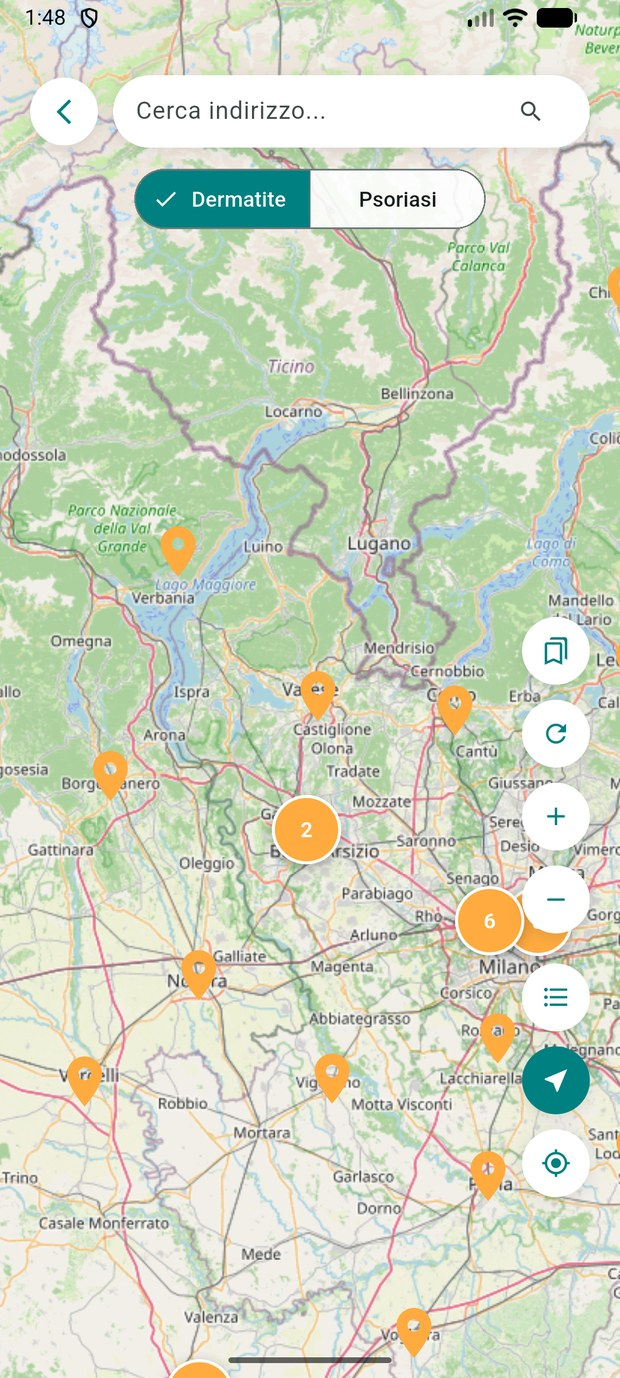
\includegraphics[width=\textwidth]{mappa-cluster}
  \caption{Cluster}
  \label{fig:sub-cluster}
\end{subfigure}\hfill
\begin{subfigure}[t]{0.3\textwidth}
  \centering
  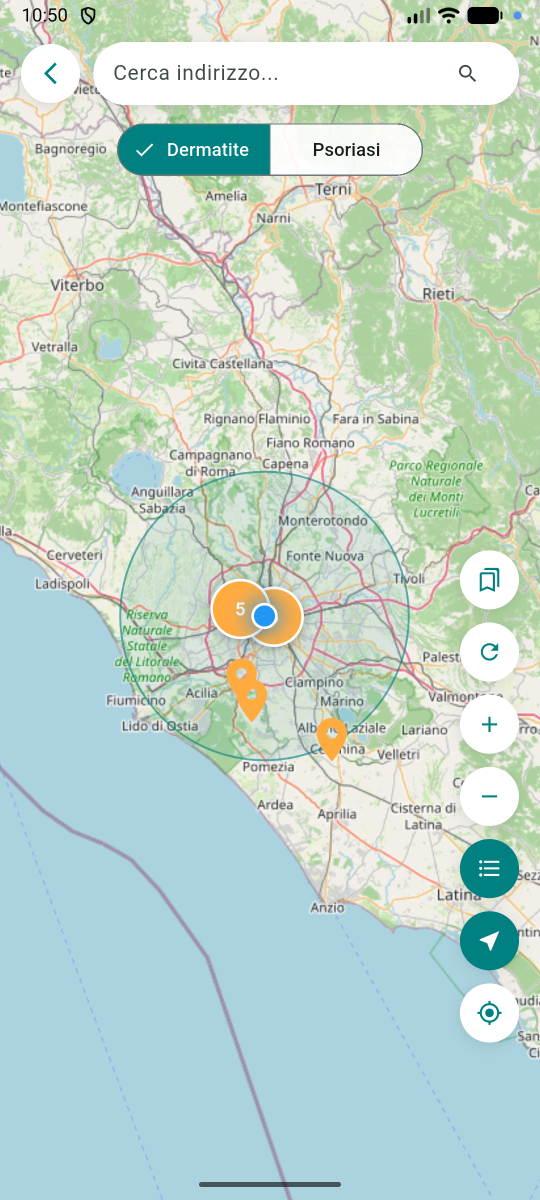
\includegraphics[width=\textwidth]{mappa-raggio-2}
  \caption{Filtro per raggio}
  \label{fig:sub-raggio}
\end{subfigure}\hfill
\begin{subfigure}[t]{0.3\textwidth}
  \centering
  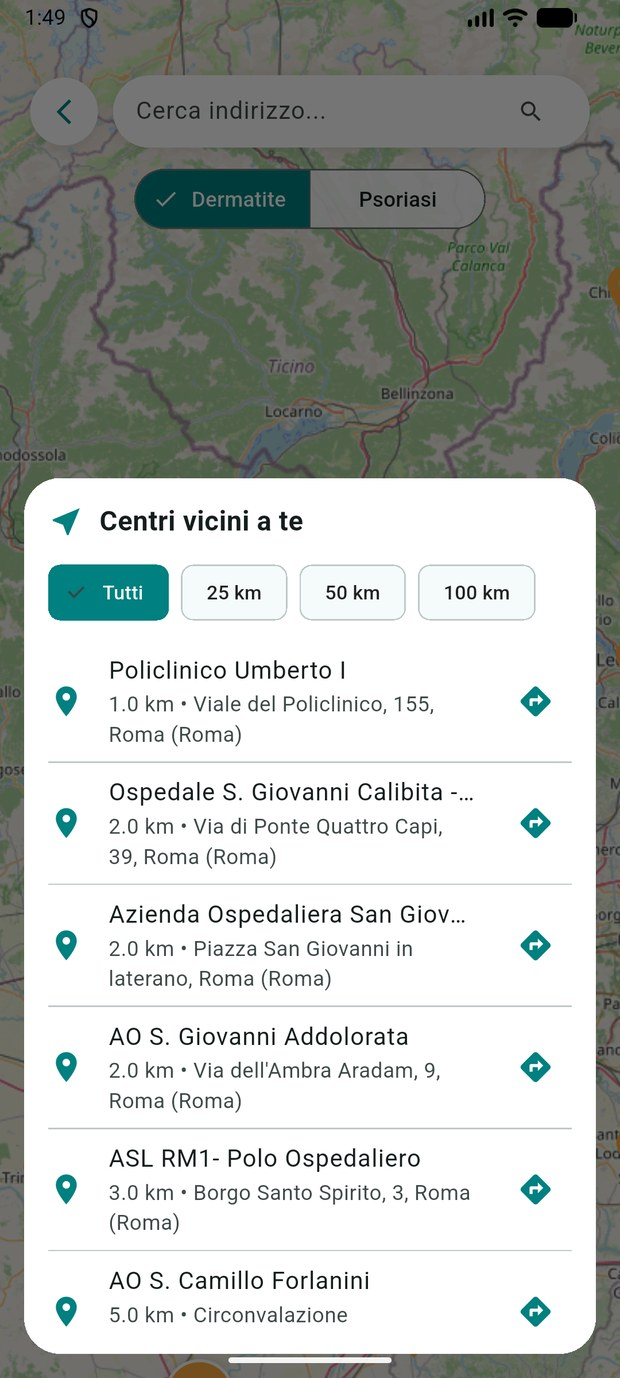
\includegraphics[width=\textwidth]{centri-vicini}
  \caption{Centri vicini}
  \label{fig:sub-vicini}
\end{subfigure}
\caption{Vista cartografica: cluster numerati, cerchio del filtro per raggio ed elenco ordinato per distanza.}
\label{fig:screen-mappa}
\end{figure}

%Nella figura \ref{fig:sub-cluster} si riconoscono le bolle numerate prodotte dall'algoritmo del paragrafo \ref{subsec:impl-clustering},
%con i marker singoli che convivono con i cluster nella stessa vista: sono le celle con un solo membro, disegnate come marker ordinari.
%Si nota anche la colonna dei comandi sul lato destro, nella metà inferiore dello schermo come richiede il requisito RNF-01.
%
%La figura \ref{fig:sub-raggio} mostra il cerchio del filtro attivo, con il riempimento tenue che delimita senza coprire
%il territorio sottostante.
%La figura \ref{fig:sub-vicini} riporta l'elenco per prossimità, con le scelte discrete del raggio in testa al pannello
%e la distanza formattata secondo gli scaglioni descritti al paragrafo \ref{subsec:impl-filtraggio}.

\begin{figure}[H]
\centering
\begin{subfigure}[t]{0.235\textwidth}
  \centering
  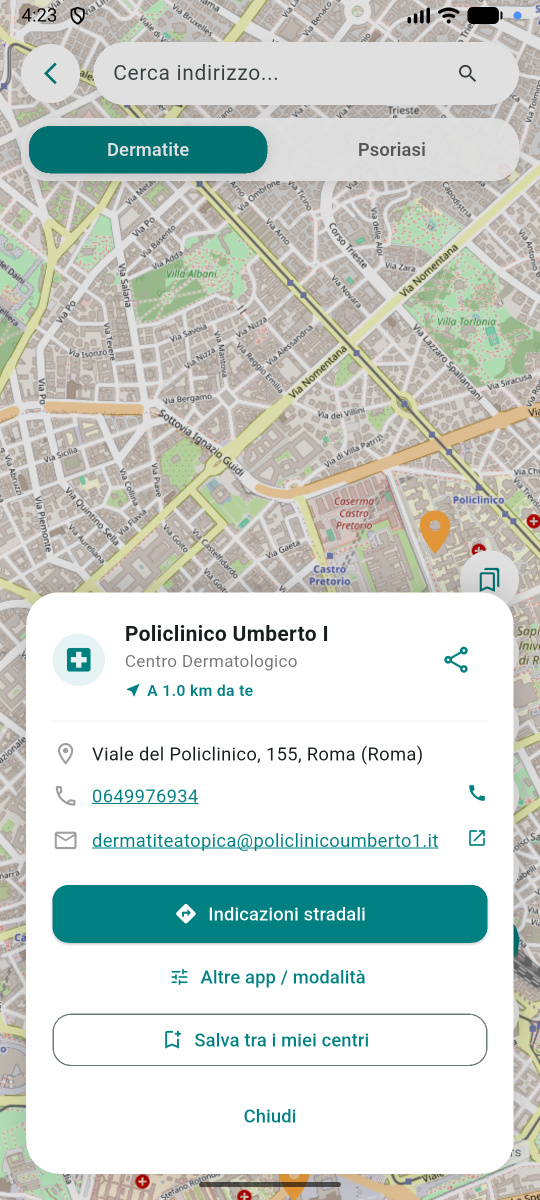
\includegraphics[width=\textwidth]{popup-centro}
  \caption{Scheda}
  \label{fig:sub-popup}
\end{subfigure}\hfill
\begin{subfigure}[t]{0.235\textwidth}
  \centering
  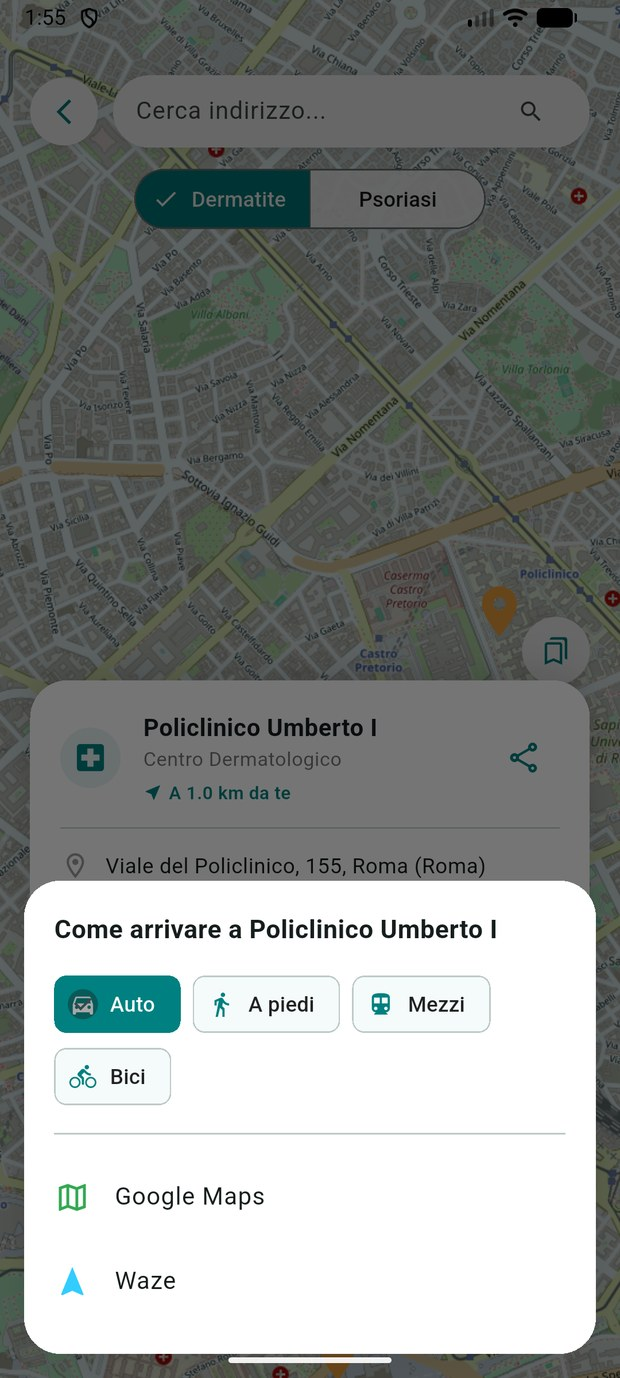
\includegraphics[width=\textwidth]{indicazioni}
  \caption{Percorso}
  \label{fig:sub-indicazioni}
\end{subfigure}\hfill
\begin{subfigure}[t]{0.235\textwidth}
  \centering
  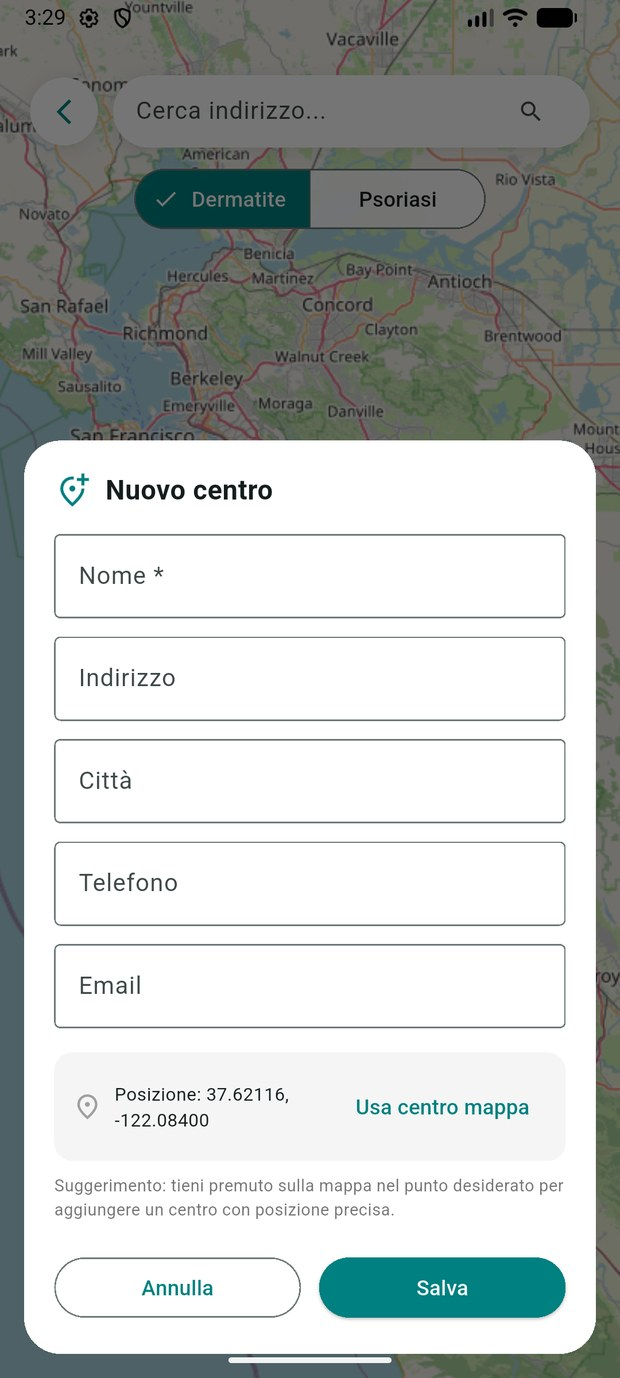
\includegraphics[width=\textwidth]{form-centro}
  \caption{Inserimento}
  \label{fig:sub-form}
\end{subfigure}\hfill
\begin{subfigure}[t]{0.235\textwidth}
  \centering
  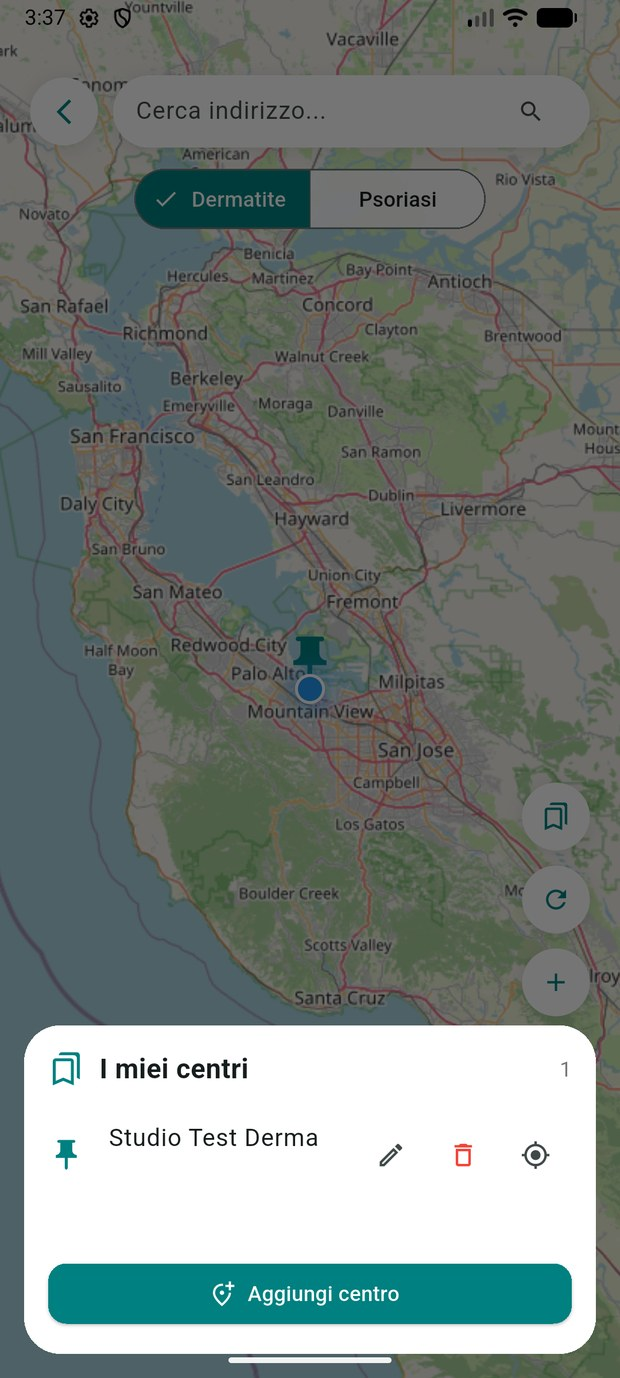
\includegraphics[width=\textwidth]{miei-centri}
  \caption{Centri propri}
  \label{fig:sub-miei}
\end{subfigure}
\caption{Pannelli modali: scheda della struttura, scelta del mezzo e dell'applicazione di navigazione, modulo di
inserimento ed elenco dei centri personalizzati.}
\label{fig:screen-schede}
\end{figure}

%I quattro pannelli della figura \ref{fig:screen-schede} rendono evidente la scelta discussa al paragrafo \ref{subsec:flusso-navigazione}:
%nessuno di essi occupa l'intero schermo, e la mappa resta visibile al di sopra, così che il contesto geografico non venga
%perso nel momento in cui si consultano i dettagli.
%Nella figura \ref{fig:sub-indicazioni} si vedono le scelte del mezzo di
%trasporto sopra l'elenco delle applicazioni di navigazione, disposizione che rispecchia l'ordine dei passi del caso d'uso UC-07,
%dove il mezzo viene scelto prima dell'applicazione.
%La figura \ref{fig:sub-form} mostra il modulo di inserimento con il riquadro
%della posizione acquisita dalla mappa e il comando di riallineamento descritto al paragrafo \ref{subsec:impl-validazione}.

\chapter{Testing}\label{ch:testing}

\section{Strategia di testing}\label{sec:strategia-testing}

%La verifica di un modulo come questo incontra una difficoltà di fondo: quasi tutto ciò che fa dipende da qualcosa che
%non controlla.
I dati arrivano da servizi terzi, la posizione arriva dal sistema operativo, le azioni finali vengono eseguite da
altre applicazioni, e la resa cartografica dipende da immagini scaricate dalla rete.
È opportuno sottoporre a test ciascuno di questi elementi.

La strategia adottata parte quindi da una domanda: che cosa sia verificabile in modo affidabile e ripetibile senza un
dispositivo collegato e senza dipendere dalla rete.
Sono quindi implementate due tipologie di verifica, riassunte nella tabella \ref{tab:strategia-test}.

\begin{table}[H]
\footnotesize
\begin{tabularx}{\textwidth}{@{}P{2.9cm} P{2.6cm} L@{}}
\toprule
\textbf{Livello} & \textbf{Strumento} & \textbf{Elemento verificato} \tabularnewline
\midrule
Unit Testing & Framework di test & Serializzazione dei centri personalizzati, lettura e scrittura
dell'archivio, calcolo delle distanze geodetiche \tabularnewline
% Test di widget & framework di test dell'interfaccia & Validazione del modulo di inserimento, comportamento in
% modifica, esito del salvataggio \tabularnewline
Test manuali & Dispositivo ed emulatore & Permessi di posizione, cluster, delega alle applicazioni esterne,
comportamento senza rete \tabularnewline
\bottomrule
\end{tabularx}
\caption{Verifiche effettuate e rispettivo elemento coinvolto.}
\label{tab:strategia-test}
\end{table}

%La maggior parte dei test sono anche i più veloci e i più vicini al codice \cite{sommervilleSoftwareEng, flutterTesting}.
Gli \textit{unit test} (test unitari) non richiedono alcun ambiente grafico e si eseguono in pochi secondi se non meno; i test manuali sono i più
lunghi e sono stati riservati a ciò che i primi non possono coprire.
% I test unitari non richiedono alcun ambiente grafico e si eseguono in una frazione di secondo; quelle di widget costruiscono
% un albero di componenti in memoria e simulano i tocchi, con un costo maggiore ma ancora senza dispositivo; i test manuali
% sono i più costosi e sono state riservate a ciò che le prime due non possono raggiungere.

% Occorre dire con precisione che cosa non è stato verificato in modo automatico: un elenco di test superati, senza il perimetro di
% ciò che copre, dice poco.
% Non esistono test sulle richieste di rete, che avrebbero richiesto un mock del client e la costruzione di risposte artificiali per
% ciascuna delle due sorgenti; non esistono test sulla macchina a stati dei permessi descritta al paragrafo \ref{sec:impl-localizzazione},
% che avrebbe richiesto la simulazione del canale di comunicazione con la piattaforma; non esistono test di integrazione che percorrano un
% caso d'uso completo su dispositivo, né test di prestazione strumentati.
% Le prime due assenze sono le più significative, perché riguardano proprio il codice più ricco di percorsi alternativi, ed è la sede in cui un
% lavoro di verifica più esteso dovrebbe cominciare.
%
% Un'ultima precisazione riguarda l'algoritmo di clustering del paragrafo \ref{subsec:impl-clustering}, che a rigore è la parte più facilmente
% verificabile di tutto il modulo, essendo una funzione che a partire da un elenco di coordinate e da un livello di zoom restituisce un
% elenco di cluster, senza dipendenze esterne.
% Test su quella funzione non sono stati scritti, perché il metodo che la realizza è privato della classe di stato del widget e non risulta
% raggiungibile dall'esterno; renderla verificabile avrebbe richiesto di estrarla in una unità autonoma, che è esattamente l'intervento che
% il requisito RNF-18 avrebbe dovuto imporre e che qui è stato disatteso.
% La correttezza dell'algoritmo è stata dunque valutata soltanto per osservazione diretta sulla mappa, e le proprietà numeriche riportate
% nella tabella \ref{tab:celle} sono verifiche analitiche, non risultati di test eseguiti.

\section{Unit test sulla logica applicativa}\label{sec:test-unitari}

La tabella \ref{tab:test-unitari} elenca gli Unit Test con esito e requisito a cui ciascuno si riferisce.

\begin{table}[H]
\footnotesize
\begin{tabularx}{\textwidth}{@{}P{0.6cm} L P{1.5cm}@{}}
\toprule
\textbf{N.} & \textbf{Caso di test} & \textbf{Esito} \tabularnewline
\midrule
\multicolumn{3}{@{}l}{\textbf{Serializzazione dei centri personalizzati} (RF-25)} \tabularnewline
1 & La conversione in JSON e il valore letto contengono tutti i campi & Superato \tabularnewline
2 & I campi vuoti opzionali o di soli spazi diventano \textit{null} & Superato \tabularnewline
3 & In assenza dell'elenco delle patologie vengono assegnate entrambe & Superato \tabularnewline
4 & Coordinate mancanti vengono azzerate senza sollevare errori & Superato \tabularnewline
5 & La copia con modifica altera solamente i campi richiesti e conserva l'identificatore & Superato \tabularnewline
\addlinespace
\multicolumn{3}{@{}l}{\textbf{Archiviazione locale dei centri personalizzati} (RF-25, RNF-08)} \tabularnewline
6 & Un archivio vuoto restituisce un elenco vuoto & Superato \tabularnewline
7 & Scrittura e successiva lettura mantengono i centri e nell'ordine corretto & Superato \tabularnewline
8 & Un contenuto corrotto non propaga l'errore e restituisce un elenco vuoto & Superato \tabularnewline
9 & Un documento JSON valido ma di forma diversa da un elenco viene ignorato & Superato \tabularnewline
\addlinespace
\multicolumn{3}{@{}l}{\textbf{Calcolo geodetico delle distanze} (RF-18, RF-19) } \tabularnewline
10 & La distanza Milano-Roma corrisponde al valore noto & Superato \tabularnewline
11 & La distanza di un punto da se stesso è nulla & Superato \tabularnewline
12 & La distanza è simmetrica rispetto agli estremi & Superato \tabularnewline
\bottomrule
\end{tabularx}
  \caption{Unit Test logica applicativa.}
\label{tab:test-unitari}
\end{table}

%I casi 2, 3 e 4 verificano comportamenti che l'uso normale non produce mai, ed è per questo che sono stati scritti.
%Un campo opzionale vuoto, un elenco di patologie assente e una coordinata mancante non si ottengono compilando il modulo
%di inserimento, che li rifiuterebbe; si ottengono leggendo un archivio scritto da una versione precedente dell'applicazione,
%oppure un archivio manomesso.
%Sono percorsi che senza un test automatico resterebbero non esercitati fino al momento in cui, sul dispositivo di un utente,
%provocherebbero un errore all'avvio.
%
%Lo stesso vale per i casi 8 e 9, che riguardano il requisito RNF-08.
%Il caso 8 inietta nell'archivio una stringa non interpretabile e verifica che la lettura restituisca un elenco vuoto invece di
%propagare l'errore.
%Il caso 9 è la variante meno evidente e più insidiosa: il contenuto è un documento JSON perfettamente valido, ma rappresenta un
%oggetto e non un elenco.
%Una lettura che si limitasse a intercettare gli errori di interpretazione supererebbe il caso 8 e fallirebbe il caso 9,
%perché l'interpretazione riuscirebbe e l'errore comparirebbe dopo, al primo tentativo di scorrere il risultato.
%La distinzione fra i due casi è il motivo per cui la lettura verifica esplicitamente il tipo del contenuto interpretato.
%
%Il caso 10 richiede una precisazione di metodo.
%Il valore atteso non è stato ricavato eseguendo il codice e registrandone il risultato, procedimento che avrebbe prodotto un
%test capace di rilevare soltanto le variazioni future ma non un errore già presente.
%È stato invece assunto dall'esterno il valore noto della distanza ortodromica fra le due città, circa quattrocentosettantasette
%chilometri, con una tolleranza di sei chilometri che assorbe le differenze fra i possibili raggi terrestri di riferimento e
%l'arbitrarietà delle coordinate scelte per rappresentare due città.
%Un test costruito in questo modo rileva anche l'errore che più facilmente si commette in questo ambito, cioè il calcolo di una
%distanza euclidea sui gradi: quel calcolo, sulle stesse coordinate, restituirebbe un valore incompatibile con la tolleranza, e
%il test fallirebbe.

% I casi 11 e 12 verificano due proprietà formali della funzione di distanza, cioè l'annullamento sull'argomento coincidente e la simmetria.
% Sono verifiche che sembrano superflue, poiché entrambe le proprietà sono garantite dalla formula impiegata, ma il loro costo è
% nullo e il loro valore è di sorveglianza: se in una versione futura la funzione di distanza venisse sostituita con una che tiene
% conto di un percorso stradale, la simmetria non sarebbe più garantita, e il test segnalerebbe il cambiamento di semantica invece
% di lasciarlo passare inosservato.

% I test di widget riguardano il modulo di inserimento dei centri personalizzati, e sono state scelte per due ragioni.
% La prima è che quel modulo contiene la logica di validazione descritta al paragrafo \ref{subsec:impl-validazione}, cioè la parte
% di interfaccia con il maggior numero di percorsi alternativi.
% La seconda è che si tratta di un componente che non dipende dalla rete, dalla posizione o dalla mappa, e che può quindi essere
% costruito in isolamento: ogni altra parte dell'interfaccia avrebbe richiesto un impianto di simulazione sproporzionato.
%
% Il modulo viene presentato nel test così come lo è in esercizio, cioè come pannello che sale dal basso aperto da una rotta, e non
% montato direttamente come componente isolato.
% La scelta è voluta: presentarlo nello stesso modo permette di intercettare il valore restituito alla chiusura, che è ciò che il
% codice chiamante riceve, e verifica quindi anche il fatto che il pannello si chiuda restituendo un centro valido, oppure che non si
% chiuda affatto quando la validazione non passa.
%
% La tabella \ref{tab:test-widget} elenca gli otto test con il rispettivo esito.
%
% \begin{table}[H]
% \footnotesize
% \begin{tabularx}{\textwidth}{@{}P{0.6cm} L P{2.1cm}@{}}
% \toprule
% \textbf{N.} & \textbf{Caso di test} & \textbf{Esito} \tabularnewline
% \midrule
% 1 & I campi obbligatori non compilati bloccano il salvataggio & non superato \tabularnewline
% 2 & In assenza sia di telefono sia di posta il salvataggio viene rifiutato & non superato \tabularnewline
% 3 & Un numero con troppe poche cifre viene segnalato & non superato \tabularnewline
% 4 & Un numero con prefisso non nazionale viene rifiutato & non superato \tabularnewline
% 5 & Un indirizzo di posta malformato viene segnalato & non superato \tabularnewline
% 6 & Un numero con prefisso internazionale viene accettato & non superato \tabularnewline
% 7 & Deselezionando ogni patologia il salvataggio è impedito & non superato \tabularnewline
% 8 & In modifica il modulo è precompilato e conserva l'identificatore & non superato \tabularnewline
% \bottomrule
% \end{tabularx}
% \caption{Test di widget sul modulo di inserimento: otto casi, nessuno superato per la ragione discussa nel testo.}
% \label{tab:test-widget}
% \end{table}
%
% Una colonna di esiti negativi richiede una spiegazione, e la spiegazione è la parte più istruttiva di questo capitolo.
% I test non falliscono perché le condizioni che verificano risultino disattese: tutte le condizioni sono soddisfatte, e in nessuno
% degli otto test si registra uno scostamento fra il valore atteso e quello osservato.
% I messaggi di errore compaiono dove devono comparire, il salvataggio viene impedito quando deve esserlo, il modulo in modifica risulta
% precompilato e conserva l'identificatore, e il numero con prefisso internazionale viene accettato producendo un centro valido.
% La logica di validazione, per quanto questi test la esercitano, è corretta.
%
% Il fallimento ha un'altra origine.
% Durante la costruzione dell'albero dei componenti l'applicazione stessa solleva un avviso del framework, ripetuto ventotto volte nel corso
% dell'esecuzione complessiva, e l'ambiente di test considera non superato ogni test nel corso del quale il framework segnali un'anomalia,
% indipendentemente dall'esito delle condizioni verificate.
% Gli otto test risultano quindi non superati a causa di un difetto del codice sottoposto a test, e non di un difetto dei test.
%
% Il difetto è questo.
% Le due righe con checkbox che permettono di scegliere le patologie sono componenti che disegnano il proprio sfondo e la propria animazione
% di tocco sulla superficie Material più vicina che le contiene.
% Nel modulo, però, fra quelle righe e la superficie Material fornita dal pannello si interpone il contenitore bianco con angoli arrotondati
% che dà al modulo il suo aspetto, e il pannello è dichiarato con fondo trasparente.
% La conseguenza è che l'animazione di tocco viene disegnata al di sotto del contenitore bianco, che la nasconde: premendo
% su una delle due righe l'utente non riceve alcun riscontro visivo dell'avvenuto tocco, mentre la selezione cambia effettivamente stato.
%
% Si tratta quindi della violazione di un requisito non funzionale, e precisamente del requisito RNF-03, che chiede un riscontro
% visivo immediato per ogni azione dell'utente.
% La gravità è contenuta, perché il checkbox cambia aspetto e l'esito dell'azione resta percepibile; l'elemento mancante è
% l'animazione che accompagna il tocco, cioè la conferma che il tocco è stato raccolto nel punto in cui è avvenuto.
% La correzione consiste nel racchiudere quelle righe in una propria superficie Material, oppure nell'ottenere il fondo bianco
% del modulo da un componente che sia esso stesso una superficie Material invece che da un contenitore decorato: in entrambi i
% casi si tratta della sostituzione di un componente.
%
% Il difetto non è stato corretto nella versione descritta, e lo riporto qui insieme al suo effetto sui test per una ragione di metodo.
% Nessuna delle verifiche manuali svolte durante lo sviluppo lo aveva rilevato, e non per distrazione: l'assenza di un'animazione di
% tocco su una riga che cambia comunque aspetto è precisamente il genere di difetto che l'occhio non nota, perché non c'è nulla di
% sbagliato da vedere ma soltanto qualcosa di corretto che manca.
% I test automatici lo hanno reso visibile al primo tentativo di esecuzione, prima ancora di essere state completate.
% è l'argomento più concreto a favore dei test automatici che questo lavoro ha prodotto, ed è anche per questo che ho preferito
% documentare la colonna di esiti negativi invece di sospendere la segnalazione nell'ambiente di test, che avrebbe restituito otto
% esiti positivi lasciando il difetto nel codice.

\section{Verifiche manuali}\label{sec:test-compatibilita}

Ciò che non è stato possibile verificare tramite i test automatici è stato collaudato manualmente su emulatore Android. %e su dispositivo Android fisico.
La tabella \ref{tab:test-manuali} riporta gli scenari testati con il proprio esito.

\begin{table}[H]
\footnotesize
\begin{tabularx}{\textwidth}{@{}P{4.0cm} L P{1.6cm}@{}}
\toprule
\textbf{Scenario} & \textbf{Comportamento atteso} & \textbf{Esito} \tabularnewline
\midrule
Permesso concesso & La mappa viene centrata sulla posizione e viene seguita dall'indicatore durante lo spostamento & Superato \tabularnewline
Permesso negato una volta & L'applicazione resta utilizzabile sulla schermata predefinita e la richiesta può essere ripresentata & Superato \tabularnewline
Permesso negato in modo permanente & Compare il collegamento alle impostazioni dell'applicazione & Superato \tabularnewline
Localizzazione disattivata & Compare il collegamento alle impostazioni di sistema, diverso dal precedente & Superato \tabularnewline
Avvio senza rete con cache presente & I marker compaiono dai dati conservati, senza avviso di errore & Superato \tabularnewline
Avvio senza rete e senza cache & Compare l'avviso di errore ed è disponibile il comando di aggiornamento & Superato \tabularnewline
Cluster in area urbana & I cluster riportano il numero corretto e si scompongono all'avvicinamento & Superato \tabularnewline
Spostamento continuo della viewport & I marker si aggiornano al termine del gesto e non durante & Superato \tabularnewline
Delega a navigatore, telefono e posta & Si apre l'applicazione selezionata con il dato precompilato & Superato \tabularnewline
Apertura della tastiera nella barra di ricerca & I comandi vengono nascosti e la mappa non si ridimensiona & Superato \tabularnewline
\bottomrule
\end{tabularx}
\caption{Scenari verificati manualmente su Android e relativo esito.}
\label{tab:test-manuali}
\end{table}

%L'ultima riga della tabella registra un difetto rilevato e corretto durante lo sviluppo, ed è il caso descritto al
%paragrafo \ref{subsec:design-mappa-centri}: all'apertura della tastiera i comandi flottanti risultavano parzialmente
%coperti dall'elenco dei suggerimenti.
%La correzione è quella descritta al paragrafo \ref{subsec:impl-ricerca}, cioè la ritrazione dei comandi durante la ricerca,
%valutata su tre indizi distinti invece che su uno solo.

%Sulla compatibilità fra le due piattaforme va dichiarata un limite.
%Non avendo a disposizione una macchina Apple, né un dispositivo iOS, la verifica su tale piattaforma non è stata svolta.
%Il codice è scritto per entrambe le piattaforme e i punti in cui le distingue sono espliciti, ma il comportamento su iOS
%resta previsto e non osservato.

%I punti che restano non verificati sono tre, e vale elencarli perché sono esattamente quelli in cui il codice contiene una
%diramazione dipendente dalla piattaforma.
%Il primo è la comparsa di Apple Maps fra le destinazioni di navigazione, subordinata al riconoscimento del sistema operativo.
%Il secondo è la ricaduta della modalità in bicicletta sul percorso automobilistico nel collegamento di Apple Maps, descritta
%nella tabella \ref{tab:navigazione}, che è stata ricavata dalla documentazione del collegamento e non da un test.
%Il terzo è la comparsa del testo di motivazione del permesso di posizione, dichiarato nel file di configurazione della piattaforma,
%di cui non è stato possibile osservare la resa effettiva nella finestra di sistema.

% Una nota infine sull'ambiente di esecuzione dei test di widget.
% Il modulo di inserimento è più alto di uno schermo di dimensioni predefinite, e i test impostano quindi esplicitamente una superficie
% di lavoro più estesa, ripristinandola al termine.
% Senza questo accorgimento i componenti collocati in fondo al modulo, fra cui il pulsante di conferma, non risulterebbero raggiungibili
% dai tocchi simulati, e i test fallirebbero per una ragione che non ha nulla a che vedere con il comportamento verificato.
% è un dettaglio tecnico, ma è anche un promemoria del fatto che un test di interfaccia verifica il componente dentro le condizioni che
% l'ambiente di test stabilisce, e che quelle condizioni vanno dichiarate insieme al risultato.

\chapter{Conclusioni}\label{ch:conclusioni}

\section{Risultati raggiunti}\label{sec:risultati-raggiunti}

Il lavoro ha prodotto una mappa funzionante, che raccoglie da elenchi pubblici i centri dermatologici dedicati
alla dermatite atopica e alla psoriasi, li mostra su una mappa interattiva con clustering dinamico dei marker, li filtra per
patologia e per distanza, %dalla posizione dell'utente,
li integra con voci inserite a mano e salvate sul dispositivo, e
delega ai programmi installati le azioni che seguono la consultazione come, per esempio, la creazione del percorso.

Rispetto alla domanda da cui il lavoro è partito, cioè dove si trovi il centro più vicino che segue una determinata patologia e
come raggiungerlo, la risposta è ora ottenibile con due tocchi a partire dall'apertura della schermata, rispetto alla ricerca manuale
degli elenchi o di diverse mappe online.
Il contributo non sta nei dati, che restano quelli censiti da altri, ma nel modo in cui vengono interrogati: per prossimità,
in un unico posto.
%invece che per appartenenza territoriale.

% Sul piano quantitativo la copertura della specifica è riassunta nella tabella \ref{tab:copertura} e distribuita graficamente nella
% figura \ref{fig:copertura}.
% La classificazione distingue i requisiti soddisfatti, quelli soddisfatti soltanto in parte e quelli non soddisfatti, e in
% questa sede la colonna che conta è la terza: un riepilogo che dichiarasse tutto soddisfatto sarebbe più gradevole e meno utile.
%
% \begin{figure}[H]
% \centering
% \begin{tikzpicture}
% \begin{axis}[
%   ybar, bar width=1.1cm,
%   width=\textwidth - 2.6cm, height=6.4cm,
%   ymin=0, ymax=52,
%   ytick distance=10,
%   ylabel={Requisiti},
%   symbolic x coords={Soddisfatti, Parziali, Non soddisfatti},
%   xtick=data,
%   x tick label style={font=\footnotesize, yshift=-2pt},
%   y tick label style={font=\footnotesize},
%   tick align=outside,
%   axis lines=left,
%   nodes near coords,
%   nodes near coords style={font=\footnotesize},
%   enlarge x limits=0.3
% ]
% \addplot[fill=black!25, draw=black!55] coordinates {(Soddisfatti,43) (Parziali,11) (Non soddisfatti,2)};
% \end{axis}
% \end{tikzpicture}
% \caption{Distribuzione della copertura della specifica: quarantatrè requisiti soddisfatti, undici soddisfatti soltanto
% in parte e due non soddisfatti.}
% \label{fig:copertura}
% \end{figure}
%
% \begin{table}[H]
% \centering
% \footnotesize
% \begin{tabular}{@{}l c c c c@{}}
% \toprule
% \textbf{Categoria} & \textbf{Totale} & \textbf{Soddisfatti} & \textbf{Parziali} & \textbf{Non soddisfatti} \tabularnewline
% \midrule
% Requisiti funzionali & 38 & 33 & 4 & 1 \tabularnewline
% Requisiti non funzionali & 18 & 10 & 7 & 1 \tabularnewline
% \midrule
% \textbf{Totale} & \textbf{56} & \textbf{43} & \textbf{11} & \textbf{2} \tabularnewline
% \bottomrule
% \end{tabular}
% \caption{Copertura della specifica nella versione realizzata.}
% \label{tab:copertura}
% \end{table}
%
% La tabella \ref{tab:scostamenti} elenca uno per uno gli scostamenti, con la natura di ciascuno.
% è la parte del riepilogo che ha richiesto più lavoro, perché diversi di questi scostamenti non erano noti durante lo sviluppo
% e sono emersi dal riesame sistematico del codice svolto per la scrittura dei capitoli precedenti: scrivere che cosa fa un
% programma è un modo efficace di accorgersi di che cosa non fa.
%
% \begin{table}[H]
% \footnotesize
% \begin{tabularx}{\textwidth}{@{}P{2.0cm} P{1.9cm} L@{}}
% \toprule
% \textbf{Requisito} & \textbf{Stato} & \textbf{Scostamento rilevato} \tabularnewline
% \midrule
% RF-07 & non soddisfatto & L'attribuzione della sorgente cartografica non è presente sulla mappa \tabularnewline
% RNF-12 & non soddisfatto & Conseguenza del precedente: obbligo di licenza non rispettato \tabularnewline
% \addlinespace
% RF-02 & parziale & La ricaduta sulla sorgente alternativa avviene senza avvisare che i centri mostrati non sono specifici
% della patologia richiesta \tabularnewline
% RF-23 & parziale & Il filtro per raggio esclude i centri personalizzati dall'elenco ma non dalla mappa \tabularnewline
% RF-29 & parziale & I centri personalizzati sono distinguibili nell'elenco ma non sulla mappa, dove usano lo stesso marker
% dei centri remoti \tabularnewline
% RF-34 & parziale & Un numero contenente un trattino viene troncato nella composizione della chiamata \tabularnewline
% \addlinespace
% RNF-02 & parziale & I comandi circolari flottanti misurano 45 punti di lato, contro i 48 richiesti \tabularnewline
% RNF-03 & parziale & Le righe di selezione della patologia non mostrano l'animazione di tocco \tabularnewline
% RNF-04 & parziale & Il messaggio di errore della ricerca riporta il testo tecnico dell'eccezione \tabularnewline
% RNF-08 & parziale & Le due richieste alla geocodifica non hanno limite di attesa, che è presente solo sugli elenchi \tabularnewline
% RNF-13 & parziale & L'identificativo trasmesso con le richieste dei tile è quello di esempio; il rinvio sulla digitazione
% riduce le richieste alla geocodifica senza garantirne formalmente la frequenza \tabularnewline
% RNF-17 & parziale & L'indipendenza dallo schema remoto è ottenuta nel comportamento ma non nella struttura, per la dispersione
% delle catene di alias \tabularnewline
% RNF-18 & parziale & La logica di clustering non è raggiungibile da un test automatico \tabularnewline
% \bottomrule
% \end{tabularx}
% \caption{Scostamenti rilevati rispetto alla specifica, con la relativa natura.}
% \label{tab:scostamenti}
% \end{table}

Fra i risultati va contato anche il sistema di verifica, con dodici unit test superati sulla serializzazione,
persistenza e sul calcolo geodetico.
% , e otto test di widget sulla validazione del modulo di inserimento.
% Queste ultime, come descritto al paragrafo \ref{sec:test-ui}, risultano tutte non superate, e non perché le condizioni
% verificate siano disattese, ma perché hanno reso visibile un difetto dell'interfaccia che nessun test manuale aveva rilevato.
% è l'esito che considero più significativo dell'intera attività di verifica, e non a dispetto della colonna di esiti negativi
% ma proprio in virtù di essa.

A livello personale, il lavoro ha avuto un valore che merita di essere menzionato.
%Sul piano personale il lavoro ha avuto un esito che vale registrare.
La scelta iniziale di rinunciare a una piattaforma di mappe commerciale, motivata al paragrafo \ref{subsec:scelta-flutter} da
ragioni di costo e di riproducibilità, ha comportato la necessità di costruire a mano funzioni che quella piattaforma avrebbe fornito
comprese nel prezzo.
Di conseguenza, il modulo dell'algoritmo di clustering del paragrafo \ref{subsec:impl-clustering}
e i ragionamenti annessi esistono perché quella funzione non era disponibile.
% Che la costante di quell'algoritmo sia stata trovata per tentativi e ne abbia compreso il significato geometrico soltanto
% in un secondo momento, ricostruendolo per scrivere queste pagine, è a sua volta un risultato del lavoro di stesura.

\section{Criticità e limiti attuali}\label{sec:limiti-attuali}

I limiti che restano sono riconducibili a due punti.
\begin{enumerate}
    \item La cache degli elenchi non ha una scadenza, per cui i dati mostrati restano quelli dell'ultimo \textit{download} finché l'utente
    non richiede esplicitamente un aggiornamento, come discusso al paragrafo \ref{subsec:strategia-cache}.
    \item Il modulo dipende dagli elenchi pubblici di terzi, sui quali non si ha controllo né sul formato né sulla loro disponibilità.
    Le opzioni migliori valutate per rimuovere questi limiti sono tema del paragrafo \ref{sec:sviluppi-futuri}.
\end{enumerate}

% I limiti si dividono in tre famiglie, che hanno natura ed esigibilità diverse: le omissioni da correggere, i compromessi di
% progettazione consapevoli, e i vincoli imposti dalle condizioni in cui il lavoro si è svolto.
%
% La prima famiglia comprende gli scostamenti della tabella \ref{tab:scostamenti} e va corretta senza discussione.
% Il primo per importanza è l'assenza dell'attribuzione cartografica: non è un difetto di comodità ma il mancato rispetto di un
% obbligo di licenza \cite{osmCopyright}, e la sua correzione richiede l'aggiunta di un singolo componente fra i livelli della mappa.
% Sono dello stesso genere l'identificativo di esempio trasmesso con le richieste dei tile, la mancanza del limite di attesa sulle
% richieste alla geocodifica, il messaggio di errore che riporta il testo dell'eccezione, il troncamento dei numeri contenenti
% un trattino e la dimensione dei comandi circolari, che va portata da quarantacinque a quarantotto punti.
% Nessuno di questi interventi è oneroso e ciascuno è localizzato.
%
% Restano i due difetti che rendono i centri personalizzati meno distinguibili e meno coerenti di quanto la specifica preveda.
% Sulla mappa usano lo stesso marker dei centri remoti, quando dovrebbero essere riconoscibili a vista, motivo per cui il requisito
% RF-29 risulta soddisfatto solo in parte; il filtro per raggio, inoltre, li esclude dall'elenco ma non dalla mappa, producendo la
% situazione poco difendibile di un centro che non compare fra i risultati mentre il suo marker resta visibile.
% Entrambi derivano dalla stessa scelta implementativa, cioè il livello separato e non sottoposto alla selezione descritto al
% paragrafo \ref{subsec:impl-marker}, e si correggerebbero facendo attraversare a quei centri lo stesso percorso dei centri remoti.
%
% La seconda famiglia comprende i compromessi assunti in modo consapevole, che non sono difetti ma scelte con un costo.
% Il più rilevante è la politica della cache descritta al paragrafo \ref{subsec:strategia-cache}: in assenza di una scadenza,
% un elenco già presente in memoria non viene mai riscaricato spontaneamente, e l'utente può consultare dati vecchi senza che
% nulla lo segnali.
% La correzione naturale è l'associazione di un istante di scaricamento a ciascun elenco conservato, con un aggiornamento
% automatico oltre una certa età e un'indicazione della data del dato mostrato.
%
% Allo stesso gruppo appartiene la dispersione delle catene di alias discussa al paragrafo \ref{subsec:modello-centri}, che rende
% l'aggiunta di una terza sorgente più costosa di quanto dovrebbe, e la ricaduta silenziosa fra le due sorgenti descritta al
% paragrafo \ref{subsec:impl-endpoint}, che mostra centri non specifici della patologia richiesta senza dichiararlo.
% Vi appartiene infine la natura geodetica di tutte le distanze mostrate: sono misurate in linea d'aria, e in territorio montano
% lo scostamento dal percorso reale può essere considerevole.
%
% La terza famiglia raccoglie i limiti imposti dalle condizioni del lavoro, e il principale è l'assenza di qualunque verifica su
% iOS, dichiarata al paragrafo \ref{sec:test-compatibilita}.
% Il codice è scritto per entrambe le piattaforme e i tre punti in cui le distingue sono espliciti, ma nessuno di essi è stato
% osservato in esecuzione; finché quella verifica non avviene, il supporto a iOS resta una previsione.
% Allo stesso ordine appartiene l'impossibilità di sottoporre a test automatico l'algoritmo di clustering, che non dipende da
% un vincolo esterno ma da una scelta di collocazione del codice, e che il requisito RNF-18 avrebbe dovuto prevenire.
%
% Resta da ricordare il limite che discende dalla premessa architetturale, cioè l'assenza di un servizio proprio.
% Il modulo dipende per i dati da due elenchi pubblicati da terzi, sui quali non ha alcun controllo e nessun preavviso di modifica:
% un cambiamento di formato deciso alla sorgente lo rende inutilizzabile fino a un aggiornamento dell'applicazione, e la chiusura
% di una delle due sorgenti ne dimezza il contenuto.
% La resistenza costruita nel livello di acquisizione, con la ricaduta fra sorgenti e la conservazione locale, attenua il problema
% ma non lo elimina, perché sposta soltanto in avanti il momento in cui l'assenza del dato diventa visibile.

\section{Sviluppi futuri}\label{sec:sviluppi-futuri}

Le opzioni di sviluppo future che sembrano più opportune non sono l'aggiunta di nuove funzioni, %di cui il modulo non ha particolare bisogno,
ma la rimozione dei limiti individuati nel paragrafo precedente.
Le tre che seguono sono ordinate per rapporto di beneficio/costo.%, e la prima è anche quella dall'effetto più ampio.

\subsection{Un livello intermedio di normalizzazione}\label{subsec:futuro-backend}

L'intervento con l'effetto più ampio consiste nell'integrare fra le sorgenti pubbliche e l'applicazione un servizio
proprio (come un \textit{middleware} o un'\textit{API}), che interroghi periodicamente gli elenchi originali, ne normalizzi
il contenuto una volta ed esponga al client un unico formato stabile.
%Questo è un elemento che non è stato ancora sviluppato, per le ragioni mostrate al
%paragrafo \ref{sec:architettura-sistema}.
% , e il riesame conclusivo mostra quanto quella rinuncia sia costata.

Un servizio di questo genere risolverebbe tre limiti distinti:

\begin{enumerate}
    \item Renderebbe superflue le catene di alias nel codice, perché l'applicazione riceverebbe record già omogenei e
    i nomi dei campi resterebbero confinati nel servizio.
    \item Sul lato del servizio permetterebbe di riconoscere i cambiamenti di formato delle sorgenti, che oggi si manifestano soltanto
    sul dispositivo dell'utente e sotto forma di elenco vuoto o malformato.
    \item Ridurrebbe drasticamente le richieste dirette ai servizi pubblici, in quanto le interrogazioni verrebbero effettuate da
    un solo ente a intervalli regolari invece che da ciascuna copia dell'applicazione.
\end{enumerate}



% , allineando il comportamento alle politiche d'uso
% che al paragrafo \ref{sec:limiti-attuali} risultano rispettate solo in parte

%L'altra faccia è il costo: un servizio va ospitato, mantenuto, sorvegliato e finanziato, e introduce un punto di guasto
%che oggi non esiste.
%È per questo che la scelta iniziale resta difendibile nel contesto di una tesi. Il modulo attuale, con tutti i suoi limiti,
%funziona senza che nessuno se ne prenda cura.

\subsection{Sincronizzazione fra dispositivi}\label{subsec:futuro-cloud}

I centri inseriti dall'utente vivono ad oggi soltanto sul dispositivo su cui sono stati creati.
Cambiando telefono vengono persi, e non esiste modo di consultarli da un secondo dispositivo.
Una sincronizzazione remota risolverebbe entrambi i problemi, e a livello tecnico sarebbe integrabile con la base di dati
già esistente.
Di fatto i centri personalizzati hanno già una rappresentazione tipizzata, una serializzazione simmetrica
e un identificatore stabile, ossia i tre requisiti principali di un tale sistema.

Rimarrebbe comunque un aspetto delicato: non tanto la sincronizzazione in sé, quanto ciò che essa comporta sul piano della riservatezza.
L'applicazione, nella versione attuale, non richiede alcuna registrazione e non trasmette all'esterno alcun dato personale,
come stabiliscono i requisiti RNF-10 e RNF-11; l'elenco dei centri dermatologici che una persona salva è un'informazione
da cui si potrebbe presumere la sua condizione di salute, e trasferirla su un servizio remoto la trasforma in un dato
sanitario personale custodito da terzi, con le conseguenze normative che ne derivano.
Una sincronizzazione realizzata senza affrontare questo punto peggiorerebbe l'applicazione invece di migliorarla, e la direzione
corretta sarebbe una cifratura eseguita sul dispositivo con una chiave che il servizio non possiede, in modo che il servizio
conservi dati che non è in grado di leggere nemmeno in caso esso venisse violato.
Si tratterebbe di crittografia \textit{end-to-end} basata su protocolli e standard moderni. %e rischi in caso di perdita delle chiavi.
%Un ulteriore possibile miglioramento, di natura diversa, consisterebbe nel permettere all'utente di proporre alle sorgenti originali le
%strutture che ha salvato e che negli elenchi pubblici non compaiono.
%Chiuderebbe il ciclo fra i due ruoli: chi consuma l'elenco è anche nella posizione migliore per accorgersi di ciò che
%manca, e restituirebbe valore ai portali da cui il progetto prende i propri dati; richiederebbe però una moderazione redazionale,
%che è un problema più organizzativo piuttosto che informatico.

\subsection{Percorsi}\label{subsec:futuro-percorsi}

Tutte le distanze mostrate dal modulo sono geodetiche (sono corrette in base alla curvatura terrestre), limitazione
discussa al paragrafo \ref{subsec:impl-filtraggio}.
L'introduzione di un servizio di \textit{routing} permetterebbe di ordinare i centri per il tempo di viaggio effettivo
invece che per distanza in linea d'aria, grandezza a cui l'utente è realmente interessato.
%Per esempio, in un contesto montano, o in un'area urbana congestionata, il centro geograficamente più vicino non è necessariamente
%quello alla distanza minore in linea d'aria o con la strada più corta (a causa di fattori come il traffico).
%Il cambiamento trasformerebbe l'ordinamento dell'elenco dei centri più vicini. ed è anche
%il motivo per cui uno degli unit test del paragrafo \ref{sec:test-unitari} verifica la simmetria della distanza: un instradamento
%su rete stradale non è simmetrico, e quel test segnalerebbe il cambiamento invece di ignorarlo.

%Lato grafico, il passaggio dai tile raster ad una mappa vettoriale porterebbe due vantaggi:
%
%\begin{enumerate}
%    \item La nitidezza a qualunque livello di ingrandimento e su qualunque densità di schermo (\textit{DPI}), che le immagini raster non possono garantire.
%    \item La possibilità di personalizzare lo stile della mappa attenuando gli elementi meno importanti.
%    Per esempio, una mappa in cui le strutture sanitarie vengano evidenziate e il resto del contesto
%    sia reso più tenue metterebbe in risalto l'informazione che l'utente sta cercando.
%\end{enumerate}
%
%
%
%Un'ultima funzione utile sarebbe il \textit{predownload} in locale dei tile di un'area scelta dall'utente, per
%consultare la mappa in assenza di rete.
%Attualmente il salvataggio in locale riguarda soltanto gli elenchi dei centri, come descritto al paragrafo \ref{subsec:strategia-cache}, e
%in assenza di rete i marker compaiono su uno sfondo vuoto.
%Quindi i marker restano disponibili, ma il contesto geografico che li rende leggibili viene perso.
%Su questa strada occorrerebbe procedere con criterio per rispettare la politica d'uso (\textit{ToS}) dei tile pubblici, che vieta espressamente
%il \textit{download} massivo di aree \cite{osmTilePolicy}, e che renderebbe quindi necessario l'utilizzo di un provider diverso oppure
%la predisposizione di un proprio servizio di tile.


% ----------------------
% ---- BIBLIOGRAPHY ----
% ----------------------
\backmatter
\sloppy % serve a non far andare i link oltre ai margini
\printbibliography[nottype=online, heading=bibintoc, title=Bibliografia]
\printbibliography[type=online, heading=bibintoc, title=Sitografia]

% ----------------------
% ---- DOCUMENT END ----
% ----------------------
\end{document}
